% reducesymm/blog/2modesBB.tex
% $Author$ $Date$

% Predrag 2013-08-10 Burak, git version only

\noindent
{\color{red} Do edit this git file (created 2013-08-10),
it is a new addition to the original svn version (which for now
stays untouched, the mother version is still the svn one).
}
\bigskip\bigskip

\subsection{{\twoMode} writeup}
\label{chap:2modesBBproj}

\begin{description}

\item[2013-07-25  Predrag] This is \BBedit{an example of Burak's edit},
and here is an internal footnote\BB{An internal footnote by Burak.}. They
are useful when you change something n the middle of a text, rather then
just append the newest blog post. Please remove the color from my
\PCedit{edits} as you read them and approve them, and I'll do the same
for yours.

% \item[2013-08-13  Predrag to Burak] Please define \eqv, \reqv, \po,
% and \rpo\ here, in form suitable for pasting into the putative
% \twoMode\ slicing paper.

    \PCedit{
\item[2013-08-14  Predrag]
Your definition of a \reqv\ is correct for one-parameter $\Group$, but we
will have to rethink it for $N$\dmn\ Lie group $\Group$. In that case the
time trajectory is a 1\dmn\ curve, generically tracing out the $N$\dmn\
group orbit quasiperiodically. Probably a
\HREF{http://www.streamsound.dk/book1/chaos/chaos.html\#205/z} {better
definition} (click on magenta hyperlinks!) would be that
$\vel({\ssp_{\ssp}}) \in \pS_{EQ}$, and than show that this is then true
true anywhere on the group orbit. Perhaps using
\HREF{http://www.streamsound.dk/book1/chaos/chaos.html\#204/z} {Lie
derivatives}...
    }

\end{description}

% [2013-08-13 Burak]
\noindent{\bf Invariant solutions:}                     \toCB
A point $\ssp_{EQ}$ is an \eqv\ if the velocity function evaluated at this
point is 0, namely, $\dot{\ssp}|_{\ssp=\ssp_{EQ}} = \vel({\ssp_{EQ}}) = 0$.
Orbit of
a point $\ssp$ of a $\Group$-equivariant flow is called a \reqv\ if for any
time evolved point on the orbit $\ssp(\tau) = f^{\tau}(\ssp_{REQ})$ there
exists a parameter $\phi$ such that $\ssp(\tau) = \Group(\phi) \ssp$, in other
words, a time orbit is a \reqv\ if it coincides with the group orbit.
 A
point $\ssp$ is on a \po\ if its trajectory passes through itself after some
certain time \period{}, namely $\ssp = f^{\period{}}(\ssp)$. Finally, a point $\ssp$ of a
$\Group$-equivariant flow is said to be on a \rpo\ if there exists a
point $\ssp(\period{}) = f^\period{}(\ssp)$ on the orbit of $\ssp$, such that it satisfies $\ssp(\period{}) =
\LieEl(\phi) \ssp$ for a certain $\phi$.

\textbf{[2013-09-30  Predrag]}
Experimenting with how to compare parameter sets, starting with the set
\refeq{eq:PKparamsfinal}
\bea
\mu_1&=&-2.8023, \mu_2=1, a_1=-1, a_2=-2.6636
    \continue
b_1  &=& 0, b_2=0, c_1=-4.1122, c_2=1.8854, e_2=1
\,.
\label{eq:PKparamsfinal1}
\eea

\begin{tabular}{l|l|l|}
  & \refeq{eq:PKparamsfinal} & . \\
  \hline
  % after \\: \hline or \cline{col1-col2} \cline{col3-col4} ...
  $\mu_1$ & -2.8023 & . \\
  $\mu_2$ & 1       & . \\
  $e_1$   & 0       & 0 \\
  $e_2$   & 1       & . \\
  $a_1$   & -1      & . \\
  $a_2$   & -2.6636 & . \\
  $b_1$   & 0       & . \\
  $b_2$   & 0       & . \\
  $c_1$   & -4.1122 & . \\
  $c_2$   & 1.8854  & . \\
  $\#_{eqv}$ & . & . \\
  \hline
\end{tabular}



\subsection{Burak's {\twoMode} blog}
\label{chap:2modesBBblog}

\begin{description}
\item[2012-05-07  Predrag to Chaos Gang] It's not over until it is over.

\item[2013-07-25  Predrag]
 - instead of computing \cLf\ one more
time, how about giving a try to \twoMode\ $\SOn{2}$-equivariant flow,
defined in
\\
\texttt{reducesymm/cgang/2modes.tex}
\\ (you can get it by a click
\HREF{../cgang/2modes.pdf}{here}, provided you had already pdflatex-ed
2modes.tex). Have a look at it, and then meet with Daniel Borrero, 3. floor
Schatz lab, who can walk you through what we had already done and learned
(all in the 2modes.pdf blog). You can play with it for -let's say- two
weeks, see whether you can find an interesting strange attractor worth
slicing. If that does not work out, we'll give up, and go to \KS\ instead,
which is much more important for our overall goals...

\item[2013-08-06 Predrag]
A more precise statement of what we are trying to achieve with this model is
in \emph{reducesymm/cgang/2modes.tex:}

``For the 4\dmn\ model at hand are using the invariant polynomials
$\{u,v,w,q\}$ dynamics only to develop intuition, but to illustrate the
general \mslices, everything has to do be done in $\pS =
\{x_1,x_2,y_1,y_2\}$ and \slice\ $\pSRed$ as well. You can see that even
for the simplest conceivable $\SOn{2}$ 4-dimensional flow one has to
think about how to construct the invariant polynomials basis, and it is
hard to imagine how anyone could do that for very high\dmn\ flows.''

If we can find a nice strange attractor with comparable amplitudes in the
two modes, and show how to slice it, that would be the simplest example of
power of slicing, as the symmetry-reduced dynamics is 3\dmn\ and something
a human can look at, turn around as 3\dmn\ Mathematica or Matlab figure.

If in addition it turns out that my favorite Sobolev norm (read
\texttt{reducesymm/blog/norms.tex}) reduces the number of local slice
hyperplanes needed to cover the attractor, I'll be doubly happy.

\begin{figure}[ht]
\begin{center}
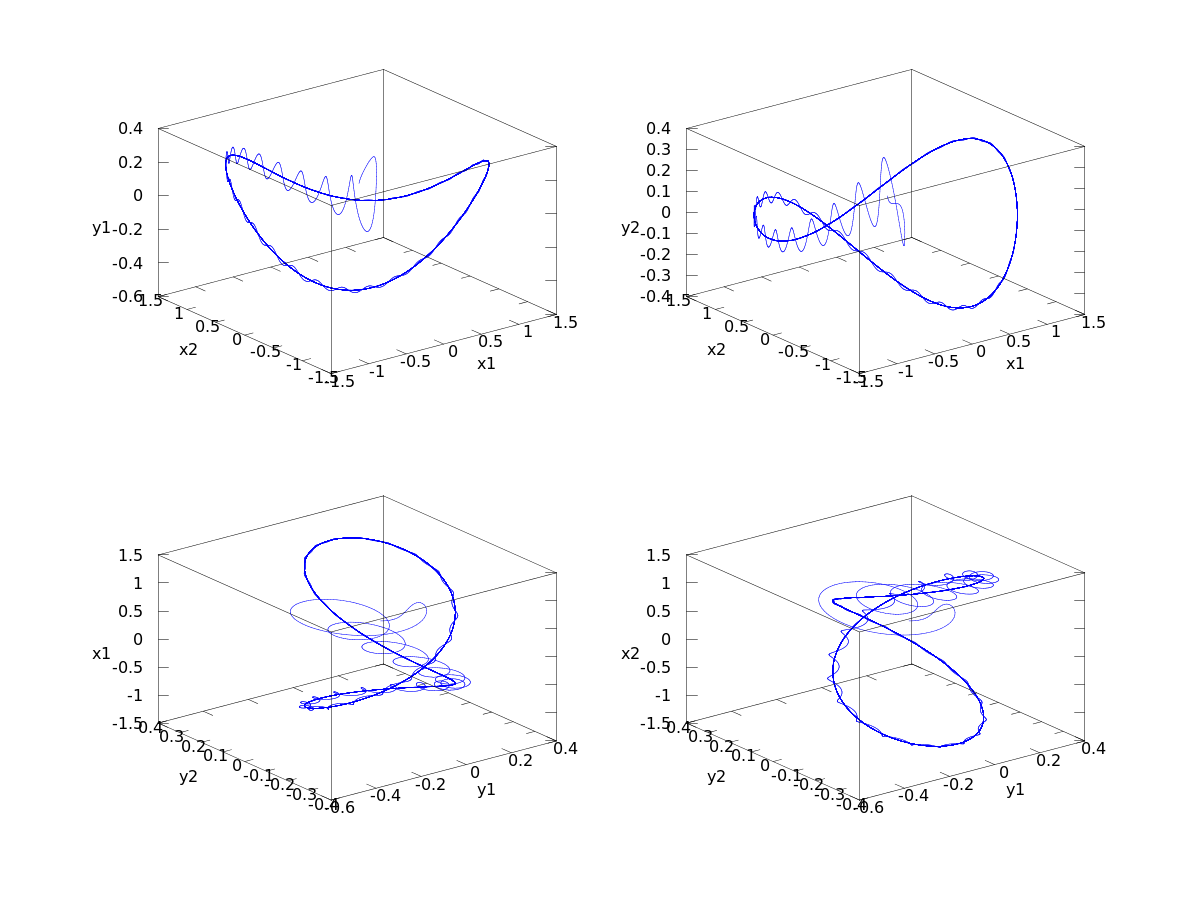
\includegraphics[width=0.9\textwidth]{PKperorb}
\end{center}
\caption{A typical
%Predrag 2013-08-05 removed ``periodic orbit''
attractive \reqv\  of \twoMode\ flow.}
\label{fig:PKperorb}
\end{figure}

\item[2013-08-05  Burak] I read the \twoMode\ blog and
    \HREF{http://chaosbook.org/paper.shtml\#stability} {Chapter 4} -
    {\em Local stability}, confirmed most of the findings in blog,
    naively experimented on the parameters of the system in $x_i, y_i$
    basis tried to find equilibria, got nothing, then talked to Daniel,
    and re-read the blog and come up with a Monte-Carlo (kind of)
    algorithm hoping that it could get me a strange attractor. So far,
    I only got periodic orbits. \refFig{fig:PKperorb} is a typical one.

\item[2013-08-06 Predrag]
Got worried that there were no updates for 11 days - how about if agree
on a schedule, let's say git pushes
\textcolor[rgb]{1.00,0.00,0.00}{every Monday and Friday}?

                                            \toCB
The \po s (actually, \reqva) that you find are presumably \emph{limit
cycles}. In ChaosBook I define `limit cycles' as \po s which are strictly
exponentially attracting forward in time. Parenthetically, in her thesis
De Witte\rf{DWRGK13,DeWitte13} defines a `limit cycle' as an ``isolated
periodic orbit'' thusly:

``A cycle of a continuous-time dynamical system, in a neighbourhood of
which there are no other cycles, is called a limit cycle.''

That presumably has advantage of being true for both directions of time,
but I do not think we need to get that finicky...


\item[2013-08-05  Burak]
    Here is what I did:
\begin{itemize}
\item
Generate pseudo-random set of parameters ensuring $\mu_1 > -\mu_2 > 0$, $c_1 = 1$ and $c_2 = -1$ as suggested in [2012-04-29 Predrag] and [2012-08-06 Edgar Knobloch]
\item
Numerically compute roots of \refeq{PKinvEqs5a} in $u>0, v>0$ region
starting from pseudo-random pair of points $(u,v)$, to find an
equilibrium in invariant polynomial basis.
\bea
\tilde{f}(\tilde{u},\tilde{v}) &=&
  \tilde{u}\,A_1 - \tilde{v}\,A_2 = 0 %Double checked DB 04-30-2012
\,,\qquad\qquad\qquad\qquad  deg(f) = 2
\continue
\tilde{g}(\tilde{u},\tilde{v}) &=&  %Double checked DB 04-30-2012
 \left(A_1^2
 - c_1\,\tilde{v}\right)
 \left(\tilde{u}+2\,\tilde{v}\right)^2
 +e_2^2\,\tilde{v}^2 = 0
\,,\qquad  deg(g) = 4
\continue
&& \mbox{where }
A_1 = \mu_1+\tilde{a_1}\,\tilde{u}+\tilde{b_1}\,\tilde{v},
\continue
&& \,\,\,\,\qquad A_2 = \mu_2+\tilde{a_2}\,\tilde{u}+\tilde{b_2}\,\tilde{v}
\,.
\label{PKinvEqs5bcopy}
\eea
\item
Calculate corresponding w and q and check if the syzygy holds (it does).
\item
Calculate eigenvalues of the stability matrix at this point.
\item
If the stability matrix has at least one eigenvalue with positive real part (repulsive), at least one eigenvalue with negative real part (attractive) and a complex pair of eigenvalues with non-zero imaginary part (spiral); keep the parameters and the equilibrium point.
\item
Numerically calculate the points $x_i, y_i$ corresponding to the equilibrium in invariant polynomial basis, using following relations:
\bea
  u &=& x_1^2 + x_2^2\,,
\continue
  v &=& y_1^2 + y_2^2\,,
\continue
  w &=& 2x_1^2y_1+4x_1x_2y_2 - 2x_2^2y_1\,,
\continue
  q &=& -2x_1^2y_2+4x_1x_2y_1 + 2x_2^2y_2\,.
\label{eq:PKinvxirels}
\eea
\item
Integrate the Porter - Knobloch velocity function to see time evolution in
the full \statesp.
\end{itemize}
So far, I got divergent solutions and periodic orbits using parameters that I found this way. My questions:
\begin{itemize}
\item
If I check the eigenvalues of the stability matrix for full \statesp,
I get 3 of the eigenvalues almost same with the ones I get for the
invariant polynomial basis, and one eigenvalue 0 (usually something less
then $10^{-4}$). This gives me the feeling of I am doing things correct,
however, I want to make more sense out of this. Is there a clear
discussion about how these eigenvalues remain unchanged under coordinate
transformations (I saw the discussion about traces in the blog, I
confirmed the result that traces of stability matrices in $u,v,w,q$ basis
and $\pS = \{x_1,x_2,y_1,y_2\}$ basis are not the same at the origin.).
\item
Is what I did reasonable at all? Is there any obvious wrong logic?
\item
Would you suggest any other restrictive criteria to pick a ``good'' set of parameters, in addition to the ones I force on eigenvalues of the stability matrix? I thought, maybe I should take parameters for which the positive and negative real-part eigenvalues are of the same order.
\item
Is an equilibrium in invariant polynomial basis ($u,v,w,q$) a \reqv\ in
the full \statesp\ $\pS = \{x_1,x_2,y_1,y_2\}$ basis? ({\bf [2013-08-13 Predrag]} correct, it is.)
If not, what sense I should make out of the fact
that the relations \refeq{eq:PKinvxirels} do not provide a unique point
$\pS = \{x_1,x_2,y_1,y_2\}$ for given ($u,v,w,q$).
({\bf [2013-08-13 Predrag]} You are on a group orbit in $\pS$, to find
out where requires the full reconstruction equations.)
\end{itemize}
After writing these questions and some more reading, I realized that I did not include anything to eliminate stable limit cycles. I am now starting to read \HREF{http://chaosbook.org/paper.shtml\#invariants} {Chapter 5} - {\em Cycle stability} and then I will try to implement a way of picking equilibria other than attracting limit cycles.

\item[2013-08-06 Predrag]
As we were not successful in finding an interesting strange attractor, probably best
not to be influenced by my (mostly misguided) intuition; keep experimenting, and keep
checking it with Daniel, who remembers what we had tried last time around.
As to our goals, see the ``more precise statement'' above.

My only remark for now is that \reffig{fig:PKperorb} is a \reqv\  of
\twoMode\ flow, meaning that the group orbit and time orbit
coincide, it is not a ``periodic orbit''. If you are \emph{on the \reqv}
you should get one of the full \statesp\ Floquet multipliers equal to 1
to machine precision. The reason is why the Floquet exponent is only
$\approx 10^{-4}$ is that you are converging to the \reqv\ forward in
time, and that is only exponential; once you have Newton codes for
\HREF{http://chaosbook.org/paper.shtml\#cycles} {finding \po s} running,
the convergence will be super-exponential.

\item[2013-08-08  Burak] Does \reffig{fig:BBpars3PKflow} look like a
strange attractor? It wanders around a \reqv\ but I'm not
sure if it is a periodic orbit. I tried to slice it but my slicing code
is buggy. I picked a template point on the \reqv\ shown
with red curve on \reffig{fig:BBpars3PKflow}, the result is
\reffig{fig:BBpars3symmred}. \refFig{fig:BBpars3symmred} is a longer run,
and it looks more like a periodic orbit when I run it longer. Is there an
easy way of telling whether it is a periodic orbit or not?

\item[2013-08-13 Predrag]
I do not know what you mean by `\po'. The whole point of this model
is that it has no \po s, only relative invariant solutions, so one
must slice to get any \po s at all?

\item[2013-08-14 Burak] By `\po', I mean an orbit that repeats itself.
\refFig{fig:BBpars3PKflow} is a simulation of \twoMode flow from t = 0 to
100. When I simulated the flow with the same parameters from t=0 to 400 I
got \reffig{fig:BBpars3symmred} and if I run it longer I get a very
similar looking picture. That's what I was guessing that to be a \po.

\item[2013-08-14 Predrag]
There is no `\po' in these figures, in sense of your definitions of
\refsect{chap:2modesBBproj}. I think you found an attractive \rpo\
(attractive torus is the full \statesp) which after symmetry reduction
becomes an attractive \po, AKA a limit cycle. If you plot it in
$\{u,v,w,q\}$, it will be a limit cycle. (Your `Symmetry reduced' frames
in \reffig{fig:BBpars3symmred} look very wrong.)

One way to proceed would be to
change parameters in such a way that this Hopf cycle goes unstable. If it
does it through 2nd Hopf bifurcation, that is a start of a generic
transition to chaos via mode locking and then period doublings.

\item[2013-08-14 Burak]
If you look closely to the upper-left plot in \reffig{fig:BBpars3PKflow},
there is a piece of the blue curve which looks like the red curve
squeezed and turned upside-down ({\bf Predrag} I see it). The starting
point of that simulation corresponds to a point on that piece of the blue
curve. The points on this small piece maps to an \eqv\ in the invariant
polynomials basis, so that's why I was calling that an unstable \reqv\
({\bf Predrag} agreed). After realizing that the actual dynamics (blue
curve) looks like it is making a `wurst' around a group orbit of the
system, I decided to check whether if it is around some \reqv\ of the
system or not. For that reason, I started from other points corresponding
to the relative equilibria of the system, integrated and plotted on top
of the blue curve; one of these curves is the red curve here. Red and
blue curves are time evolutions starting from two different relative
equilibria of the system. While red curve is a stable \reqv, blue curve
starts from an unstable \reqv\ and then starts to rotate and shift around
the stable \reqv\ shown red.

%\PCedit{
%\item[2013-08-13 Predrag] If my \reffig{fig:BBpars3PKflow} caption is now
%correct, comment out this comment :)
%    }


\begin{figure}%[ht]
  \begin{center}
  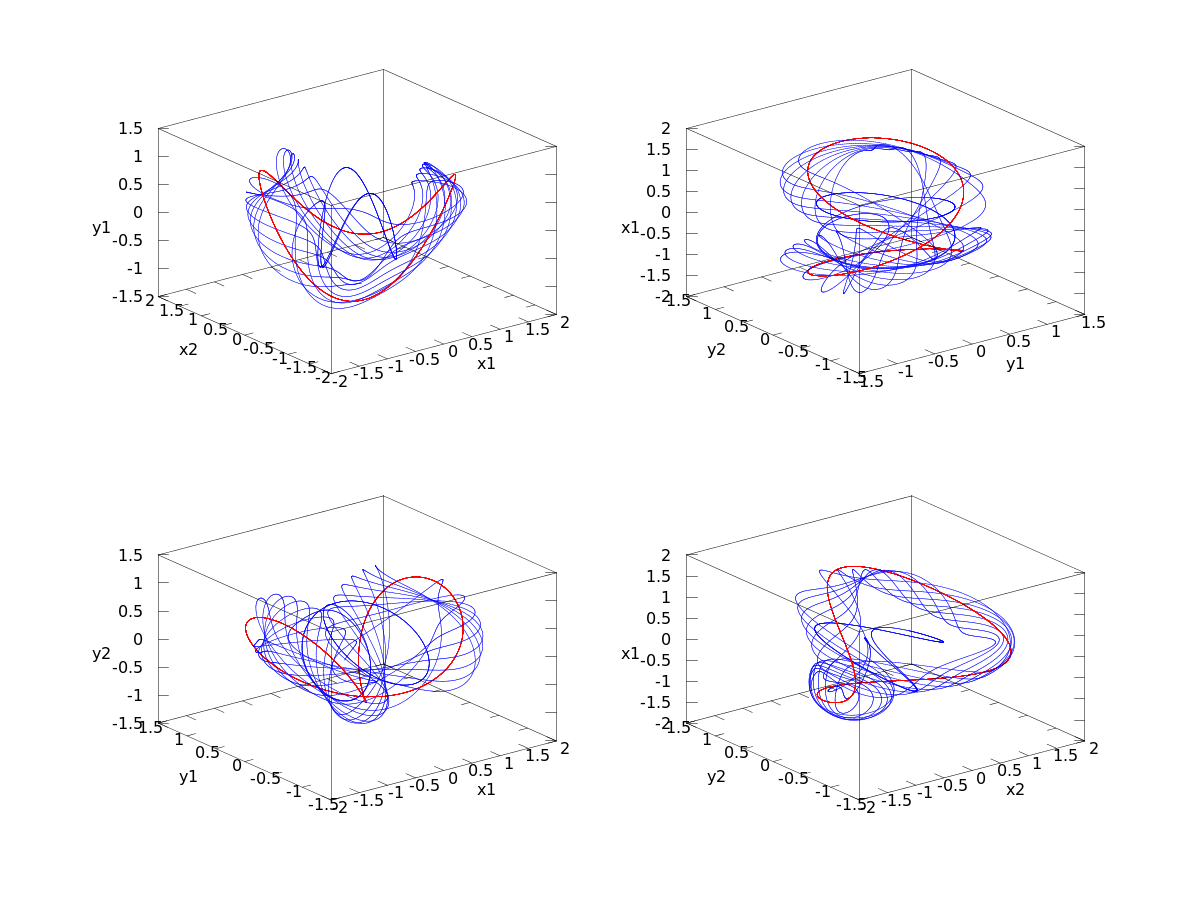
\includegraphics[width=0.9\textwidth]{BBpars3PKflow}
  \end{center}
  \caption{$3D$ projections of trajectories of \twoMode\ flow in full
  \statesp\ for parameters: $\mu_1 = 1.23436,\, a_1=-0.32304,\,
  b_1=-1.07444,\, c_1=1.00000,\, \mu_2=-0.23149,\, a_2=0.44110,\,
  b_2=-0.42287,\, c_2=-1.00000,\, e_2=0.67556$. Blue curve is a
  trajectory starting close to an unstable \reqv, the blue curve in the
  middle of the top left frame, which converges to a stable \rpo, better
  seen in \reffig{fig:BBpars3symmred}. This \rpo\ originates from a Hopf
  bifurcation of a \reqv, here the coexisting attractive \reqv\ plotted
  as red curve.
  }
  \label{fig:BBpars3PKflow}
\end{figure}

\item[2013-08-08  Burak]
According to my simulations, an attracting \eqv\ in the invariant
polynomials basis corresponds to a stable \reqv\ in the full \statesp.
({\bf [2013-08-13 Predrag]} correct.)
Eliminating these parameter values
gives more interesting dynamics.

\item[2013-08-13 Predrag] \refFig{fig:BBpars3PKflow} does not look like a
strange attractor. You really want to plot these things in $\{u,v,w,q\}$
representation first, and if something looks chaotic, look at it in a
Poincar\'e section; there it is much easier to see whether there is a
stretch \&\ fold unstable manifold with fractal structure.

\item[2013-08-14 Burak] I am going to try to compute Poincar\'e
sections and return maps tomorrow. I have to go back a little bit
since my existing Poincare\'e section codes for ChaosBook exercises
are extremely sloppy.

        \PCedit{
\item[2013-08-20 Predrag] You probably want to implement the
\HREF{http://www.streamsound.dk/book1/chaos/chaos.html\#82} {H\'enon trick},
ChaosBook section {\em 3.2 Computing a Poincar\'e section}.
        }

\item[2013-08-19 Burak] Took longer than I thought. I have the
\twoMode flow in invariant polynomials basis
(\reffig{fig:BBpars4invspacePKflow}), Poincar\'e section and radial
return map (\reffig{fig:BBpars4psectnretmap}). Convergence to a
periodic orbit is clearly seen on these plots, points with $r=6.8$
mapped on themselves.


\SFIG{BBpars4invspacePKflow}{}{
  A projection of \twoMode\ dynamics in the invariant polynomials basis
  $\{u,v,w,q\}$. Parameters: $\mu_1 =
  1.23436,\,a_1=-0.32304,\,b_1=-1.07444,\,c_1=1.00000,\,
  \mu_2=-0.23149,\,a_2=0.44110,\,b_2=-0.42287,\,
  c_2=-1.00000,\,e_2=0.67556\,.$
  }{fig:BBpars4invspacePKflow}

\begin{figure}%[ht]
  \begin{center}
  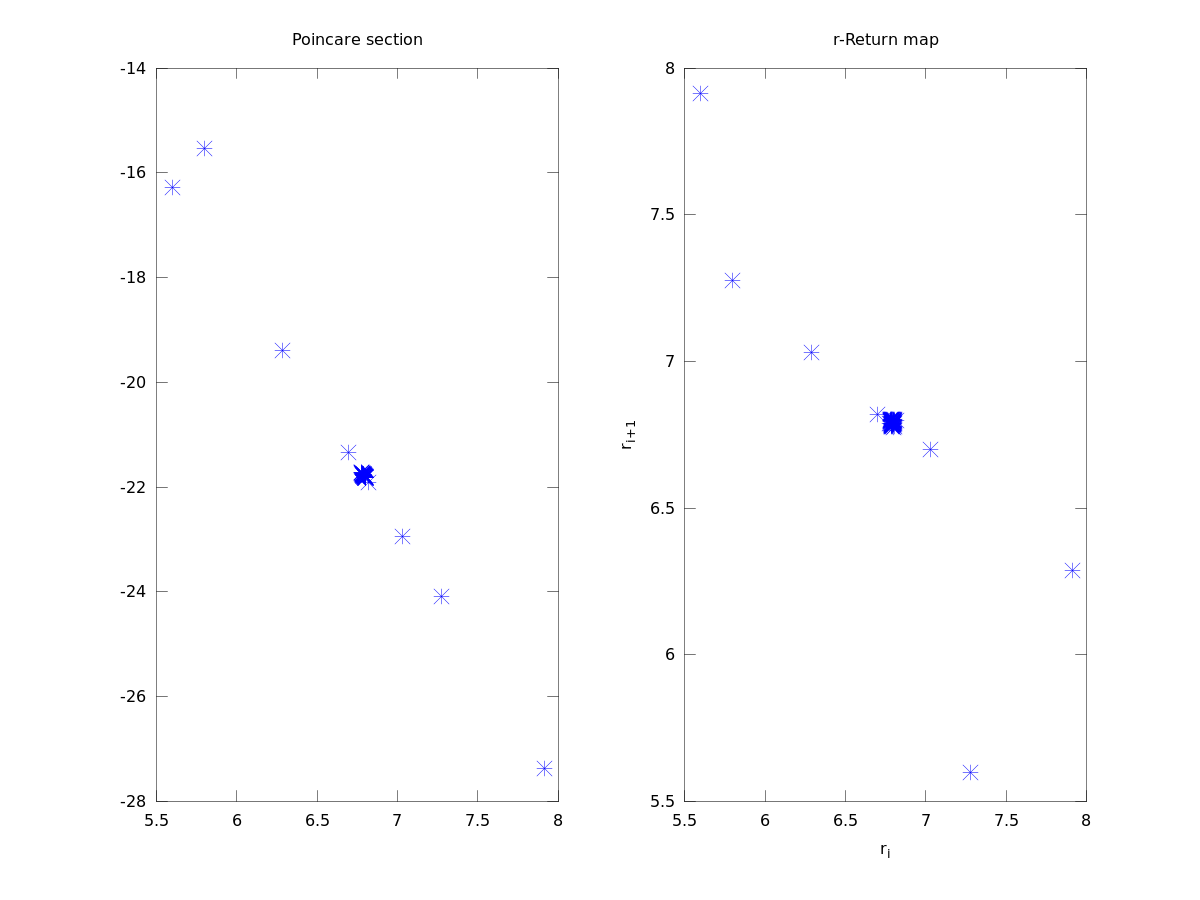
\includegraphics[width=0.9\textwidth]{BBpars4psectnretmap}
  \end{center}
  \caption{Left: Poincar\'e section for the \twoMode\ flow shown in
  \reffig{fig:BBpars4invspacePKflow}. Section hyperplane passes
  through $\sspRed = (u=10, v=6, w=0, q=0)$ and the plane normal is
  $\hat{n} = (-6,10,0,0)$ ($\sspRed$ rotated 90 degrees about $w$
  axis). Right: Poincar\'e return map of radial distance from $w$
  axis.}
  \label{fig:BBpars4psectnretmap}
\end{figure}

        \PCedit{
\item[2013-08-20 Predrag]
Looks right - you are converging to a limit cycle with a negative
least contracting Floquet multiplier. For limit cycles Poincar\'e
sections are boring, they will be useful only one you are looking at
strange attractors.
(I have, experimentally, commented your commit on gitHub, but that
looks useless. Did gitHub alert you to the comment?)
Have you computed Floquet multipliers of this limit cycle? They should
give you the convergence rate exactly.

Now see whether you can pick a convenient parameter that moves one or
a pair of Floquet multipliers through 1 and on to chaos.

As explained in
\HREF{http://www.streamsound.dk/book1/chaos/chaos.html\#78}
{ChaosBook}, 1\dmn\ Poincar\'e return maps, such as of
the radial distance from $w$ axis in \reffig{fig:BBpars4psectnretmap}
are misleading.
        }
\BBedit{
\item[2013-08-21]
I got notification for gitHub comment. I tried to calculate the Floquet multipliers but failed really badly at calculating the Jacobian. I thought that I could estimate the Jacobian (in the sense that it is defined in the ChaosBook, not like in Strogatz's book, I think his definition of Jacobian is the Stability Matrix of the ChaosBook) by multiplying the Jacobians for small time steps in a time ordered manner, but result was horrible. I think the numerical errors build up in an intolerable way. Can you refer me some paper/thesis/book that describes the correct way of computing this? I'm assuming that someone did this before and I'd rather not to re-discover it.
}

\begin{figure}%[ht]
  \begin{center}
  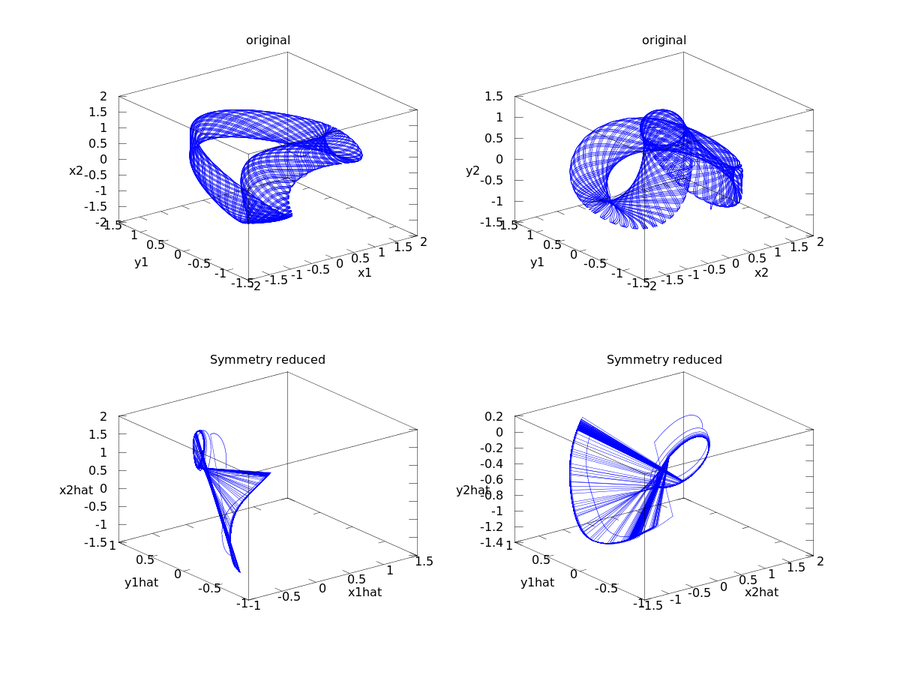
\includegraphics[width=0.9\textwidth]{BBpars3symmred}
  \end{center}
  \caption{Projections of \twoMode\ dynamics in full \statesp\ and symmetry reduced space. Parameters: $\mu_1 = 1.23436,\,a_1=-0.32304,\,b_1=-1.07444,\,c_1=1.00000,\,\mu_2=-0.23149,\,a_2=0.44110,\,b_2=-0.42287,\,c_2=-1.00000,\,e_2=0.67556$}.
  \label{fig:BBpars3symmred}
\end{figure}

\item[2013-08-08  Burak] I think this one (\reffig{fig:BBpars4PKflow}) is chaotic.

\begin{figure}%[ht]
  \begin{center}
  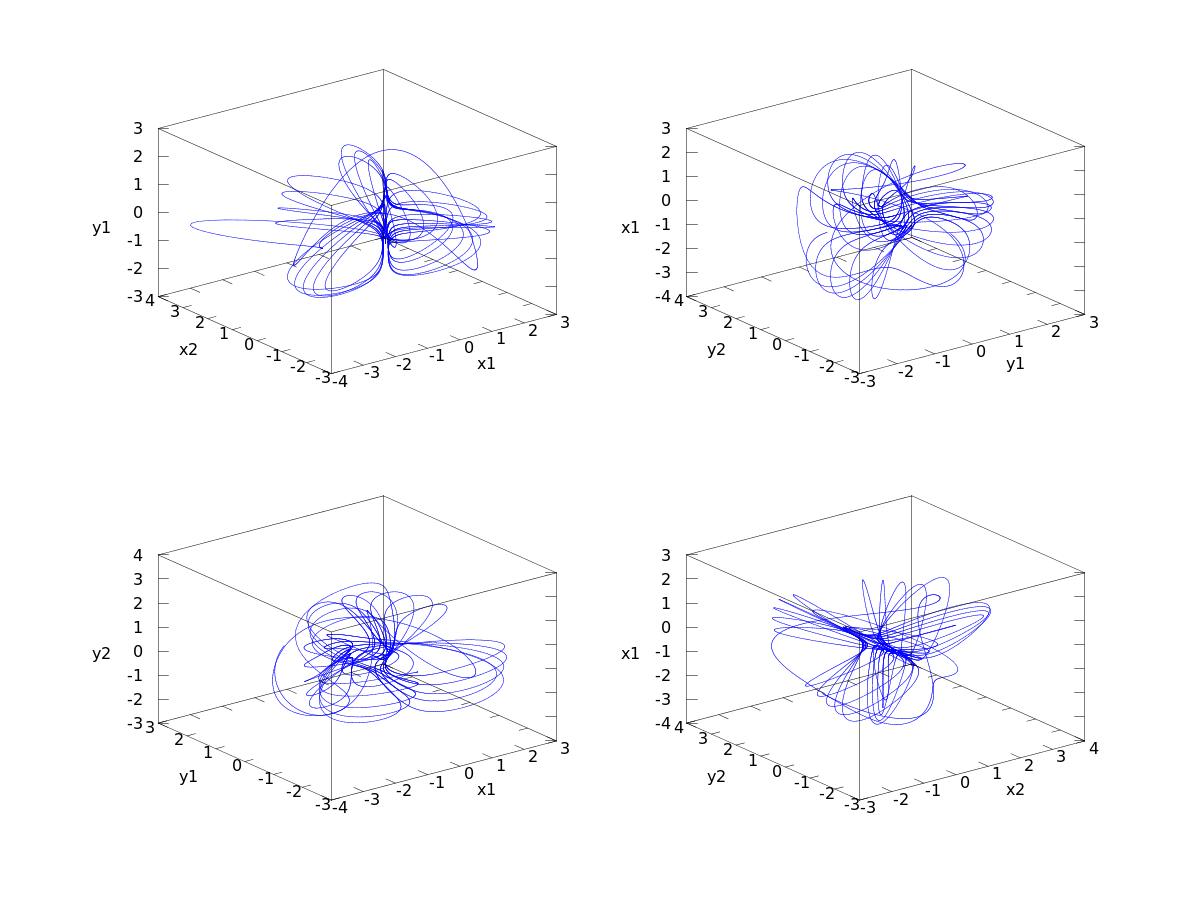
\includegraphics[width=0.9\textwidth]{BBpars4PKflow}
  \end{center}
  \caption{$3D$ projections of trajectories of \twoMode\ flow in full \statesp\ for parameters: $\mu_1 = 1.768907,\,a_1=0.406357,\,b_1=-1.660768,\,c_1=1.00000,\,\mu_2=-0.675565,\,a_2=0.083130,\,b_2=-0.047035,\,c_2=-1.00000,\,e_2=-0.455152$}.
  \label{fig:BBpars4PKflow}
\end{figure}

\item[2013-08-10  Predrag] I think you should cheat and find chaos
    first in the invariant polynomials basis $\{u,v,w,q\}$ -
    that is already symmetry reduced. After it looks chaotic in the
    invariant polynomials basis, plot the same trajectory in the equivariant
 $\pS = \{x_1,x_2,y_1,y_2\}$ coordinates. That should look messy. After
that construct a \slice\ $\pSRed$.
    \PCedit{
Examples are \reffig{fig:dangelmayrChaos} and \reffig{fig:dangelmayrChaos2}.
    }

That might sound masochistic (why not slice from the start?), but we
are only learning how to slice, and it is easier when you already have a
symmetry-reduced representation. For very high\dmn\ flows we will
not have the luxury of an invariant polynomials basis.

\item[2013-08-12  Burak] I got the parameters that I used in \reffig{fig:BBpars4PKflow} by generating random parameters, discarding if there are attractive equilibria or the time evolution is convergent or divergent in invariant polynomials basis. Unfortunately, this one was a periodic orbit in the invariant polynomials basis.

I added another criteria in my parameter generating code on Saturday to eliminate periodic orbits and discovered a bug in it later today. I spent most of today on varying parameters one by one and trying to see if those variations breaks that periodicity. I didn't get anything interesting yet.

I will run another 'new parameter set finder' tonight with the working periodic orbit elimination.

\item[2013-08-13 Predrag] One way to diagnose chaos  is to pick a stable
solution (like \reffig{fig:PKperorb}) and follow it as it undergoes a
Hopf bifurcation into a stable limit cycle. Then one keeps changing
parameters until this \po\ goes unstable and begets chaos, through period
doublings and beyond. To do this, you need to be able to compute Floquet
multipliers of your invariant solutions. For example, does the unstable
\rpo\ in \reffig{fig:BBpars3PKflow} have complex pair of multipliers
(underwent a Hopf bifurcation that turned it unstable) or two real
multipliers (perhaps on the way to period doubling sequence?)

\item[2013-08-13 Predrag] I have asked a Geophysical Fluid Dynamics
(Woods Hole) Fellow Yuuki Yasuda (Earth and Planetary Science, U. Tokyo,
yyuuki@eps.s.u-tokyo.ac.jp) to learn how to use
\HREF{http://sourceforge.net/projects/auto-07p/} {AUTO}, for the same
reason - to follow bifurcations of initially invariant solutions, see how
they go into chaotic behavior. It is well written code which I think is
only good in small dimensions, so we have not used it for our high\dmn\
hydrodynamics calculations. Yuuki will report to me today how it is
working; I'll report whether it might be useful to you.

\item[2013-08-13 Predrag]
I keep getting confused about whether you are plotting a \reqv\ or a \po,
and as we will need this anyhow, please define \eqv, \reqv, \po, and
\rpo\ in \refsect{chap:2modesBBproj}, just to be sure we are on the same
page. (I keep using macros for their names, because depending on the
publication and audience, a `\reqv' might be called a `rotating wave',
etc.)

\end{description}

\noindent{\bf A truncation of PDE representations:}
The {\twoMode} system is the simplest, coarsest example of a truncation
of a Fourier representation of a PDEe. Consider, for example, the $1D$
\KSe.
%
\PC{2013-08-13 Predrag copied this from \refref{SCD07}, to set up
the conventions for the \KSe\ calculations.}
%
The time evolution of the `flame front velocity'
$u=u(x,t)$ on a periodic domain $u(x,t) = u(x+L,t)$ is given by
\beq
  u_t = F(u) = -{\textstyle\frac{1}{2}}(u^2)_x-u_{xx}-u_{xxxx}
    \,,\qquad   x \in [-L/2,L/2]
    \,.
\ee{BBks}
Here $t \geq 0$ is the time, and $x$ is the spatial coordinate.
The subscripts $x$ and $t$ denote partial derivatives with respect to
$x$ and $t$. In what follows
we shall state results of all calculations either in units of the
`dimensionless system size' $\tildeL$, or the system size $L = 2 \pi
\tildeL$. All numerical results presented in this report
are for $\tildeL=22/2\pi \simeq 3.5014$.
Spatial periodicity $u(x,t)=u(x+L,t)$
makes it convenient to work in the Fourier space,
\beq
  u(x,t)=\sum_{k=-\infty}^{+\infty} a_k (t) e^{ i k x /\tildeL }
\,,
\ee{BBeq:ksexp}
with the $1$-dimensional PDE \refeq{BBks}
replaced by an infinite set of
ODEs for the complex Fourier coefficients $a_k(t)$:
\beq
\dot{a}_k= \pVeloc_k(a)
     = ( q_k^2 - q_k^4 )\, a_k
    - i \frac{q_k}{2} \sum_{m=-\infty}^{+\infty} a_m a_{k-m}
\,,
\ee{BBexpan}
where $q_k = k/\tildeL$.
Since $u(x,t)$ is real, $a_k=a_{-k}^\ast$, and we can replace the
sum by a $k > 0$ sum. In the {\twoMode} system we keep only the
$k \in \{\pm 1,pm 2\}$ terms. This is very wrong as an approximation to
the \KSe, but --in the spirit of the Lorentz equations-- OK for hoping
to learn something about the qualitative dynamics of this class of
PDEs.

\begin{description}

\item[2013-08-13 Predrag]
A problem with {\twoMode} system is too many parameters (seven! - see
\refeq{PKinvEqs5b}). How about reducing the number of parameters by
demanding that our {\twoMode} system is the $k \in \{\pm 1,\pm 2\}$
truncation of \KS? There is only one parameter left (the system size
$L$), so that is probably too radical -- maybe it will
yield no interesting dynamics at all,
but let something physical like this guide you in reducing the number of
parameters.

The physical setting is that a dissipative turbulent system has a finite
number of Fourier modes nonlinearly coupled and of comparable amplitudes,
while high modes are very strongly suppressed by dissipative terms like
$q_k^4$ in \refeq{BBexpan}. (Xiong Ding can explain the `physical
dimension' to you). So you will be interested in chaotic solutions for
which the two modes $u = {z}_1 \overline{z}_1,\, v = {z}_2
\overline{z}_2$ in \refeq{PKinvEqs1} are of comparable magnitude.

One good exercise is to go through Ruslan's {\em 15.7.1 2009-08-26
Epicycles: 2-Fourier modes} in the \HREF{../blog/blog.pdf} {main blog}.
In this model he looks at a trivial dynamics of two uncoupled modes. I do
not agree with Ruslan pessimistic conclusion - search for `epicycles'
within the blog for more optimistic angles.

\item[2013-08-30 Burak]
I computed dynamics of two mode truncation of $1D$ \KSe\ and found
nothing interesting. Solutions either diverges or converges to the
origin. Mathematica files where I derived the velocity functions and
stability matrices, along with the Matlab files for numerical work
are in
\\
\texttt{/blog/burak/2modeKuramotoShivashinski}.


\item[2013-08-21 Burak] I varied the parameters I used in \reffig{fig:BBpars4invspacePKflow} and \reffig{fig:BBpars4psectnretmap} and
the \fixedpnt\ in the Poincar\'e section (attracting limit cycle in the flow) got bifurcated to a two cycle. After playing a little bit more, I got \reffig{fig:BBinvspacePKflow130821}. In \reffig{fig:BBinvspacePKflow130821}, every trajectory goes near the origin, make a small turn there and start go away and make another turn at a different location far away from the origin and go back. This behavior is better seen in the Poincar\'e return map on the right hand side of \reffig{fig:BBpsectandretmap130821}. On the return map, different points with larger radial distances are mapped to the neighborhood of the radius 5, and points with radii close to 5 are mapped to different points (without following a regular pattern.). This, I think, satisfies the `extreme dependence on initial state' condition of chaos.

\SFIG{BBinvspacePKflow130821}{}{
  A projection of \twoMode\ dynamics in the invariant polynomials basis
  $\{u,v,w,q\}$. Parameters: $\mu_1 =
  1.23436,\,a_1=-0.32304,\,b_1=-1.07444,\,c_1=1.00000,\,
  \mu_2=-0.23149,\,a_2=0.44110,\,b_2=-0.42287,\,
  c_2=-1.00000,\,e_2=1.8\,.$
  }{fig:BBinvspacePKflow130821}

\begin{figure}%[ht]
  \begin{center}
  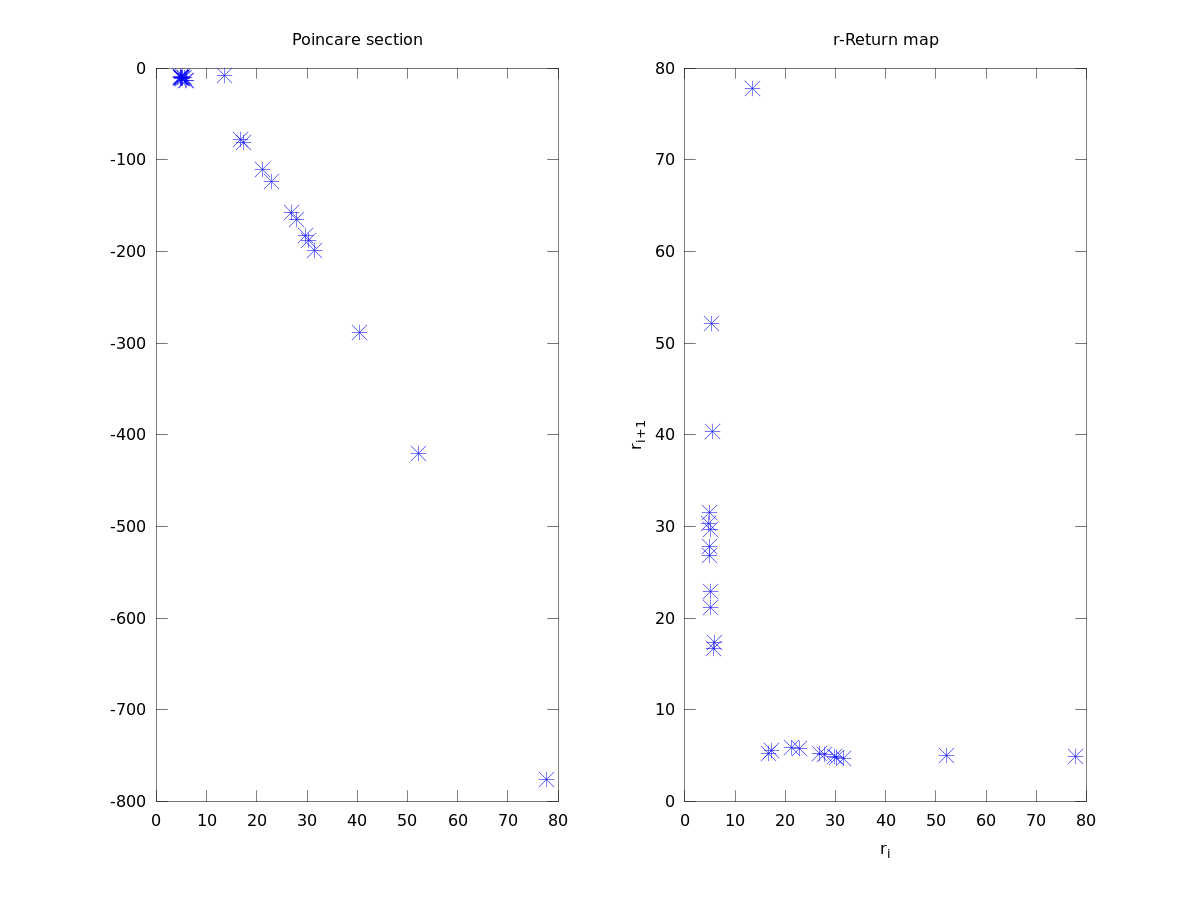
\includegraphics[width=0.9\textwidth]{BBpsectandretmap130821}
  \end{center}
  \caption{Left: Poincar\'e section for the \twoMode\ flow shown in
  \reffig{fig:BBinvspacePKflow130821}. Section hyperplane passes
  through $\{u,v,w,q\} = \{10, 4, 0, 0\}$ and the plane normal is
  $\hat{n} = (-4,10,0,0)$ ($\{u,v,w,q\}$  point rotated 90 degrees about $w$
  axis). Right: Poincar\'e return map of radial distance from $w$
  axis.}
  \label{fig:BBpsectandretmap130821}
\end{figure}

After liking what I saw in the invariant polynomials basis, I went ahead and integrated the system in the full state space and try to \slice\ it using method of moving frames. One projection of the full \statesp\ flow is in \reffig{fig:BBfullspaceflow130821} and the \reffig{fig:BBsymmredflow130821} is how the symmetry-reduced \statesp\ looks like.
I tried a few template points (I tried to find \eqva\ and use them, didn't look good at all) and got the prettiest picture with the template $\slicep = (1,1,0,0)$.

\SFIG{BBfullspaceflow130821}{}{
  A projection of \twoMode\ dynamics in the full state space $\{x_1,x_2,y_1,y_2\}$. Parameters: $\mu_1 =
  1.23436,\,a_1=-0.32304,\,b_1=-1.07444,\,c_1=1.00000,\,
  \mu_2=-0.23149,\,a_2=0.44110,\,b_2=-0.42287,\,
  c_2=-1.00000,\,e_2=1.8\,.$
  }{fig:BBfullspaceflow130821}

 \SFIG{BBsymmredflow130821}{}{
  A projection of \twoMode\ dynamics of \reffig{fig:BBfullspaceflow130821} after symmetry reduction using the method of moving frames (post processing). Slice template: $\slicep = (1,1,0,0)$.
  }{fig:BBsymmredflow130821}

\item[2013-08-22 Predrag] This looks promising. Comparing
\reffig{fig:BBinvspacePKflow130821}
and
\reffig{fig:BBsymmredflow130821}
you can see one of the reasons why I do not like symmetry reduction by
slices to invariant polynomials basis, even in a few dimensions, where
syzygies are few: invariant polynomials scrunch everything into the
origin. If you and Daniel settle on this one as an example (I would
prefer an example where you need at least two slice hyper-planes -
presumably when the two modes are of comparable strength; and when
some parameters are eliminated by requiring that the \twoMode\ system
is close to the \KS\ 2-mode truncation), than you should do
Poincar\'e sections more carefully, using points ant not '*',
constructing the unstable manifolds by continuing the Floquet vectors
of the initial (now unstable) Hopf cycle, and constructing the return
map from them, as discussed in
\HREF{http://www.streamsound.dk/book1/chaos/chaos.html\#260/z}
{Chapter 12} {\em Stretch, fold, prune}.

\item[2013-08-21 Daniel] Ok... so while you guys are off doing all the thinking, I brute forced a set of parameters that appear to give chaotic dynamics. Basically, I used the same Monte Carlo-ish technique that I used to find ``good'' templates for slicing \CLf where I let the computer vary parameters by a little bit and see if they give better results. If so they are used a new starting point and the calculation is repeated; if not they are discarded. To measure ``success'' I calculated finite time Lyapunov exponents for the \twoMode\ system in the invariant polynomials basis and required that the leading one be positive (the more positive the better), the second one be zero (guaranteed by autonomous dynamics), and the third one be negative (the more negative the better). The algorithm prints them out in order, so the fourth one is automatically more negative than the third. The code I used is in \texttt{/cgang/Daniel/Matlab/ChaoticExponentsCalculation} and should have enough comments for intelligibility. The algorithm used is based on Wolf et al. \cite{WolfSwift85}. I let the computer run this for a day or so and got the following set of parameters:
\bea
\mu_1&=&-2.8023, \mu_2=0.6128, a_1=-0.9146, a_2=-2.6636
    \continue
b_1  &=& -0.6141, b_2=-0.0144, c_1=-4.1122, c_2=1.8854, e_2=2.1769
\,.
\label{eq:PKChaoticParams}
\eea

\item[2013-08-23 Predrag to Daniel]
Got your rotatable Matlab file  - it was probably OK yesterday, I
just did something wrong then....

It's both a boring looking attractor (this is is really in a single
slice hyperplane coordinates; not the invariant polynomials basis?),
and a little bit too singular - maybe two charts needed?

\item[2012-08-25 Daniel to Predrag] I might have had the axis
labels wrong in the Matlab fig that I sent you. Basically in
invariant coordinates it looks like \reffig{fig:PKChaoticInv} and in
Cartesian coordinates it looks like \reffig{fig:PKChaotic}.

\item[2013-08-21 Daniel]
Calculating the Lyapunov exponents for the \twoMode\ system using the parameters from \refeq{eq:PKChaoticParams} gives
\beq
\{\lambda_i\} =\{\lambda_i\} = \{0.09,\, 0.00,\, -9.14,\,-17.77\}
\,.
\ee{eq:PKLyapunovExp}

\item[2013-08-23 Predrag to Daniel]
are these the
\HREF{http://www.streamsound.dk/book1/chaos/chaos.html\#137/z}
{Lyapunov} exponents, or the real parts of stability exponents?
I guess it is
Lyapunov exponents. Ask Xiong to compute stability exponents for
this system - while finite time stability and Lyapunov exponents
differ, I do not know whether they really converge to each other for
long times. You are really able to compute
$ \lambda_4=-17.77$ to even one digit, let alone 4 digits?


\item[2013-08-25 Daniel to Predrag]             \toCB
Well Wolf \etal\rf{WolfSwift85} call them Lyapunov exponents in the
paper where the algorithm that I used is described. I don't know that
I would necessarily trust the -17.77 to any precision but it is what
the code spits out. It does spit out the REALLY negative Lyapunov
exponent for the Lorenz system (-22.46) that is reported in the
literature\rf{WolfSwift85,Briggs1990}, as well as the -9.77
that is reported for R\"ossler to within 0.1, so while maybe I
wouldn't swear that the fractional part is correct, I think the -17
is probably reliable.

\item[2013-08-25 Predrag]
That's a copout. I gave you the link
(\HREF{http://www.streamsound.dk/book1/chaos/chaos.html\#137/z}
{\emph{Lyapunov}} \emph{exponents}) because the literature is totally
confused, and describes two different things by the same name. I
believe that covariant vectors and the corresponding multipliers are
the correct object, Lyapunov exponents are not the right thing. If
you read the description of their algorithm you will know what they
are computing, so do check that. My collaborators were never able to
compute very negative stability and/or Floquet exponents accurately
(if at all), but the algorithm of Ginelli \etal\rf{GiChLiPo12} that
Xiong should implement is supposed to compute \emph{all} to machine
precision.
    \PCedit{
So once you have some exponents you think are worth
checking, ask Xiong to check his algorithm against yours. Being a
classical graduate student, Xiong has so far refused to work on
anything less than the 32\dmn\ \KS\ system.
    }

\item[2013-08-25 Daniel to Predrag]Ok... so looked at the Wolf et al. paper more carefully. I'm
pretty sure it's Lyapunov exponents. I know they are a relic of the 80's and
not endorsed by Das Buch, but I was only using them to try and find
parameters that would give us chaotic behavior. I just know that the leading exponent is positive, the
second one is within 0.001 of zero, and the third and fourth ones are negative. I'll
stop by to discuss tomorrow just to make sure.

\item[2013-08-21 Daniel]
Coincidentally, the first three are almost exactly the Lyapunov
exponents for the R\"ossler system ($\lambda_1=0.09,
\lambda_2=0.00,\, \mathrm{and}\, \lambda_3=-9.77$).
\refFig{fig:PKChaoticInv} shows what it ends up looking like in the
invariant polynomials basis. If you run it longer it just fills out
the attractor. \refFig{fig:PKChaotic} shows it in the full
\statesp. If you run it longer it just fills out the attractor.

\item[2013-08-23 Burak] I integrated the system with Daniel's parameters and my simulation converged to \eqv\ $(0,425.56,0,0)$ in the invariant polynomials basis
\BBedit{(see \reffig{fig:BBPKflowDanielPars}\,(a))}. I found all eigenvalues of the stability matrix at this point to be negative with zero imaginary parts. As I expected, this resulted in a \reqv\ in the full state space
\BBedit{(see \reffig{fig:BBPKflowDanielPars}\,(b))}.

I also sliced this solution with the same template that I used for my
parameters and got \reffig{fig:BBsymmredPKDanielPars0t12} for the
time that the solution looked chaotic (t from 0 to 12), it then makes
a jump (see \reffig{fig:BBsymmredPKDanielPars14t20} (a) for evolution
from t=14 to t=17) as the solution in invariant polynomials basis
does, and then converges to the \reqv\ (see
\reffig{fig:BBsymmredPKDanielPars14t20} (b) for evolution from t=15.5
to t=20) by going through a spiral.
    \PCedit{what figure does  fig:BBsymmredPKDanielPars14t20 refer to?
    If it was erroneous, rewrite this post; also all other figures
    that have turned to ?'s now. Whenever you comment out / remove / rename
     a labeled environment,
    search for the commented-out label and fix all references to it.}
I'm blogging this because I found
it interesting to see a ``spiral in'' type of convergence on the
symmetry reduced manifold while all eigenvalues of the stability
matrix of the \eqv\ in the invariant space have zero imaginary
parts.

\item[2013-08-23 Predrag] Having \eqv\ at $(0,425.56,0,0)$ in the
invariant polynomials basis must mean that it sits in an invariant
subspace (there is much discussion of a such subspace earlier in the
blog, check whether it is in this subspace). Then it will have
eigenvectors within the subspace, and others that point out - all of
that should be significant. `Spiral in' I find unexpected, maybe
there is an unstable \eqv\ you are missing?

\item[2013-08-23 Burak]
The inconsistent look of the equilibria was due to a numerical error.
I used different time steps for simulations in invariant basis
($\Delta t = 0.001$) and full state space ($\Delta t = 0.01$). When I
checked in the invariant polynomials basis, I found that when I use
the smaller time step, simulation converges to a \reqv\
(zero velocity) but if I use the bigger time step, it ends up in a
\po. I calculated the final point of the full state space
simulation and found a point corresponding to the cycle in the
invariant polynomial space.
({\bf [2013-08-24 Predrag]} Do you mean: ``I calculated the
\reqv\ in the full \statesp\ and found the corresponding \eqv\  in
the invariant polynomials basis''?)({\bf [2013-08-25 Burak]} Yes.)
My point is, there is no direct correspondence between the invariant
polynomials basis plot that I posted (\reffig{fig:BBPKflowDanielPars}
(a)) and full \statesp\ plot (\reffig{fig:BBPKflowDanielPars} (b)).
Since symmetry reduction plots are generated from the full \statesp\
data, they are also not so accurate. I am now simulating the full
\statesp\ with higher resolution, I already found that the full
\statesp\ system converges to an \reqv\ in the $(y_1,y_2)$ plane and
$x_1 = x_2 = 0$ all the time. This is expected from the
transformation relations \refeq{eq:PKinvxirels} and all points on
this \reqv\ are mapped to the invariant polynomials basis \eqv\
$(0,425.56,0,0)$. Sliced results will be ready tomorrow morning.


\begin{figure}%[h]
	\centering
		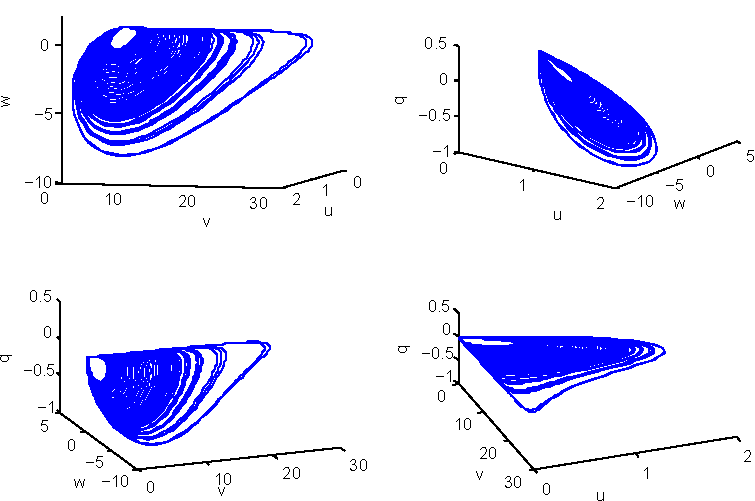
\includegraphics{PKChaotic}
	\caption{\twoMode\ system in invariant polynomials basis using
        parameters \refeq{eq:PKChaoticParams}.
        }
	\label{fig:PKChaoticInv}
\end{figure}

\begin{figure}%[h]
	\centering
		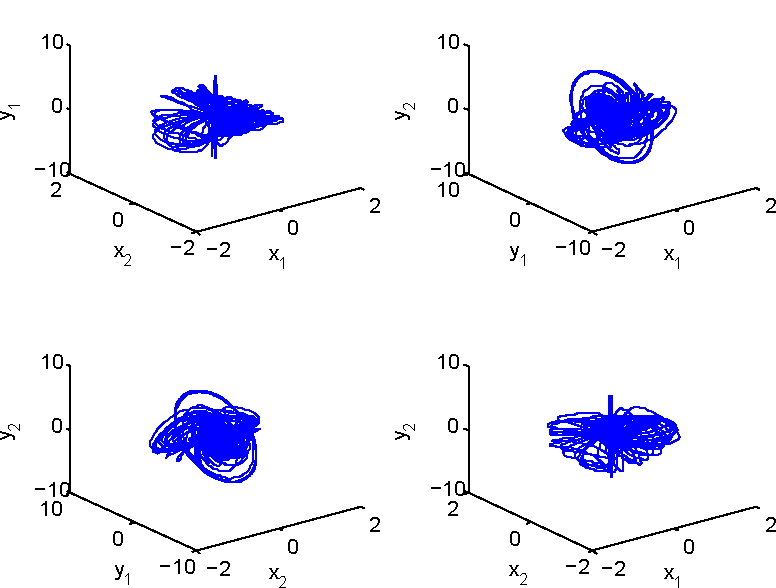
\includegraphics{PKChaotic2}
	\caption{\twoMode\ system in the full \statesp\
    ($x_1,x_2,y_1,y_2$) using parameter values
    \refeq{eq:PKChaoticParams}.}
    \label{fig:PKChaotic}
\end{figure}

\begin{figure}%[H]
\centering
 (a) 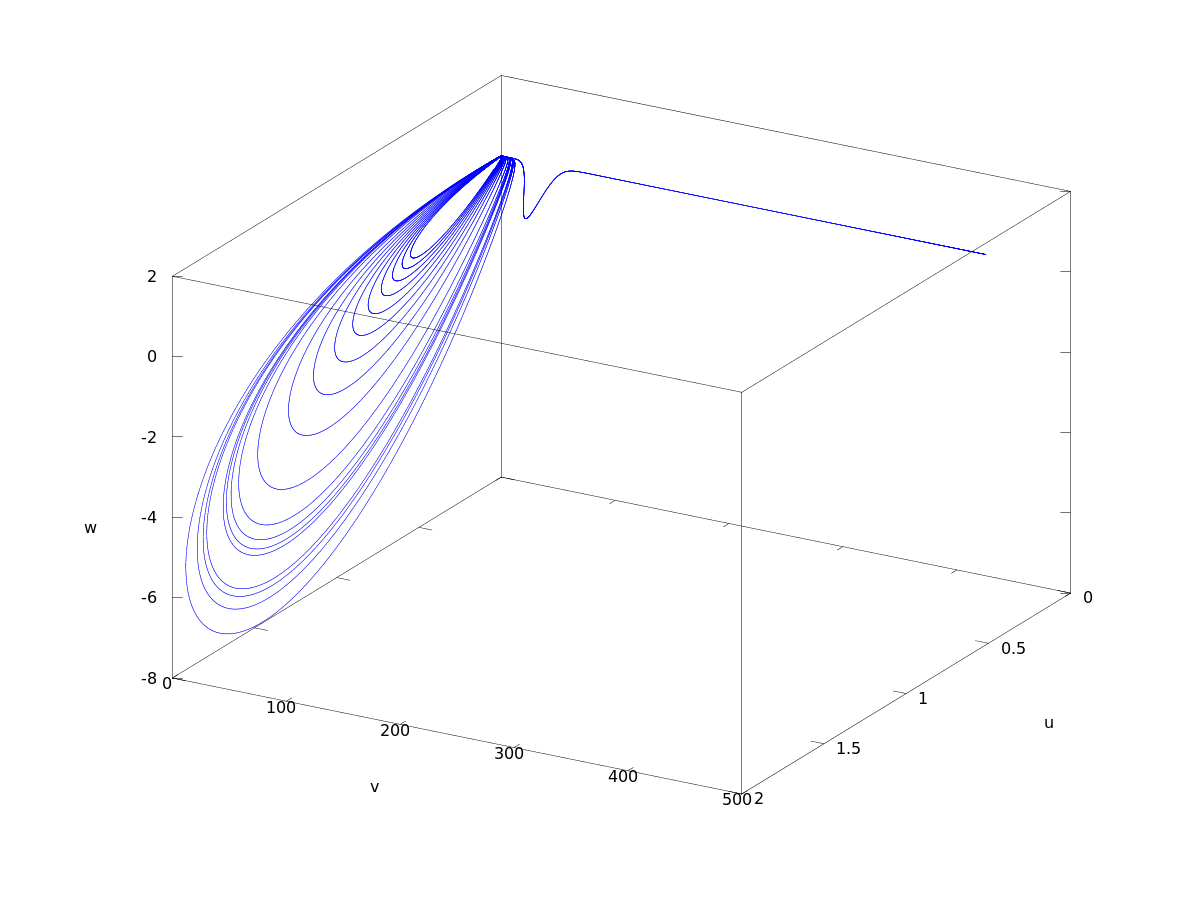
\includegraphics[width=0.35\textwidth]{BBinvspacePKflowDanielPars}
 (b) 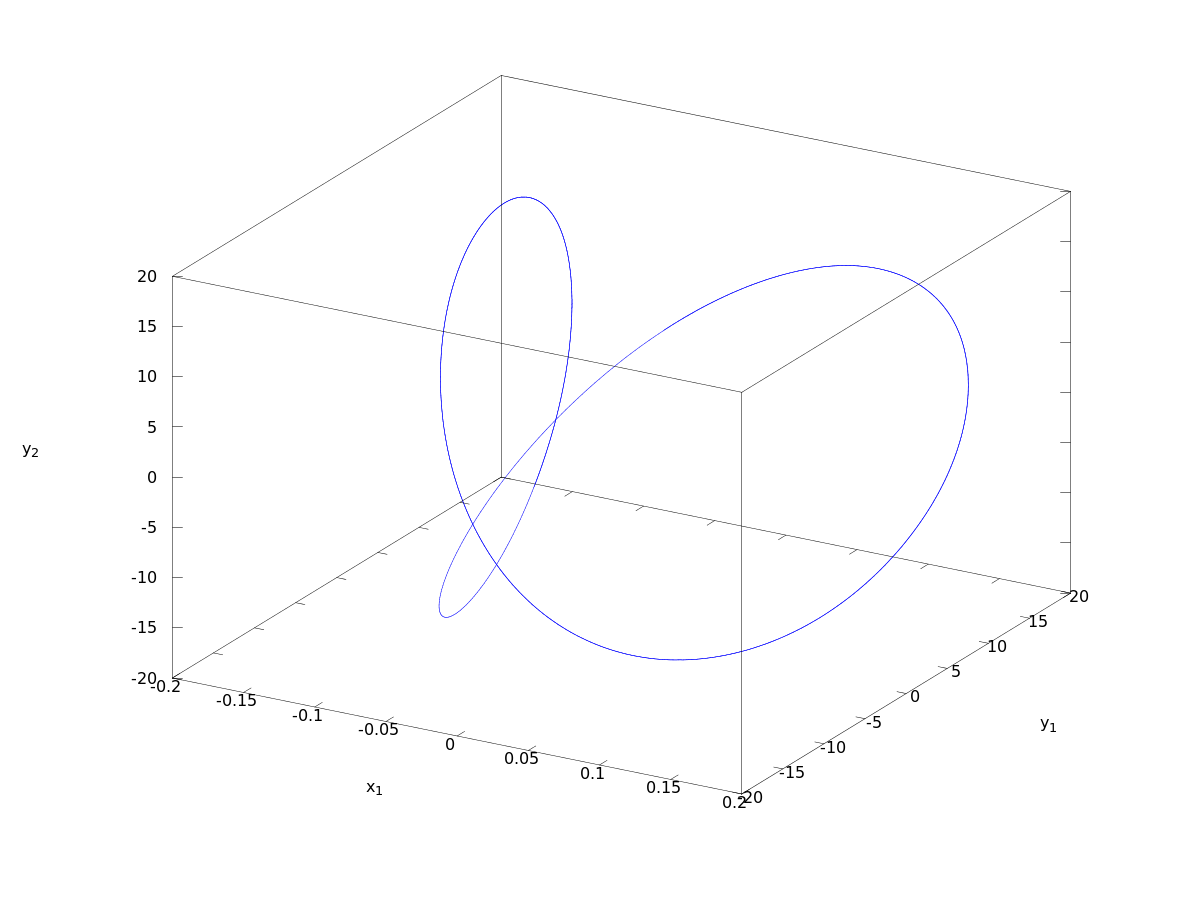
\includegraphics[width=0.35\textwidth]{BBreleqDanielPars}

\caption{(a) A projection of \twoMode\ dynamics in the invariant polynomials
  basis $\{u,v,w,q\}$, parameters given in \refeq{eq:PKChaoticParams}.
  (b) \Reqv\ in the full \statesp\ corresponding to the \eqv\ in (a).}
\label{fig:BBPKflowDanielPars}
\end{figure}

\SFIG{BBsymmredPKDanielPars0t12}{}{
  A projection of \twoMode\ dynamics of \reffig{fig:BBPKflowDanielPars} in
 a single slice hyperplane using the method of moving frames (post processing).
 A single template: $\slicep = (1,1,0,0)$.
}{fig:BBsymmredPKDanielPars0t12}

%\begin{figure}%[H]
%\centering
 %(a) 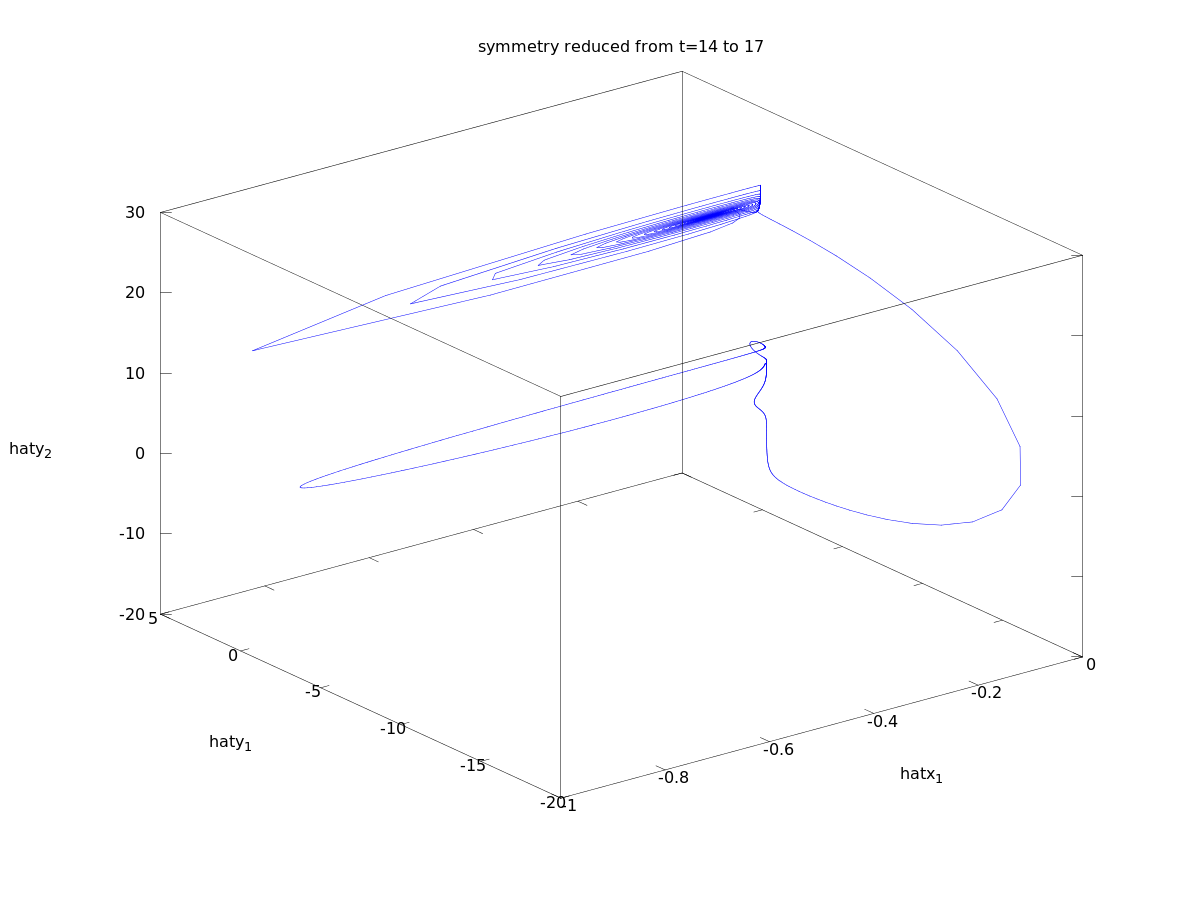
\includegraphics[width=0.35\textwidth]{BBsymmredPKDanielPars14t17}
 %(b) 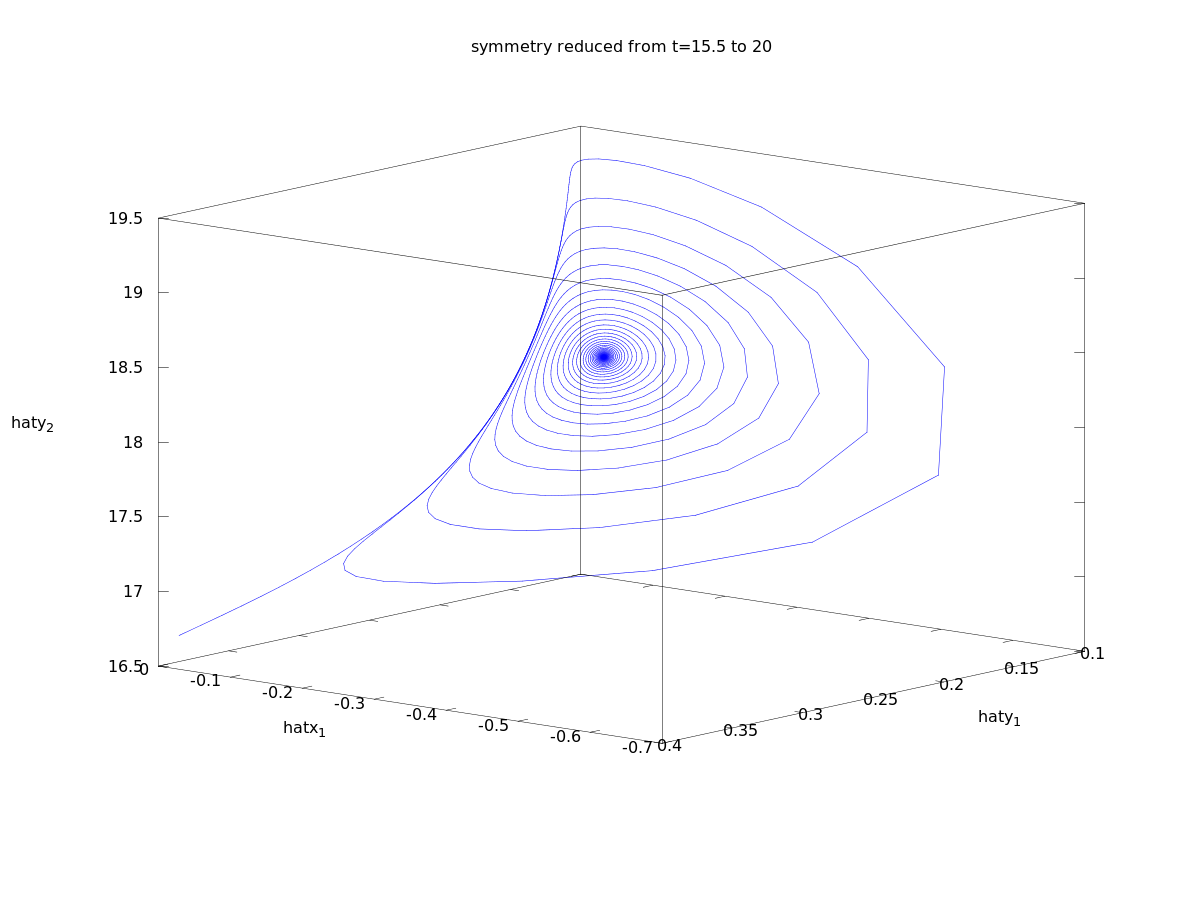
\includegraphics[width=0.35\textwidth]{BBsymmredPKDanielPars15p5t20}

%\caption{(a) Symmetry reduced \twoMode\ dynamics corresponding with parameters .
%(b) Spiral-in to \reqv\ in the full \statesp\ corresponding to the \eqv\ in (a).}
%\label{fig:BBsymmredPKDanielPars14t20}
%\end{figure}


\item[2013-08-23 Predrag]
% I cannot make sense of either \reffig{fig:BBsymmredPKDanielPars14t20}
% or its captions
\refFig{fig:BBsymmredPKDanielPars0t12} is cute.
Basically, you have to keep checking whether your trajectory has
crossed the border of your single slice hyperplane. If so, two-hyperplane (with a ridge
in-between) cover of the slice is needed.
%\item[2013-08-23 Burak] Sorry! I forgot to edit captions after
%copy/paste. I just wanted to show how the system converges to the
%relative equilibria on the reduced space by plotting different time
%intervals seperately. However, as I realized that I should have
%integrated the system with a smaller time step, these plots are
%irrelevant for now, hence, I commented them out. I will update them
%with meaningful captions hopefully tomorrow morning.


\item[2013-08-23 Daniel] Just ran a couple of hundred simulations
using the parameters from \refeq{eq:PKChaoticParams} with random
initial conditions taken from a Gaussian ball centered at
$(u,v,w,q)\, =\,(0,0,0,0)$ with radius of about 8. Each simulation
was run for 1\,000 time units. I found that the trajectories ended up
at Burak's \eqv\ about 70\% of the time, so it's basin of attraction
is definitely significant. Then again, 30\% of trajectories fall into
the chaotic attractor and stay there for long times, so it's basin of
attraction is not tiny either. It also doesn't seem like the chaotic
dynamics are transient. I can integrate out to 20\,000 time units and
still be in the attractor if I start in its basin of attraction
(e.g., $(u,v,w,q)\, =\,(1,1,1,1)$ . Maybe we can tweak the parameters
to make Burak's \eqv\ unstable or hyperbolic? Looking at the
symbolic expressions for the eigenvalues, I don't see a particularly
obvious way to do this. The expressions are a mess!

\item[2013-08-23 Predrag] I do not mind coexisting attractors - that's what we have
for the pipe and the \pCf s anyway.

\item[2013-08-23 Burak] I tried to calculate the dynamics within the slice and then reconstruct today. It worked perfectly on 1 slice for Daniel's parameters. I am commiting the Matlab (Octave) functions and scripts that I used at
\texttt{/blog/burak/PorterKnobloch}
If you want to test them, first run \texttt{generator.m}, this will generate generator.mat with the group generator matrix in it. You can then integrate the system by running \texttt{PKintegrate.m} and then you can reduce the symmetry by running \texttt{PKComputeMovingFrames.m} and you can do everything starting from the reduced space by running \texttt{PKComputeDynamicsWithinSlice.m}. Now to compare the results from both approaches you can run \texttt{PKPlotDynamicsWithinSlice.m}. You should see exactly the same dynamics on the slice and in the full state space calculated with different techniques. I am not posting these results but basically I get the exact same plot with \reffig{fig:BBsymmredPKDanielPars0t12} by calculating the dynamics entirely on the slice.

I was not this lucky with my parameters. When I tried to simulate the dynamics on the slice with the same initial point, I got something that started similar to the slice from the moving frames, and then settled on a limit cycle, results of two methods are side by side on \reffig{fig:BBreduceddynamicstwomethods} for comparison. I also plotted the variation of the group parameters, $\phi(t)$ (computed within the slice) and $\phi(\tau)$ computed using moving frames, and the square of the Euclidian norm of the difference between state vectors, $|x_r(t)-x(t)|^2$, calculated both by reconstruction from the slice and the direct integration in the full \statesp\ (\reffig{fig:BBreductionmethodsdiff}). Any ideas why is this the case?

\begin{figure}%[ht]
  \begin{center}
  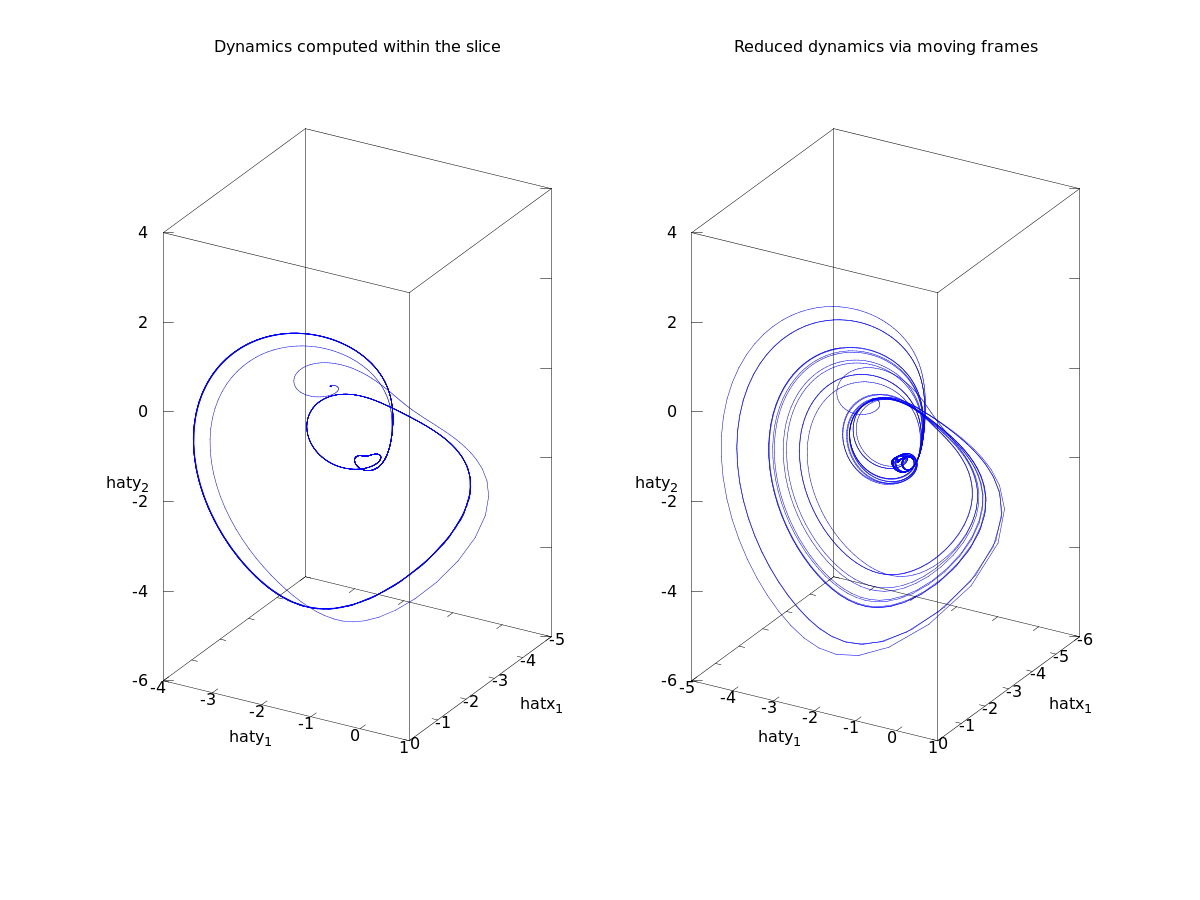
\includegraphics[width=0.9\textwidth]{BBreduceddynamicstwomethods}
  \end{center}
  \caption{Left: Dynamics of \twoMode\ system with the parameter set used
    in \reffig{fig:BBfullspaceflow130821} computed within the slice with
    the template $\slicep = (1,1,0,0)$. Right: Symmetry reduced dynamics
    of \twoMode\ system with the parameter set
    used in \reffig{fig:BBfullspaceflow130821}
    computed using Moving Frames Method. \textbf{ES:} Is the trajectory
    in both panels the same? Is the integration time longer in the second case?
    I don't understand why there is difference between the two figures if the
    template is the same. \textbf{BB:} I believe this is due to a numerical error resulting from the trajectory passing close to the chart border. I did not check this one specifically, but I observed a similar situation today and found out that this was the case. Please see my discussion in [2013-09-14 Burak].
     }
  \label{fig:BBreduceddynamicstwomethods}
\end{figure}

\begin{figure}%[ht]
  \begin{center}
  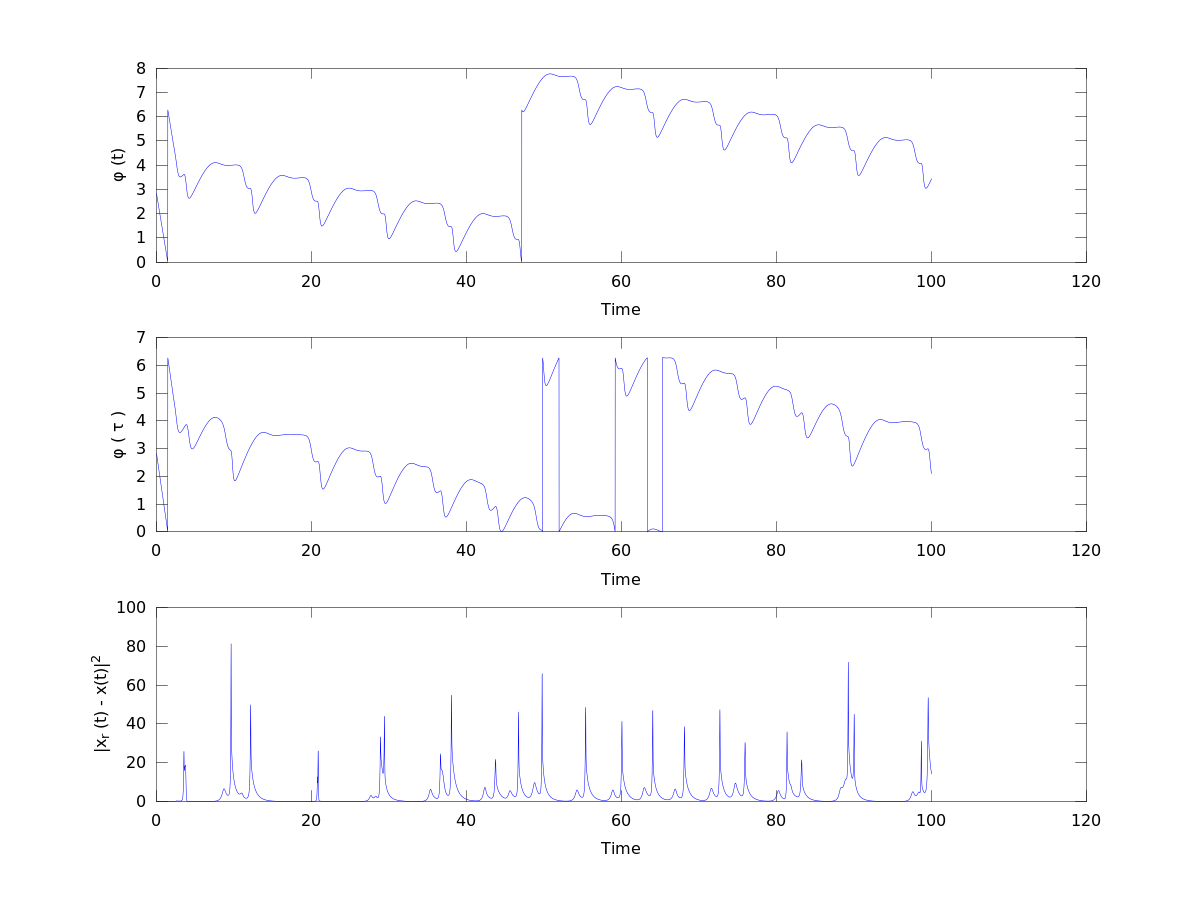
\includegraphics[width=0.9\textwidth]{BBreductionmethodsdiff}
  \end{center}
  \caption{
  [Top] Group parameter versus time obtained from the computation of
  dynamics within the slice. [Middle] Group parameter versus time
  obtained from the moving frames calculations. [Bottom] Square of
  the Euclidian norm of the difference between state vectors
  calculated both ways. The same parameters as in
  \reffig{fig:BBfullspaceflow130821}.
  }
  \label{fig:BBreductionmethodsdiff}
\end{figure}

\item[2013-08-24 Burak] For amusement, I rotated the symmetry reduced dynamics such that one of the coordinates was always 0 hence got the entire dynamics confined in 3 dimensions so that we can see it without any projections. I used Daniel's parameters to produce \reffig{fig:BBPKreducedto3d}. You can use \texttt{PKPlotMovingFrames.m} after computing the moving frames by following the steps in [2013-08-23 Burak] to produce this plot.

\item[2013-08-25 Daniel] There is actually a less contrived way to look at the dynamics in 3D. Just write down $(x_1,x_2,y_1,y_2)$ as $(r_1\cos{\theta_1},r_1\sin{\theta_1},r_2\cos{\theta_2},r_2\sin{\theta_2})$. Then the equations of motion reduce to $(r_1,r_2,\theta)$ where $\theta=2\theta_1 - \theta_2$.
\\
See \texttt{/cgang/Daniel/Matlab/EOMComplexTo4.m} for details.

\SFIG{BBPKreducedto3d}{}{
 %Symmetry reduced \twoMode\ dynamics of \reffig{fig:BBPKflowDanielPars} in
 %a rotated frame such that all points have $\sspRed_2 = 0$.
 Symmetry reduced \twoMode\ dynamics of \reffig{fig:BBPKflowDanielPars} on the 3D slice manifold $\pSRed$.
 See \reffig{fig:BBSingleSliceReducedDynamics}.
}{fig:BBPKreducedto3d}


\item[2013-08-24 Predrag] Mhm... ``a rotated frame such that all
points have $\sspRed_2 = 0$'' in \reffig{fig:BBPKreducedto3d}
sounds like my ChaosBook chapter
written many years ago, and that I have to rewrite from scratch,
almost... Things have advanced since. Can you guys use the notation
of the c-gang paper\rf{atlas12}? It's not a `rotated frame' but a
slice hyperplane, and that is defined by writing down the group
tangent vector \sliceTan\ evaluated at the template \slicep. That is
almost never a hyperplane corresponding to setting a full \statesp\
coordinate to zero, the flow is nonlinear, and a good template is
intrinsic to the flow, not to the coordinate system used.

\item[2013-08-25 Burak] Sorry for wrong terminology. It is not a rotated coordinate system.
I applied all points of the reduced flow the group operation, such that the  $\sspRed'_2 = 0$ where $\sspRed' = \LieEl (\phi) \sspRed$. I was interpreting this as a visualization of the slice manifold.

\item[2013-08-24 Predrag] Sorry, at the first parsing, I have no
interpretation of \reffig{fig:BBPKreducedto3d}. Daniel - can you have
the first go?


\item[2013-08-24 Burak] I varied Daniel's parameters a little bit and I think found a better behaving set. I computed the trace of the stability matrix at the \eqv\ and tried to make it less negative. To do that, I varied $b_1$ and got better looking flows for $b_1 \rightarrow b_1 / n$. \reffig{fig:BBdanielvariedflow} shows the flow in the invariant basis and the \reffig{fig:BBdanielvariedpoincare} is the corresponding Poincar\'e section for the parameter set given in \refeq{eq:PKDanielParsVaried}. Some fine tuning on $b_1$ may give a better chaotic attractor but I have to leave soon so I am blogging prematurely. There might also be a bug in my Poincar\'e section code because numbers does not make sense to me but I believe the picture is qualitatively correct.

\bea
\mu_1&=&-2.8023, \mu_2=0.6128, a_1=-0.9146, a_2=-2.6636
    \continue
b_1  &=& -0.20470, b_2=-0.0144, c_1=-4.1122, c_2=1.8854, e_2=2.1769
\,.
\label{eq:PKDanielParsVaried}
\eea


\SFIG{BBdanielvariedflow}{}{
	\twoMode\ dynamics in the invariant space with parameters \refeq{eq:PKDanielParsVaried}
}{fig:BBdanielvariedflow}

\begin{figure}%[ht]
  \begin{center}
  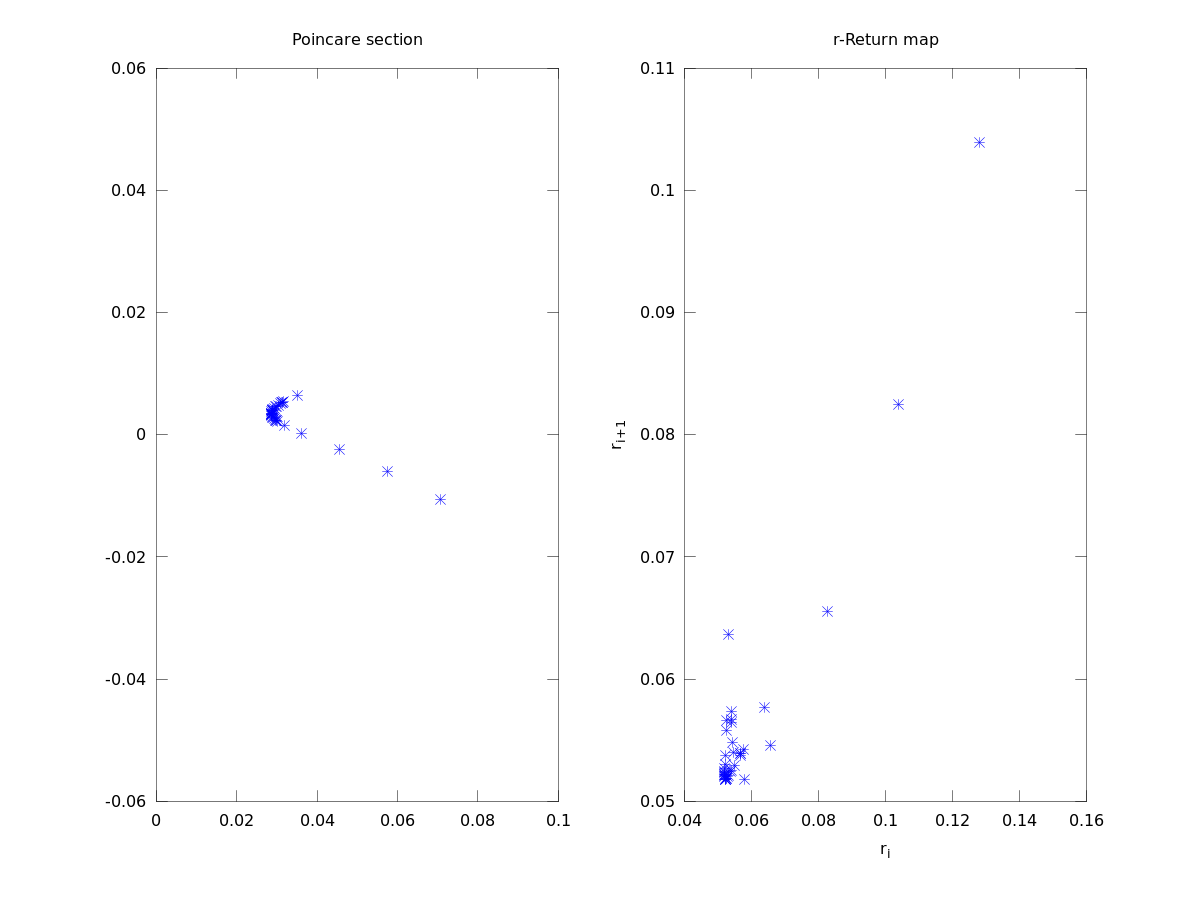
\includegraphics[width=0.9\textwidth]{BBdanielvariedpoincare}
  \end{center}
  \caption{Left: Poincar\'e section for the \twoMode\ flow shown in
  \reffig{fig:BBdanielvariedflow}. Section hyperplane passes
  through $\hat{x} = (u=2.5, v=12, w=0, q=0)$ and the plane normal is
  $\hat{n} = (-12,2.5,0,0)$ ($\hat{x}$ rotated 90 degrees about $w$
  axis). Right: Poincar\'e return map of radial distance from $w$
  axis.}
  \label{fig:BBdanielvariedpoincare}
\end{figure}


\item[2013-08-24 Predrag to Daniel] Looks like this might result in a
publication. At what point do you think we should invite the original
cgang contributors, offer them a chance to join this? In my case, I
believe that a co-authorship should require a substantial
contribution, minor ones go into the acknowledgments.

\item[2013-08-25 Daniel to Predrag] Well, I think only Keith expressed interest originally. Anyway, I think if we are going to get them involved with this, it might as well be sooner rather than later so that they can make a significant contribution (and don't have too much to catch up on, which might disincentivize them to actually do anything).

\item[2013-08-25 Predrag] Can you contact him? If you search through
the blog, Bryce seems to have contributed, even though he was MIA
when we wrote the `atlas' article; maybe someone else too who we have
forgotten by now. Tell them both that they can be coauthors if they
contribute to the research content AND actively write and edit the
article.

\item[2013-08-31-2013 Daniel to C-gang] Contacted Keith, Bryce, and Lei (I'm assuming Siminos is already in the loop). Only heard back from Bryce, who said he is interested. Told him to coordinate with Burak since they are both taking Predrag's QFT class.

\item[2013-08-24 Predrag]
The general drift if where you are going looks promising. Remember,
you always must check whether the single slice hyperplane reduced
dynamics crosses the chart border. If it does, pick a 2. template
(that captures dynamics that lies beyond), and check that dynamics
crosses the two-slice hyper-planes ridge before it hits the chart
border. And so on. Looking forward to drawing the 3-slabs drawing for
the 3 slices case.

To make sure you understand this (Daniel does), email now appointment
time to Ashley ashleypwillis@gmail.com and Kimberley for Monday, and
explain to them how this works. It is very important to do it as soon as
possible, as Ashley is trying to implement it for pipes right now and
does not understand it (nobody reads papers\rf{atlas12} nowadays -
the situation is hopeless :) (but good). And he is here only for 10
days more.

You might also get Kimberly into this git. So far she has not learned
to use svn either :)

\item[2013-08-25 Burak] I am sending Kimb the invitation to the Google updates group and the quick start guide (for Debian-based Linux Distros. I am also blogging it in \texttt{strategy.tex}) you can give her collaborator access once she gets herself a gitHub account.

\item[2013-08-25 Burak] Using the parameters in
\refeq{eq:PKDanielParsVaried},
%([2013-09-02 Burak]
except that in this numerical search, I
mistakenly used $b_2 = -0.00144$ (see [2013-09-02 Burak] for the
discussion), I scanned the invariant coordinates $u$
and $v$ from 0 to 1000 (increasing each by steps of 10) and looked
for a \eqv\ starting a Newton-Raphson search from each $(u,v)$
combination. Code is here:
\\
\texttt{/blog/burak/PorterKnobloch/rootfinding/pkroots.m}. The \eqva\
that I found are
\bea
(u,v,w,q) &=& (0,0,0,0)
    \continue
		  &=& (0.12496, 0.62510, -0.18504, -0.06933)
	\continue
		  &=& (0.21517, 373.61171, -8.31743, -0.11355)
	\continue
		  &=& (0.02618, 373.61171, -1.01417, -0.01386)
	\continue
		  &=& (0.13684, 374.34003, -5.29472, -0.07231)
	\continue
		  &=& (0.00269, 375.58562, -0.10412, -0.00142)
	\continue
		  &=& (0.37194, 372.15177, -14.34919, -0.19577)
	\continue
		   &=&     (0,425.56,0,0)
\,.
\label{eq:PKDanielParsVariedEqva}
\eea
(for the last one, see {\bf [2013-08-26 Burak]} below)

\item[2013-08-25 Predrag] Wow!

\item[2013-08-25 Burak]
Corresponding stability matrix eigenvalues in respective order:
\bea % DB resorted eigenvalues by decreasing real parts 8/30/2013
\lambda_i &=& (1.22560,-4.99180 \pm 2.17690i,-5.60460)
    \continue
		   &=& (0.02993 \pm 1.97539i, -5.82124, -11.62009)
	\continue
		   &=& (7.99278, -10.73945, -159.45337, -318.12740,)
	\continue
		   &=& (2.74751,-3.87388,-159.32547, -318.65092)
	\continue
		   &=& (6.44915,-8.52430,-159.40058, -318.34481)
	\continue
		   &=& (0.69456,-1.61956,-159.30945, -318.71575)
	\continue
		   &=& (10.22285,-14.31342,-159.55807, -317.69045)
\,.
\label{eq:PKDanielParsVariedEqvaEvals}
\eea
Each found \eqv\ has at least one positive eigenvalue.

\item[2013-08-25 Predrag]
I find it easier to survey $\{\Lyap_j\}$ if one lists them by
decreasing real parts
$\eigExp[j] = \eigRe[j] \pm i\,\eigIm[j]$. The most worrisome is
$0.02993 \pm i\,1.97539$; why is it so close to being marginal?
 You also need the
eigenvectors $\jEigvec[j]$ to make sense of how these fit together.
You use the unstable ones to start tracing (short) segments of
unstable manifolds, to see where they go; some examples are in
\refref{SCD07} and \wwwcb{/tutorials}.

\item[2013-08-25 Burak] I also computed the dynamics within the reduced space and generated the exact same trajectory that I got from the direct integration in the full \statesp\ using the parameters in \refeq{eq:PKDanielParsVaried}. You can reproduce this result by following the directions in [2013-08-23 Burak].

\item[2013-08-25 Daniel] Hmmm... according to our results from ca. 2012-04-28 which are around \refeq{PKinvEqs5a} in the manuscript, we should have 8 \eqva: the origin, $(0,-\mu_2/b_2,0,0)$, and six others that we haven't been able to solve for analytically at the time. Did no $(0,-\mu_2/b_2,0,0)$ \eqv\ pops out this time? I think that HAS to be there, independent of parameters. Just in case, I checked all the \eqva\ listed by Burak in \refeq{eq:PKDanielParsVariedEqva} and they all seem to satisfy the syzygy \refeq{eq:syzPK} (at least to a couple of decimal places since Burak only listed the values are only listed to 5 decimal places).

\item[2013-08-26 Burak] I checked and confirmed that $(0,-\mu_2/b_2 = 425.56,0,0)$ is indeed an \eqv\ and it is stable. I also started simulations from the each \eqva\ I posted above at
\refeq{eq:PKDanielParsVariedEqva} they all ended up going towards the strange attractor. I think I'll be able to get $(0,-\mu_2/b_2,0,0)$ also hyperbolic or unstable, now that we have an analytic expression for where the root is, it will be fairly straightforward.

\item[2013-08-26 Daniel to Burak] Remember that $u$ and $v$ are constrained to be positive since they are $x_1^2+x_2^2$ and $y_1^2+y_2^2$ in disguise. I might be possible to just restrict $-\mu_2/b_2$ to be a negative number so the equilibrium is in a part of phase space that we don't care about.

\item[2013-08-30 Daniel] After discussing with Predrag, I tried playing around with the parameters a little bit to see if I could get rid of some of them and still maintain chaotic dynamics. I discovered that it is possible to get reduce the number of parameters to 4 (or maybe 5, no sure if setting $e_2 = 1$, counts as removing a parameter) by basically either zeroing out parameters or setting to 1 or -1. Here's a set that gives some nice chaos:
\bea
\mu_1&=&-2.8023, \mu_2=1, a_1=-1, a_2=-2.6636
    \continue
b_1  &=& 0, b_2=0, c_1=-4.1122, c_2=1.8854, e_2=1
\,.
\label{eq:PKDanielParamsReduced}
\eea
The attractor looks pretty much the same as what we have been seeing with the parameter sets from \refeq{eq:PKDanielParsVaried} and \refeq{eq:PKChaoticParams}. Notice that two terms are wiped out completely ($b_1$ and $b_2$ are zeroed out so it simplifies things a little bit.
Furthermore, I think it sends the extra attractor $(0,-\mu_2/b_2,0,0)$ out to infinity, so the strange attractor might be the only one. Burak, maybe you can run your root finder with this set of parameters and see what happens to the other roots?

The Lyapunov exponent calculation using these parameters gives
\beq
\{\lambda_i\} = \{0.117,\, 0.00, \,-5.7,\,-11.2\}
\,,
\ee{eq:PKLyapunovExp1}
to be contrasted with $$ \{0.09,\, 0.00,\, -9.14,\,-17.77\}
$$ from \refeq{eq:PKLyapunovExp}.

As Predrag has stressed earlier this probably isn't the optimal thing
to calculate, but at least tells us that there is a positive Lyapunov
exponent.

\item[2013-08-30 Burak]
I searched for roots using Daniel's new simplified set of parameters starting
from different initial guesses as I did for the previous case. I only found
$(0.19346,0.54822,-0.28187,-0.05119)$ other than the origin with the stability
matrix eigenvalues $(-11.01364, 0.05064 \pm i 2.45364, -5.51033)$. I also
simulated the system with these parameters and calculated the Poincar\'e
section and I confirm chaotic behavior.

    \PCedit{
\item[2013-08-31 Predrag]
What is striking about the \eqva\ in
\refeq{eq:PKDanielParsVariedEqva} are the $v \approx 375$ values,
while the attractor $v$ values are of order 10. These \eqva\ are
unlikely to play any significant role in shaping the strange
attractor. Can you find values of parameters that send these off to
infinity? If so, can That might reduce the order of the polynomial, and perhaps
reduce the number of parameters to a few?

The logic of the paper would then be:
\begin{itemize}
\item We would like to illustrate how the interplay of different
  physical modes complicates group orbits, and necessitates slicing
  by a set of chart.
\item $N=2$ truncation of \KS\ is too radical to exhibit any
  interesting dynamics, so we adopt the well studied $\SOn{2}$
  symmetric bifurcation normal form {\twoMode} system as our starting
  model. Unfortunately it has 7 parameters, none with physical interpretation
  when dynamics is far from the bifurcation.
\item However, we note that most \eqva\ tend to lie very far from the
  strange attractor of interest. We chose parameters such that these
  \eqva\ are sent off to infinity, thus reducing the number of
  parameters to ??. Some of these we can set to simple values without
  losing the qualitative dynamics of interest, and thus our model is
  ??-parameter sub-model of the {\twoMode} model.

\end{itemize}
    }

\item[2013-08-31 Daniel to Burak] For some reason, I haven't been able to get your rootfinding code to work. It must be some Matlab/Octave translation thing and I'm not really sure how it works anyway. As Predrag discussed above, it would be nice to have an excuse for setting some of the parameters to zero, for example, that doing so sends some of the roots off to infinity. I have a theory that the magnitude of the solutions that you found for your modified set of parameters is large because they go like 1/a small parameter. The only small parameters in your parameter set are $b_1$ and $b_2$. Setting $b_2$ to zero sends $(0,-\mu_2/b_2,0,0)$ to infinity, so might be possible that $b_1$ controls the other ones. Could you start from \refeq{eq:PKDanielParsVaried}, set $b_2$ to zero, check if this affects the roots. If not, make $b_1$ a little bit smaller and see if they move further away from the origin. If they do, make it even smaller and see if they go further out. This might be a way to justify zeroing out $b_1$.

\item[2013-09-02 Burak] To have a better understanding of the behavior of the fixed points, I started from \refeq{PKinvEqs5b}, scaled variables and parameters back to the ones without tilda, and solved $f(u,v) = 0$ for $u$. Since this polynomial is of degree 2, I got two possible solutions for u:
\bea
u_{root,^1_2}(v) &=& -\frac{B}{2A} \mp \frac{\sqrt{\Delta}}{2A}
\continue
&& \mbox{where } \Delta = B^2 - 4AC ,\, A = a_1 c_2 ,\, B = -v a_2 c_1 + v b_1 c_2 + c_2 \mu_1 ,\,
\continue
&& \qquad \quad C = -v^2 b_2 c_1 - v c_1 \mu_2 .
\label{eq:uroot}
\eea
Since $v$ and $u$ are always greater than 0, only positive root in \refeq{eq:uroot} has a meaning for the \twoMode\ system, however, which one is positive depends on the parameters and the value of $v$. I substituted these roots into the unscaled $g(u,v)$ from \refeq{PKinvEqs5b} and got the following equations for $v$
\begin{subequations}\label{eq:F1F2}
\begin{align}
 F_1(v) &= g(u_{root,1}(v), v) = 0
\\
 F_2(v) &= g(u_{root,2}(v), v) = 0
\,
\end{align}
\end{subequations}
Now, we have two polynomials of one variable roots of which are the roots of \refeq{PKinvEqs5b}.
By looking at the behavior of these polynomials, I realized a few things. First: There was a typo in my numerical calculation of the fixed points for the parameters given by \refeq{eq:PKDanielParsVaried}. In the numerical calculation, I entered $b_2 = -0.00144$ instead of $-0.0144$ and this resulted in finding a fixed point around $v = 375.368$ with a positive corresponding $u = 0.0261764$. If I had done that calculation correctly with parameters \refeq{eq:PKDanielParsVaried}, I wouldn't find any of the roots with $v = 375.368$, because with the correct value of $b_2 = -0.0144$, this root of $F_1(v)=0$ is shifted to the $v=392.35$ where the corresponding $u$ is $u=-1.82583$ and since a negative $u$ value is not allowed, the fixed point disappears.
This method of looking for the fixed points confirmed my previous numerical foundings. For the parameters given by \refeq{eq:PKDanielParamsReduced} variation of $F_1(v)$ with $v$ is shown in \reffig{fig:BBF1vpars88}.
\SFIG{BBF1vpars88}{}{
	Variation of $F_1(v)$ given by \refeq{eq:F1F2} evaluated with the parameters \refeq{eq:PKDanielParamsReduced}. Note that the curve intersects the $v$ axis at $v = 0.548221$ which is the only fixed point of this system other than the origin. Numerical evaluation shows that this curve monotonically decreases, hence there is no other fixed point.
}{fig:BBF1vpars88}
I am committing the Mathematica file that I used to compute these polynomials at \texttt{/blog/burak/PorterKnobloch/Mathematica/PKfggeneral.nb}.

%\newpage
\item[2013-09-05 Burak]
I tried to develop a way of finding two templates that can capture the dynamics completely and failed. Here is the explanation of what I did:
For a chosen template point $\slicep$, \chartBord\ $\sspRSing$ is defined by the following equations:
\bea
	\braket{\sspRSing}{\sliceTan{}} &=& 0 ,
	\continue
	\braket{\groupTan(\sspRSing)}{\sliceTan{}} &=& 0 .
	\label{eq:chartBord}
\eea
By solving these equations symbolically, we can write the \chartBord\, $\sspRSing$, as a vector of two independent components and two components that are uniquely determined by the independent ones consistent with the fact that the \chartBord\ defines a $(d-2)$ dimensional manifold. The result is
\\(see \texttt{/blog/burak/PorterKnobloch/Mathematica/PKchartborder.nb}
for the computation):
\bea
	\sspRSing &=& \left\{\sspRSing_1, \sspRSing_2,
     \frac{-\sspRSing_1 (\slicep_1 \slicep_3 + 2 \slicep_2 \slicep_4) -\sspRSing_2 (\slicep_2 \slicep_3 - 2 \slicep_1 \slicep_4)}{ 4(\slicep{}_3^{2} + \slicep{}_4^{2} )},
                  \right.
\ceq
                  \left.
     \frac{-\sspRSing_1 (-2\slicep_2 \slicep_3 + \slicep_1 \slicep_4) - \sspRSing_2 (2 \slicep_1 \slicep_3 + \slicep_2 \slicep_4)}{4(\slicep{}_3^{2} + \slicep{}_4^{2} )}
                  \right\}
\,.
	\label{eq:chartBordSol}
\eea
After having an expression for the \chartBord, I tried to come up with a condition of a good choice of two templates $\slicep_1$ and $\slicep_2$. According to my argument (I'm not 100\% sure that this is correct, please check. I suspect that it is too restrictive.), if the following inequalities are satisfied, $\slicep_1$ and $\slicep_2$ provide a two chart atlas that can capture dynamics avoiding the chart borders:
\begin{subequations}\label{eq:F1F2}
\begin{align}
	\braket{\slicep{}^{(1)}-\slicep{}^{(2)}}{ \sliceTan{}{}^{(2)}} \braket{\sspRSing{}^{(1)} - \slicep{}^{(2)}}{ \sliceTan{}{}^{(2)}}  &< 0
	\label{eq:goodtempineqsa}
\\
	\braket{\slicep{}^{(2)}-\slicep{}^{(1)}}{ \sliceTan{}{}^{(1)}} \braket{\sspRSing{}^{(2)} - \slicep{}^{(1)}}{ \sliceTan{}{}^{(1)}}  &< 0
	\label{eq:goodtempineqsb}
\,
\end{align}
\end{subequations}
I tried to sketch how I got these inequalities on \reffig{fig:BB2charts}. Difference vectors shown in red color are the ones which are dotted with the template tangent in \refeq{eq:goodtempineqsa}. My claim here is that the dot products of these vectors, ($\slicep{}^{(1)}-\slicep{}^{(2)}$) and ($\sspRSing{}^{(1)} - \slicep{}^{(2)}$), with the template tangent $\sliceTan{}{}^{(2)}$ should have opposite signs if they are on the different sides of the ridge. \refeq{eq:goodtempineqsb} is the same condition for the first chart.
\begin{figure}
\begin{center}
  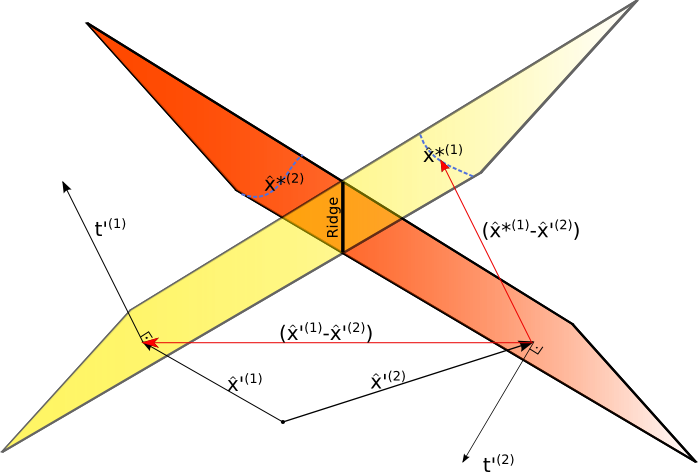
\includegraphics[width=0.8\textwidth,clip=true]{BB2charts}
\end{center}
  \caption{Sketch of a ``good'' two-chart atlas where the respective borders of both charts are on the side of the ridge that the templates are not.}
\label{fig:BB2charts}
\end{figure}
After getting equations \refeq{eq:chartBordSol}, \refeq{eq:goodtempineqsa} and \refeq{eq:goodtempineqsb}, I numerically picked a first template point $\slicep{}^{(1)}$ on the \reqv\ of the \twoMode\ system with parameters \refeq{eq:PKDanielParamsReduced}, then applied group transformation on this point and picked the result as a second template candidate (I thought this would be a good start since this way it is possible to transform the normal vector in a systematic manner, as a function of $\phi$, rather than pulling a random candidate):
\beq
	\slicep{}^{(2)} = \LieEl (\phi) \slicep{}^{(1)}.
	\label{eq:slicepcandidate}
\eeq
With the candidate template \refeq{eq:slicepcandidate}, I evaluated \refeq{eq:goodtempineqsa} and \refeq{eq:goodtempineqsb} and checked their signs. I assigned a range of parameters to the free parameters in \refeq{eq:chartBordSol} and evaluated \refeq{eq:goodtempineqsa} and \refeq{eq:goodtempineqsb} at each combination. If algorithm finds that at least one the inequalities are not satisfied, it varies group operation parameter and repeats the process. My intention was to keep the second template point for which the inequalities were simultaneously satisfied, however, this never happened. Then, instead of picking second template by transforming first one, I started generating random candidates and checked if the inequalities satisfied, again did not get anything worked.

Questions to everybody: Does the reasoning behind equations \refeq{eq:goodtempineqsa} and \refeq{eq:goodtempineqsb} make sense to you? Do you see anything too restrictive in the procedure I described?

\item[2013-09-14 Burak] I computed \twoMode\ dynamics with Daniel's simplified parameters \refeq{eq:PKDanielParamsReduced} for a long time interval,
$t = (0,1000)$, starting close to the \reqv.
\PCedit{{\bf [2013-09-14 Predrag]} Which one?} I reduced it onto one slice defined by the template $\slicep = (1,1,0,0)$ using moving frames. I also computed the dynamics directly starting on the slice hyperplane; plots of both are on \reffig{fig:BBSingleSliceReducedDynamics}. As you can see, they are not exactly the same, \reffig{fig:BBSingleSliceDifference} shows when they start to be different and how different they are.

\begin{figure}%[ht]
  \begin{center}
  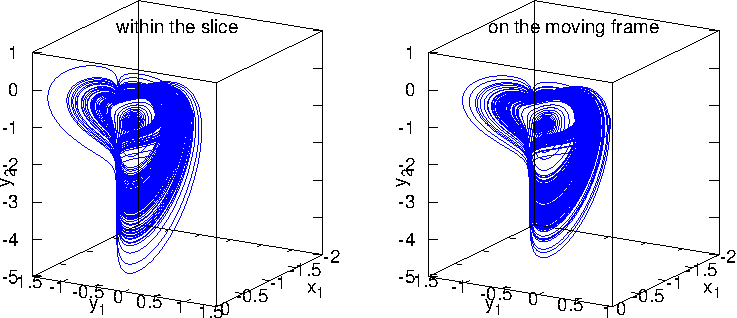
\includegraphics[width=0.9\textwidth]{BBSingleSliceReducedDynamics}
  \end{center}
  \caption{Left: Dynamics of \twoMode\ system with the parameter set
  \refeq{eq:PKDanielParamsReduced}
  integrated
  \PCedit{
  within the $3D$ \slicePlane\ normal to the group tangent $\sliceTan{} =
  (1,-1,0,0)$. The 2D \sliceBord\ plane is in these coordinates the
  $\{0,y_1,y_2\}$ plane normal to the 4-vector $(1,1,0,0)$. As the
  \sliceBord\ coincides with the $m=2$ flow-invariant subspace, the
  symmetry-reduced flow cannot cross the \sliceBord.
  }
  Right: Symmetry reduced dynamics of \twoMode\ system with the parameter
  set \refeq{eq:PKDanielParamsReduced} computed using Moving Frames
  Method.}
  \label{fig:BBSingleSliceReducedDynamics}
\end{figure}

\item[2013-09-14 Predrag] Are the coordinates of
\reffig{fig:BBSingleSliceReducedDynamics} the coordinates of the
\slicePlane, \ie, are they Gram-Schmidt orthogonal to the \template\
group tangent $\sliceTan{} = \Lg\slicep = \Lg(1,1,0,0)= (1,-1,0,0)$ ?
Plot all \reqva; their unstable manifolds might be giving the shape
to your strange attractor. Can
you also draw the 2D \sliceBord\ plane in these coordinates, so one can
see that this \slice\ is a half of a 3D hyperplane? You probably want to
rotate your 3D Matlab projection, so the \sliceBord\ is the back wall,
not the front one. As it contains the
pure $m = 2$ Fourier mode flow-invariant subspace, the \reqv\ in this
subspace might be important in shaping the dynamics.

\item[2013-09-14 Burak]
As you can see from \reffig{fig:BBSingleSliceDifference}, full \ssp\
trajectory computed by two methods are same (to the machine precision)
for the first 200 time steps and then they start to differ around t=250.
If we look at the point on the trajectory for this time, we see that the
trajectory passes through the region given by $x_{1,2} \approx 10^{-5}$
which is quite close to the chart border $x_{1,2} = 0$ as a result, reduced
state space evolution equations comes close to the divergence (but does
not diverge) and starts to generate numerical errors. I used the same fixed
timestep for both calculations and this result shows that this is not a
good idea. One needs to use an adaptive time-stepping algorithm, that would
ensure a certain precision, especially for the flow within the slice. I'm
99\% sure that single slice will work for \twoMode\ system after integrating
a little bit more care.

The reason that I'm sure that single slice would work for \twoMode\ system
has to do with its invariant subspace. In the invariant polynomial basis,
the invariant subspace is $(u,v,w,q) = (0,v,0,0)$ which corresponds to
$(x_1,x_2,y_1,y_2) = (0,0,y_1,y_2)$
in the full state space which is the \chartBord. Hence the dynamics that
would start outside the \chartBord\ will never get into the \chartBord\
in the \twoMode\ system. In other words, in \twoMode\ system, the invariant
subspace is the subspace where the dynamics is confined into the pure $m=2$
Fourier mode. Since the \twoMode\ system is the most general system with
2 Fourier modes, this urges me to check whether a similar statement can
be made in systems with higher Fourier modes. Namely, if we can show that
all invariant subspaces of an m-mode \SOn{2}\ symmetric system will exclude
$m = 1$ region, we can say that an m-mode \SOn{2}\ symmetric system can always
be symmetry reduced using a single slice given by $(1,1,0,0,0,...)$ without
any trouble. I'll be working on this for a while before fixing integration
routines which is a rather more trivial task.

\begin{figure}%[ht]
  \begin{center}
  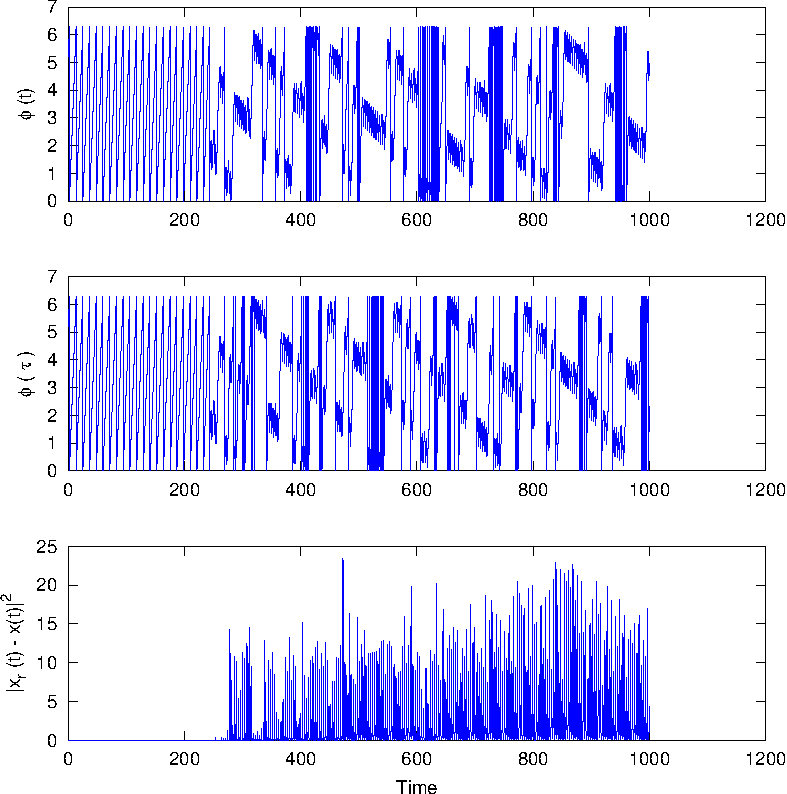
\includegraphics[width=0.9\textwidth]{BBSingleSliceDifference}
  \end{center}
  \caption{
  [Top] Group parameter versus time obtained from the computation of
  dynamics within the slice. [Middle] Group parameter versus time
  obtained from the moving frames calculations. [Bottom] Square of
  the Euclidian norm of the difference between state vectors
  calculated both ways. Parameters are listed in \refeq{eq:PKDanielParamsReduced}.
  }
  \label{fig:BBSingleSliceDifference}
\end{figure}

\item[2013-09-14 Predrag] It's OK, \reffig{fig:BBSingleSliceDifference}
is as it should be. You have probably frequently passed close to $x_{1,2} \approx 10^{-5}$
before $t=250$, doubt that that is the cause of the loss of accuracy;
the trajectory has positive stability exponents.
Flow within the slice is an integration independent
of the moving frame post-processing, with independent computational
errors, so for unstable flow they should agree only up to the Lyapunov
time. \Rpo s are great, because once you start computing them, they should
agree to whatever accuracy you want to compute them, an so will their
Floquet multipliers.


\item[2013-09-14 Predrag] A very minor gripe: your edits are all line per
paragraph. It's OK in wrapping mode in editors, but it is impossible to
read on GitHub.com site, because they are shown as single lines,
extending forever off the screen. If your editor can format paragraphs,
maybe use that? If it is inconvenient, ignore this, it does not matter.


\item[2013-09-18 Daniel] So I guess I'm a little late to the party but
I adapted my old code for slicing \cLf\ to slice the \twoMode\ system in Cartesian
$(x_1, x_2, y_1, y_2)$ coordinates using
$(1, 1, 0, 0)$ as a template and basically get the same result as Burak did
2013-09-14. I can confirm that the trajectory never appears to cross a chart
boundary (i.e., $\dot{\phi}$ stays bounded and never appears to blow up).
I also plotted the results projected onto a Gramm-Schmitt basis orthogonal to the group
tangent $(1, -1, 0, 0)$ such that $v_1 = (\sqrt(2)/2, \sqrt(2)/2, 0, 0),\,
v_2 = (0, 0, 1, 0),\, \mathrm{and}\, v_3 = (0,0,0,1)$. This does not seem to
make the picture significantly different than what Burak got, so I won't repost
figure in the blog. I have saved rotate-able
Matlab figs in /cgang/Daniel/Matlab/Slicing/SingleSlice(1-1-0-0).fig
and /cgang/Daniel/Matlab/Slicing/SingleSliceInSliceCoordinates.fig if anybody wants
to take a look. The chart border basically sits on the $x_1$ or $v_1$ = 0. planes I've included
the equilibrium at the origin as red dot, but still need to put in the other equilibrium
that Burak found numerically. Burak, could you provide this in $(x_1, x_2, y_1, y_2)$ coordinates?
My bet is that it sits in the middle of the lobe that doesn't have the origin in it...

\item[2013-09-19 Daniel] Ok... so I added Burak's numerical equilibrium from 2013-09-02 to the figures.
To do this, I started with Burak's $v = 0.548221$, plugged into \ref{eq:uroot} to find the root where $u > 0$
and got $u = 0.1934602$. I then converted this to Cartesian coordinates $(x_1, x_2, y_1, y_2) = (\sqrt{u}, 0, \sqrt{v},0)$
and rotated this into the slice. I plotted these as black dots in my Matlab figs (file locations in my post
from 2013-09-18). These points seems to be outside the attractor. I also tried
$(x_1, x_2, y_1, y_2) = (0, \sqrt{u}, \sqrt{v},0)$ and rotated THAT into the slice.
These are plotted in the Matlab figs as magenta points. This actually seemed to work better in the sense that
it plops an equilibrium right down in the middle of the lobed structure, which looks more correct to me. I am kind of
confused as to why I get two different points depending on which point I choose. I guess it has to do with fixing the
relative phase of the two modes? Or maybe my postprocess rotation into the slice code is buggy. Burak, could you check
to see if your code gives different points for the two choices of $(x_1, x_2, y_1, y_2)$?

\item[2013-09-19 Burak] I don't think finding $u$ and $v$ for the roots is enough for mapping it
correctly to the full state space, you have to find $w$ and $q$ as well and then find a
numerical solution to \refeq{eq:PKinvxirels}. My starting point for simulations is one of these
points $(x_1, x_2, y_1, y_2) =  (0.12712, -0.42107, 0.68001, 0,29294)$ corresponding to the equilibrium
in the invariant polynomial basis $(u,v,w,q) = (0.19346, 0.54822, −0.28187, −0.05119)$ (this is the
equilibrium in the invariant polynomial basis that I reported in [2013-08-30 Burak]). Trajectory, for a
while, traces the group orbit of this point until it goes away from it and becomes chaotic.
In my simulations, If you look at the time interval during which the trajectory is on the \reqv\, in the
reduced space, you see that all these points on the group orbit are mapped onto a single point.
As the system evolves in time, trajectory spirals out from this point and this region corresponds to the
small spiral in the center of the attractor in \reffig{fig:BBSingleSliceReducedDynamics}. I coded stuff
using which I can plot these processes separately but my netbook's graphics processors has a problem , so
 I'll be able to blog these hopefully tonight, when I get home.

By the way, I am unable to look at .fig files since I don't have a Matlab installation and I have no way
 of legally getting one since I don't have access to a Georgia Tech computer or money to waste on it. I
 also have endless sympathy for open source things and that's another reason why I don't use Matlab.
 If you can commit your plots as pdf files, without blogging them if you think it's unnecessary, I can
 look at them.

\item[2013-09-19 Predrag] If you need to run Matlab, you can run it on CNS linux network,
or on the MS windows box in the computer cubicle 5th floor Howey W508E.

\item[2013-09-19 Daniel] Fixed figure to include the correct \reqv\,
in the slice projected coordinates. Here's a pdf for poor Burak who
cannot see Matlab figs \reffig{fig:DBSingleSliceReducedDynamics}.
Rotate-able version in /cgang/Daniel/Matlab/Slicing/SingleSliceInSliceCoordinates.fig.

\begin{figure}%[ht]
  \begin{center}
  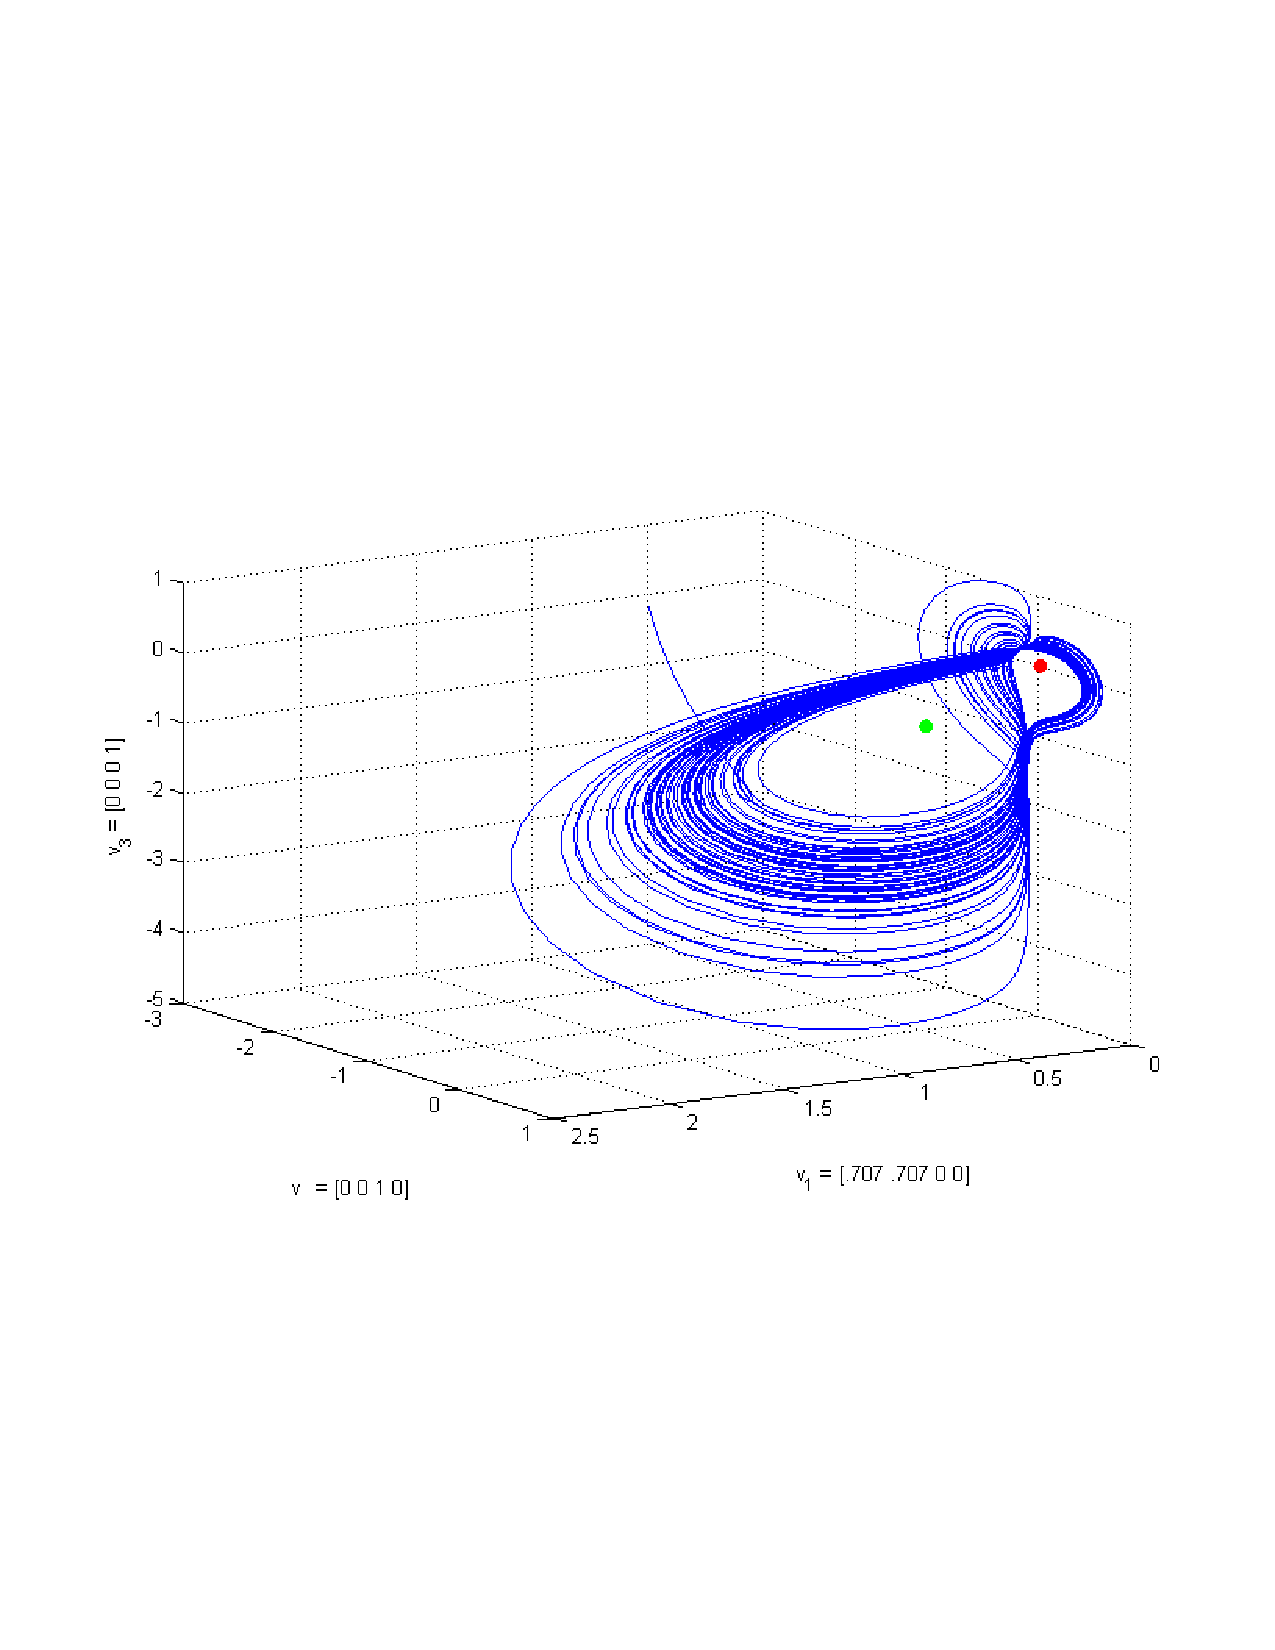
\includegraphics[width=0.46\textwidth]{PKSlicedDynamicsInSliceCoordinates1}
  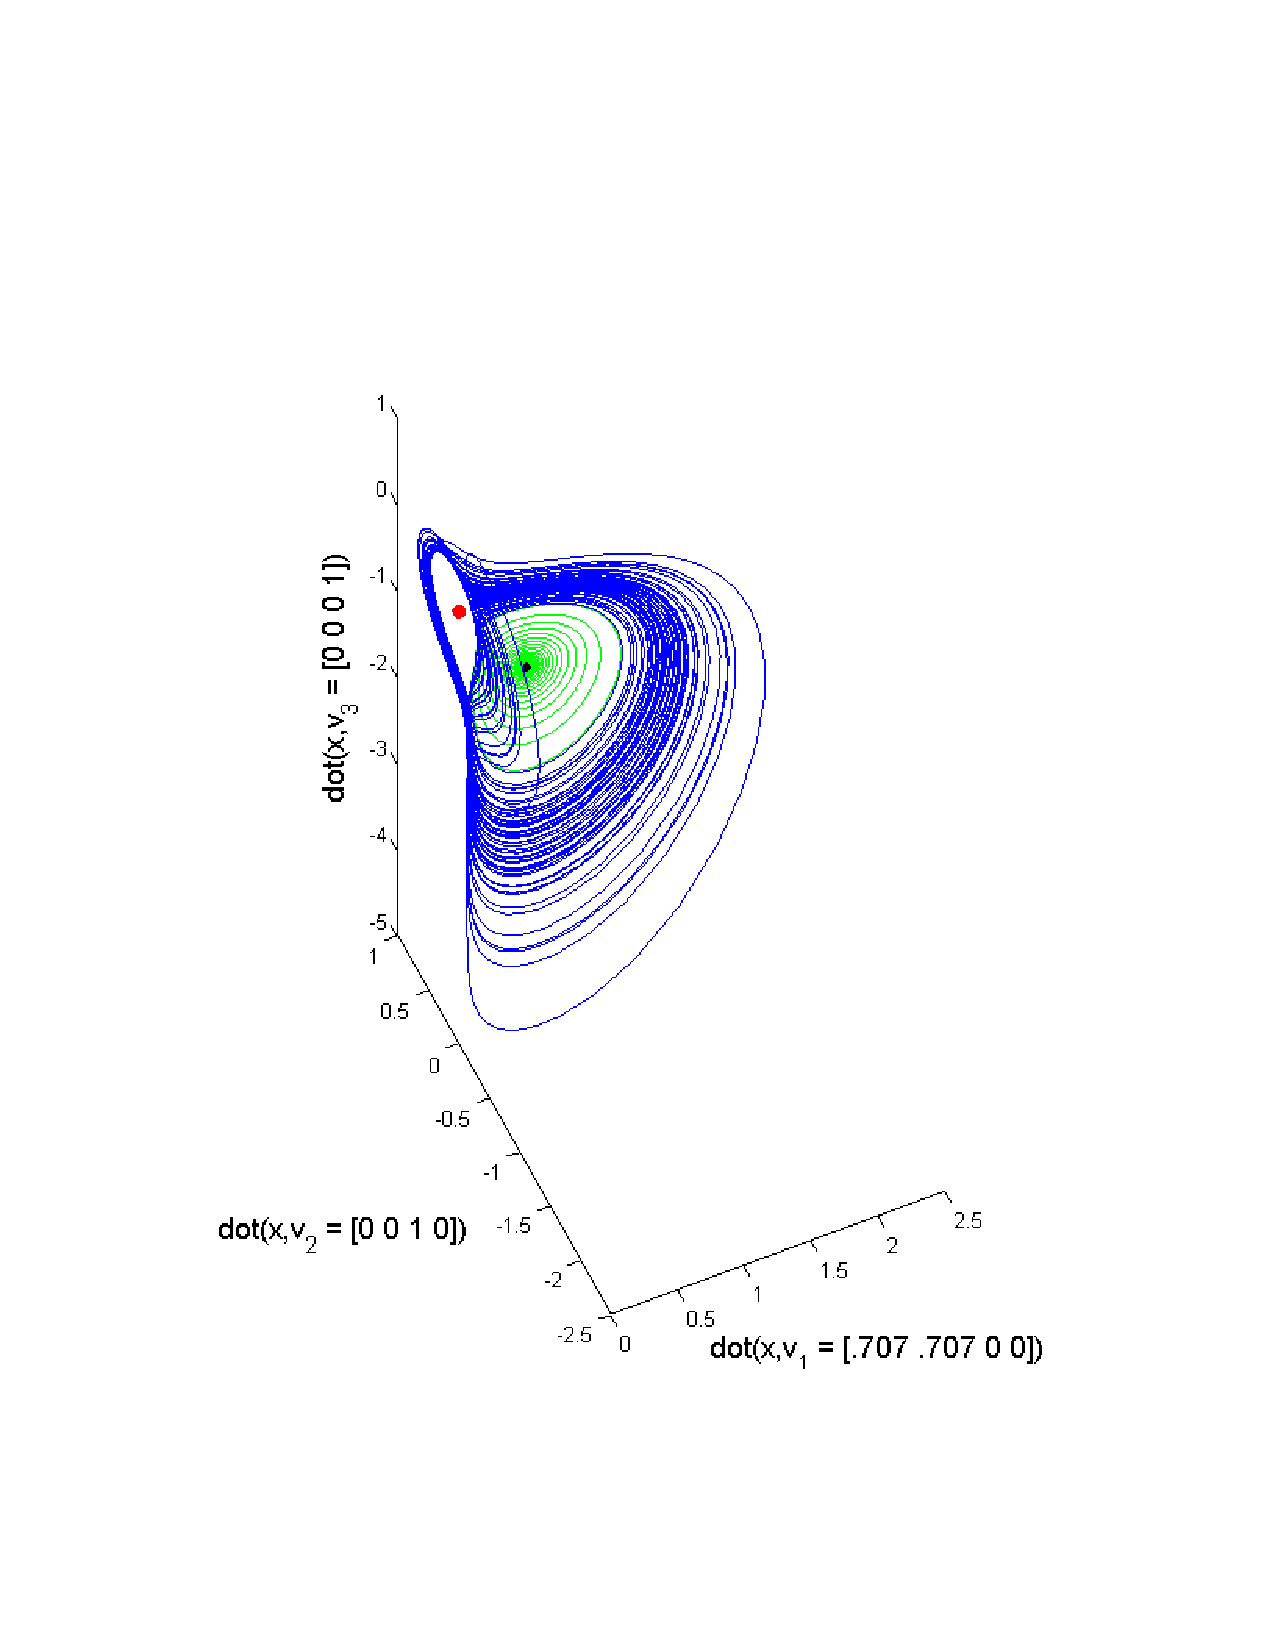
\includegraphics[width=0.46\textwidth]{SingleSliceInSliceCoordinates}
  \end{center}
  \caption{\PCedit{
    Left: The invariant subspace which is also the \slicePlane\ border
    contains the unstable \reqv\ ${}_{NO2?}$ marked red, which shapes the
    `border' part of the strange attractor (EXPLAIN). Right:}
    Dynamics of \twoMode\ system with the parameter set
    \refeq{eq:PKDanielParamsReduced} reduced to a \slicePlane\ of the template
 	$(x_1, x_2, y_1, y_2) =  (1, 1, 0, 0)$ and projected onto a Gramm-Schmitt
 	basis orthogonal to the template group tangent $(x_1, x_2, y_1, y_2) =
 	(1, -1, 0, 0)$. \Reqv\ at the origin is shown in red. Points started near
 	the origin fall into the attractor rather quickly. \Reqv\ ${}_{NO1?}$ is
 	shown in black with a trajectory escaping from it along its unstable manifold
 	and into the attractor shown in green. Once the system leaves this green region
 	it does not come back. Trajectories started away from this region never enter it.
 }
  \label{fig:DBSingleSliceReducedDynamics}
\end{figure}

\item[2013-09-20] Thanks! \reffig{fig:DBSingleSliceReducedDynamics} is very similar to what I got, I'm not
blogging another version of this, I'm moving onto Poincar\'e sections on slice right now, results will hopefully
be here tomorrow.

\item[2013-09-19 Predrag] What about spiralling away from the other \reqv\ ${}_{NO2?}$
in \reffig{fig:DBSingleSliceReducedDynamics}?

\item[2013-09-19 Predrag] This is really looking pretty. Next,
\begin{itemize}
  \item a Poincar\'e section, or more likely two
  \item parametrize it/them using curvilinear length along the
  unstable manifolds of the two \reqva\ - I assume one of them is in
  the invariant subspace?
  \HREF{http://www.streamsound.dk/book1/chaos/chaos.html\#264/z} {See ChaosBook}.
  \item construct return map, forward maps.
  \item describe symbolic dynamics, find a set of \rpo s.
  \item complete the current draft the paper, publish.
\end{itemize}

\item[2013-09-19 Predrag]
Please go to Adam Kamor and learn how to use his
unstable manifold Poincar\'e sections code - looks very smart (Adam
Fox approved), then put a copy of the code into our git  repository
\texttt{/code/}. It should help you get the return maps for the
2-mode problem, and it should become very useful once we symmetry
reduce KS flow (and NS! :)

\item[2013-09-22 Burak]
I started computing Poincar\'e sections on the Gram-Schmidt coordinates.
As a first template, I chose the equilibrium $\hat{x} = (-0.4398, -0.7285, 0.1323)$
(black dot on the middle of the green spiral on \reffig{fig:BBgramschmidt})
and chose the normal vector in such a way that the Poincar\'e section includes
 the vertical axis: $\hat{n} =  (0.85607, -0.51686, 0.00000)$. Points on this
 Poincare\'e section is on \reffig{fig:BBpsectgs}.

\refFig{fig:BBgramschmidt} is equivalent to
\reffig{fig:DBSingleSliceReducedDynamics} 	I am posting this just to
have a reference for the Poincar\'e sections that I am going 	to
present in this blog, since I used my own basis on those.


\item[2013-09-22 Predrag]
I would chose the two \reducedsp\ coordinates
$\{\sspRed_1,\sspRed_2,\sspRed_3\}$ to span the \chartBord/invariant
subspace plane, the 3. one normal to the two (maybe you do that already).
I'm not seeing the Poincar\'e section (Siminos can point you to the
mathematica codes he used to get shading effects), but I would guess
the optimal one would go through the other \reqv\ and cut transversaly
the flow coming closest to the observer; that will probably give you
a very nice return map.

\item[2013-09-22 Burak]
 I then generalized my code for
 arbitrary plane normals (using Euler angles) and observed that the Poincare\'e
 section looks qualitatively same if I rotate the plane around  the vector:
 $(-0.4398, -0.7285, 0)$. I can explain this much better if I can draw these planes
 along with the flow, I tried but could not yet succeeded in this. Do you have a favourite
 software for these kind of plots? (transparent surfaces etc.)

 I'm not sure
 if I can define a useful curvilinear distance using which I can construct the return map.
 To get a better understanding, I will stop coding for a while and read
 the relevant ChaosBook chapters.


\begin{figure}%[ht]
  \begin{center}
  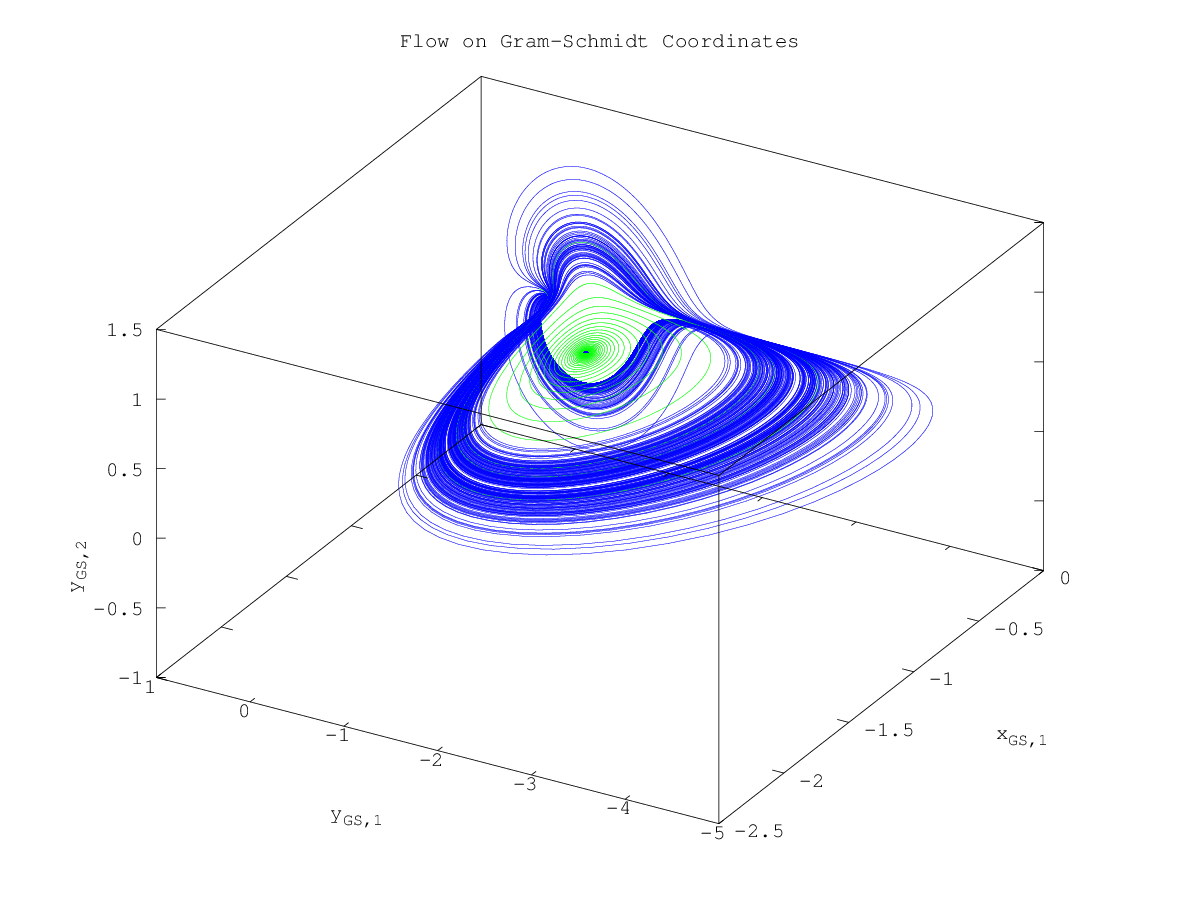
\includegraphics[width=0.8\textwidth]{BBgramschmidt}
  \end{center}
  \caption{
   Symmetry reduced \twoMode\ flow on the Gram-Schmidt coordinates.
 }
  \label{fig:BBgramschmidt}
\end{figure}

\begin{figure}%[ht]
  \begin{center}
  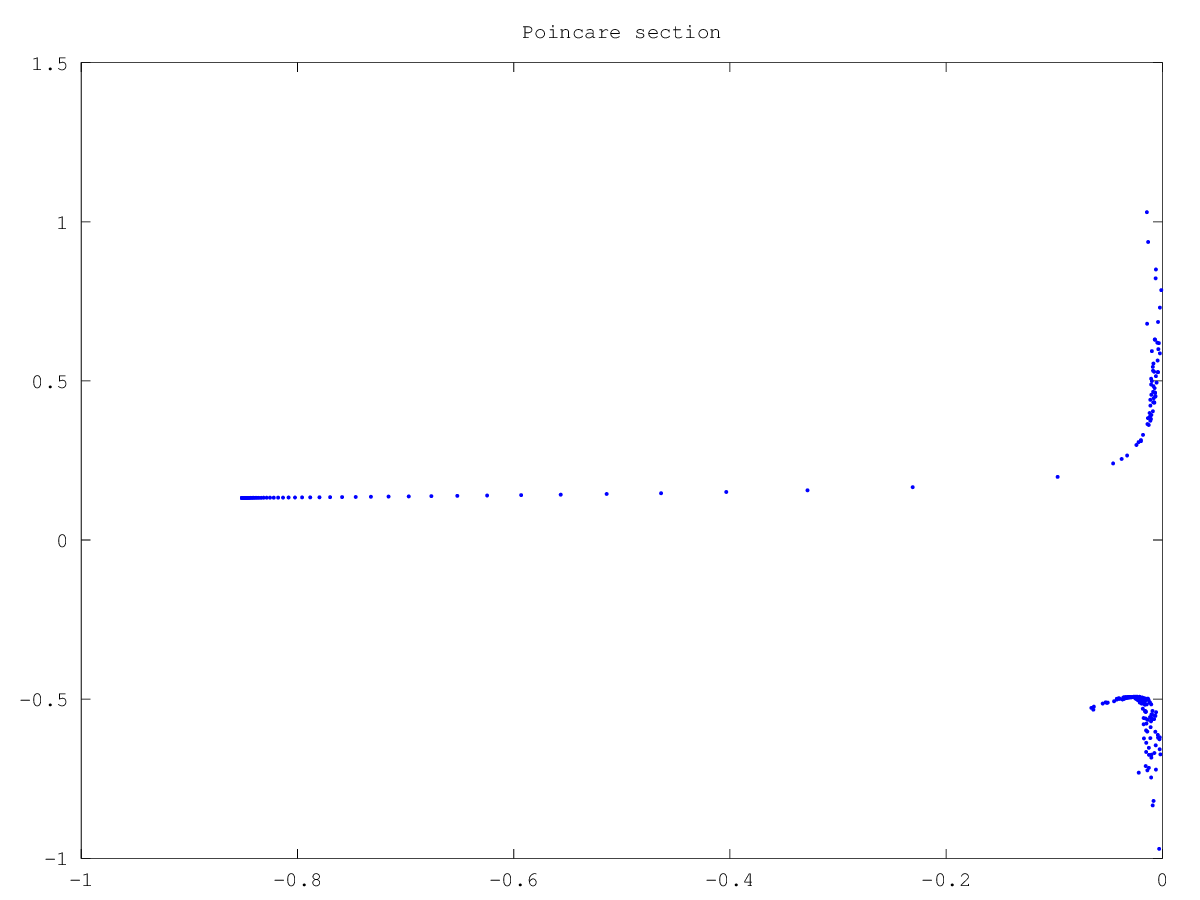
\includegraphics[width=0.8\textwidth]{BBpsectgs}
  \end{center}
  \caption{
	Poincar\'e section plane in the Gram-Schmidt coordinates, defined by
    going through the \reqv\
	$\{\sspRed_1,\sspRed_2,\sspRed_3\} = (-0.4398, -0.7285, 0.1323)$
    and being normal to $\hat{n} =  (0.85607, -0.51686, 0.00000)$.
 }
  \label{fig:BBpsectgs}
\end{figure}

\item[2013-09-22 Predrag] I propose we use the same name for invariant
solutions when plotted in the full $\{x_1,x_2,y_1,y_2\}$ \statesp\ and
the $\{\sspRed_1,\sspRed_2,\sspRed_3\}$ \reducedsp. For example, $\{x_1,x_2,y_1,y_2\} = (0,0,0,0) \to
\{\sspRed_1,\sspRed_2,\sspRed_3\}  = (0,0,0)$ is an \eqv\ (the only one
in this problem, coinciding with the $(0,0,0)$ flow invariant subspace - I
guess every \eqv\ is by definition a 0\dmn\ flow invariant subspace, and
\reqv\ a 1\dmn\ flow invariant subspace). Any full \statesp\ \reqv\ and \rpo\
should still be called that when plotted as \eqv\ and \po\ in the
\reducedsp. Invariant polynomials $(u,v,w,q)$ are only a crutch; except
for the section in which we discuss them, all other \reqv\ and periodic
points should be listed in $\{x_1,x_2,y_1,y_2\}$ and in
$\{\sspRed_1,\sspRed_2,\sspRed_3\}$ coordinates.


\item[2013-09-22 Predrag]
Can you mark the red dot (the unstable invariant subspace \eqv\ at the
origin) in  \reffig{fig:BBgramschmidt}? If I understand you, your single
Poincar\'e section goes through both important \eqva/\reqva\ (if there
are other nearby \reqva, mark them too, the distant ones do not matter).
You might need a pair of Poincar\'e sections, each going through one of
the (\reducedsp) \eqva\ and its stable eigenvector, and than rotated in
some convenient manner, perhaps so it goes through the other \eqv.

\item[2013-09-22 Predrag]
The list \refeq{eq:PKDanielParsVariedEqvaEvals} is missing the stability
eigenvalues for the \reqv\ within the invariant subspace. You also want
to distinguish the eigen-directions which stay within the subspace from
those who go out of it.

\item[2013-09-22 Predrag] to Bryce and Evangelos: It looks like Burak is
doing all the heavy pulling. While Daniel crosschecks the results and
helps him with the final stretch and the figures, can you two complete
the first draft of the article, \refsecttosect{s:intro}{s:concl}, by
October 1, 2013?

\item[2013-09-28 Burak]
Since there are a lot of experimental posts in this blog, I decided to
write a compact summary to clarify which parameter set we are using, what
are the roots and \eqva\ etc. This will help me to have a record
of my own progress and I thought this would also help in writing  the paper.

For the \twoMode\ system defined by \refeq{PKinvEqs1} in invariant polynomial
basis, and \refeq{2mode4D} in 4D \statesp , we use the following set
of parameters, for which the flow is chaotic, suggested by Daniel in [2013-08-30 Daniel]:
\bea
\mu_1&=&-2.8023, \mu_2=1, a_1=-1, a_2=-2.6636
    \continue
b_1  &=& 0, b_2=0, c_1=-4.1122, c_2=1.8854, e_2=1
\,.
\label{eq:PKparamsfinal}
\eea
With these parameters, the system has 2 roots in the invariant polynomial
basis:
\bea
	(u,v,w,q)_{EQ} &=& (0,0,0,0)
    \continue
	(u,v,w,q)_{TW} &=& (0.19346, 0.54822, -0.28187, -0.05119) \,.
\label{eq:PKinvpolrootsfinal}
\eea
I am $(100-\epsilon) \%$ sure that
these are only roots. See [2013-08-25 Burak], [2013-08-30 Burak] and
[2013-09-02 Burak] for the details of finding them. The
bivariate polynomials of \refeq{PKinvEqs5a} simplify significantly with
the choice of parameters \refeq{eq:PKparamsfinal}, and numerical
solutions becomes easier to deal with.

Root at the origin of the invariant polynomial basis corresponds to the only
\eqv\ of the system in the full \statesp, and the second root corresponds
to a \reqv. The details (Jacobians, eigenvalues \& eigenvectors) about these
roots will come soon.

We apply the method of moving frames to reduce the \SOn{2}\ symmetry of the
system using a single template defined by $\slicep = (1,1,0,0)$ for which
the chart border, given by $x_1 = x_2 = 0$, is an invariant
subspace of the \twoMode\ system. Hence, it is safe.
\ES{2013-09-29}{This is true, but at the same time such slices
are of little value for KS and, I think, fluids.
For KS, inclusion of a third mode will break invariance of the $k=1$ subspace
and one would have to worry about crossing it. What would be the
scope of this paper then? What have we really shown? It is a nice study of
the PK system, but can we claim progress in terms of general slicing?}

\BB{2013-09-30}{If you choose your template as, say, $\slicep = (1,0,0,0)$ all
solutions with completely imaginary first Fourier mode will be on the \chartBord .
As you transform this template with the group action for different parameters,
you will get other linear relations between $x_1$ and $x_2$ for the \chartBord .
Only for $\slicep = (x, x, 0 ,0 ,0 ...)$ (see main blog for the proof), \chartBord\
becomes $x_1 = x_2 = 0$.
\BBedit{(FALSCH. SEE \texttt{siminos/blog} [2013-11-18 Burak] FOR CORRECTION.)}
By an ``improper domain'' I mean this: Let's say you have
a square wave with the frequency $\omega_0$, if you Fourier expand this
function with the harmonics of $\omega_0 / 2$, you will get the first Fourier
mode to be 0, and second mode to be non zero.}

In order to visualise the system in 3D, we define\ES{2013-09-29}{I thought that
GS is a standart procedure to orthonormalize a given set of vectors. I don't see
why you can choose to define this basis any way you want. \BBedit{Here I
refer to the (n-1) basis vectors which are all orthogonal to the slice tangent
as Gram-Schmidt basis and describing one way of choosing such coordinates so
that everyone knows exactly what coordinates that I'm talking about. Motivation
of explaining this choice is just because the choice is not unique.}} the Gram-Schmidt basis
as $e_{i,GS} = \LieEl (\pi/4) e_i $, where $e_{x1,GS} = (0.70711, -0.70711, 0 0)$
is parallel to \sliceTan\ hence the reduced flow has no component in that
direction\ES{2013-09-29}{Then why do you want to use it? \BBedit{I am not using it.}}.
Three Gram-Schmidt coordinates generated this way are:
\bea
	e_{x,GS} &=& (0.70711, 0.70711, 0, 0)
	\continue
	e_{y1,GS} &=& (0, 0, 0, -1)
	\continue
	e_{y2,GS} &=& (0, 0, 1, 0)
	\label{eq:GramSchmidtBasis}
\eea
\ES{2013-09-29}{Is it really $e_{x,GS}$ or is it $e_{x1,GS}$? Is there a missing or
extra minus sign? \BBedit{Since the reduced flow has no component in $x_{1,GS}$
direction, I just took $x_{2,GS}$ and dropped the index.}}

Here, the choice of $e_{y1,GS}$ and $e_{y2,GS}$ might seem unnecessary
since it would work if they were kept the way they were before. The reason
I defined them this way is to have a consistent procedure of going from one
basis to another using orthogonal transformations. Namely, whenever I want
another set of basis to project things onto, I apply the same orthogonal
transformations to all cartesian basis in the previous coordinate system,
and use the final transformed vectors as the new basis. For example, when I
need a basis to draw things on a particular Poincar\'e section, I will
apply the SO(3) rotations to the usual cartesian basis in such a way that
transformed $e_x'$ will be parallel to the Poincar\'e section normal,
and use the transformed $e_y'$ and $e_z'$ as the basis for the Poincar\'e
section. This way, I will have a systematic procedure for going back and forth.
\ES{2013-09-29}{I still don't understand your motivation for this. Any vector you can
take it onto the slice in a well defined manner, so I don't see the problem
you are trying to solve with this choice of $e_{y1,GS}$ and $e_{y2,GS}$.}

The symmetry reduced \twoMode\ flow on the Gram-Schmidt coordinates, the \eqv ,
the \reqv\ and their respective unstable directions are shown in \reffig{fig:BBunstablevectors}
(I'm sorry for posting almost the same figure for a third time, but the
reason that I'm doing this is to avoid further ambiguities, I am hoping to
stick with the definitions of today's post.). In the following, I will
explain how I got the unstable directions in the figure (It has some intuitive
steps that I'm not sure if they are correct) starting with the origin.
\begin{figure}%[ht]
  \begin{center}
  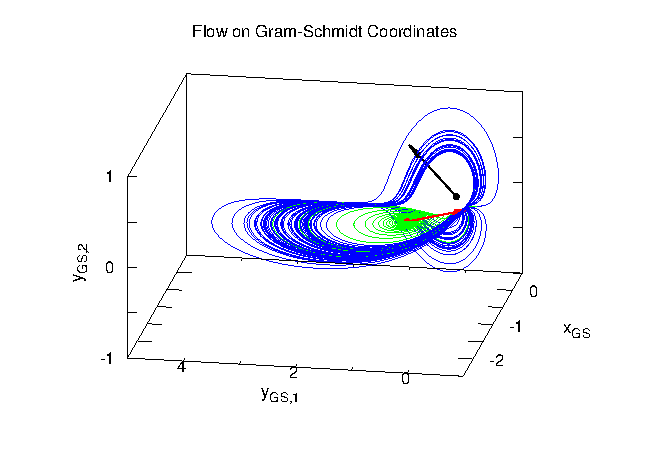
\includegraphics[width=0.9\textwidth]{BBunstablevectors}
  \end{center}
  \caption{
   Symmetry reduced \twoMode\ flow on the Gram-Schmidt coordinates of \refeq{eq:GramSchmidtBasis}
   Initial point of the flow is the \reqv\ of the \twoMode\ system. This
   point and its unstable direction are shown respectively with the red
   dot and the red arrow on the plot. Trajectory spirals out (green) from
   this point and then starts to trace the strange attractor (blue). The
   \eqv\ at the origin and its corresponding unstable direction is shown
   with the black dot and the black arrow.
  }
  \label{fig:BBunstablevectors}
\end{figure}
Stability eigenvalues and eigenvectors (Eigenvalues and eigenvectors of
the matrix $A_{ij} = \partial V_i / \partial x_j$)  of the linearized flow
at the origin of the full \statesp\ are
\bea
	\lambda_1 &=& 1 + 1i , \ v_1 = (0, 0, 0.70711, 0.70711 i)
	\continue
	\lambda_2 &=& 1 - 1i , \ v_2 = (0, 0, 0.70711, -0.70711 i)
	\continue
	\lambda_3 &=& -2.8023, \ v_3 = (1, 0, 0, 0)
	\continue
	\lambda_4 &=& -2.8023, \ v_4 = (0, 1, 0, 0)
	\label{eq:originstability}
\eea
I defined the unstable direction as the sum of the eigenvectors with expanding
eigenvalues (eigenvalues with positive real parts), weighted by exponantials
of their respective eigenvalues (in the ``Jacobians'' language, this corresponds to
multiplying the Jacobian eigenvector with its respective eigenvalue):
\bea
	v_{u,0} &=& e^{\lambda_1}  v_1 + e^{\lambda_2}  v_2
	\continue
		    &=& (0,0,2.07705, -3.23481)
	\label{eq:vuorigin}
\eea
This is the direction towards which a small perturbation near the origin will
expand (\BBedit{right?})\ES{2013-09-29}{Here, you take a direction on the
unstable eigenspace and call it unstable direction.
It is as confusing as it could get, please revise. \BBedit{This is just an
intermediate step to have more guidance while choosing Poincar\'e sections.
I did not know if there was another name for it, or it was completely wrong
to think this way. If it is useless, you can ignore it, if there is a motivation
for a revision, then I can do it.}}.
This vector is already on our \slice\ ($ \braket{\sliceTan{}}{v_{u,0}}=0$).
After projecting onto Gram-Schmidt coordinates and normalizing, I obtained the
black vector of the \reffig{fig:BBunstablevectors}:
\beq
	\hat{v}_{u,0,GS} = (0, 0.84147, 0.54030)
	\label{eq:vuoriginGS}
\eeq
I set up the variational equation for the full \statesp\ to compute the
Jacobian of the \reqv\ . Starting from $\ssp_0 = (-0.3110, -0.3110, -0.1323, -0.7285)$
, I integrated $\dot{\jMps} = \Mvar (\ssp) \jMps, \jMps_0 = \matId$ along
with the system itself for a time $T$, until the trajectory arrives at the
initial point. Eigenvalues ($\Lambda_i$) and eigenvectors ($e_i$) of $\jMps^T$ are:
\bea
	\Lambda_1 &=&  0.99996, \quad		   e_1 = (-0.2013, 0.2013, -0.9432, 0.1714)
	\continue
	\Lambda_2 &=&  0,  \quad			   e_2 = (0.5524, -0.7885, 0.2523, -0,0974)
	\continue
	\Lambda_3 &=&  -1.7910 + 0.1170 i,
	\continue
	 e_3 &=& (-0.0922 - 0.4096i, -0.0567 - 0.4141i,  -0.0794 + 0.0449i, -0.8005)
	\continue
	\Lambda_4 &=&  -1.7911 - 0.1170 i,
	\continue
	e_4 &=& (-0.0922 + 0.4096i, -0.0567 + 0.4141i, -0.0794 - 0.0449i, -0.8005)
	\label{eq:reqvstability}
\eea
\ES{2013-09-29}{There is a discussion on stability of relative equilibria in [2012-07-30 Evangelos]
up to the second comment labeled [2012-08-01 Predrag].
Please try to compute stability of your \reqv\ by considering
it as an equilibrium in reduced space (i.e. do it in a invariant variables) and then
compare with what you get. Also, please try to verify Predrag's suggestion that
you can compute the Floquet multipliers using the eigenvalues on a single point on the
relative equilibrium and the period. \BBedit{What I am doing here is calculating
the Floquet vectors and multipliers along a \reqv\ in the full state space.
If this will be useful in choosing Poincar\'e sections, then I don't see a
motivation for redoing calculations, I will go back to your suggestion if
I cannot manage to get a useful Poincar\'e section.}} Here, the first eigenvalue
is very close to unity and the corresponding eigenvector is in the direction
of the $\groupTan{(\ssp_0)} = \Lg \ssp_0$ which is an expected result, hence
I think I computed the Jacobian correctly. Similar to what I did for the
origin, I calculated the weighted sum of eigenvectors with expanding eigenvalues
to get the unstable direction:
\bea
	v_{u,TW} &=& \Lambda_3  e_3 + \Lambda_4  v_4
	\continue
		    &=& (0.42604,0.30014,0.27399, 2.86727) .
	\label{eq:vureqv}
\eea
I then subtracted the component of this vector in the direction of the group tangent
to isolate its projection at the \slice\ hyperplane (\BBedit{This step intuitively
makes sense to me but I'm not 100\% sure about it}):
\bea
	\hat{v}_{u,TW} &=& v_{u,TW} - \braket{\groupTan{(\ssp_0)}}{v_{u,TW}} \groupTan{(\ssp_0)}
	\continue
		    &=& (0.36309,0.36309,0.27399, 2.86727) .
	\label{eq:vureqvred}
\eea
Finally I projected this vector onto the Gram-Schmidt basis \refeq{eq:GramSchmidtBasis}
and normalized to get
\beq
	\hat{v}_{u,TW,GS} = (0.175506, -0.980014, 0.093648) .
	\label{eq:vureqGS}
\eeq
Eq.~\refeq{eq:vureqGS} is shown with the red arrow on the \reffig{fig:BBunstablevectors}.

Computing Jacobians and drawing vectors took a longer time than I expected
as I had to go back and redo things that before I was sloppy at. I am now
going back to the Poincar\'e sections on which the unstable directions will lie.

\item[2013-09-22 Predrag]
At the moment, nothing substantial to add, only some bookkeeping
suggestions concerning the pretty \reffig{fig:BBunstablevectors}. Once
the figure is almost publication ready -like this one seems to be-
\begin{itemize}
  \item Record in \texttt{reducesymm/figSrc/00ReadMe.txt} the program
that has generated it, perhaps save the program in the appropriate
\texttt{reducesymm/figSrc/...} subdirectory.
  \item If possible, save the figure in TeX or LaTeX format; an example
is \reffig{fig:ReducTraj1}. It looks ugly, but it is a great time
saver in the editing process, as you can insert macros for LaTeX
labels which do tend to change a lot in the article editing process.
  \item Do not include labels like `Flow on Gram-Schmidt Coordinates'.
  \item Trim all white edges around figures like BBunstablevectors.pdf
\end{itemize}


 %% ReducTraj*.* - read dasbuch/book/FigSrc/inkscape/00ReadMe.txt
 \begin{figure}
 \begin{center}
  \setlength{\unitlength}{0.40\textwidth}
  %% \unitlength = units used in the Picture Environment
  \begin{picture}(1,0.8361641)%
    \put(0,0){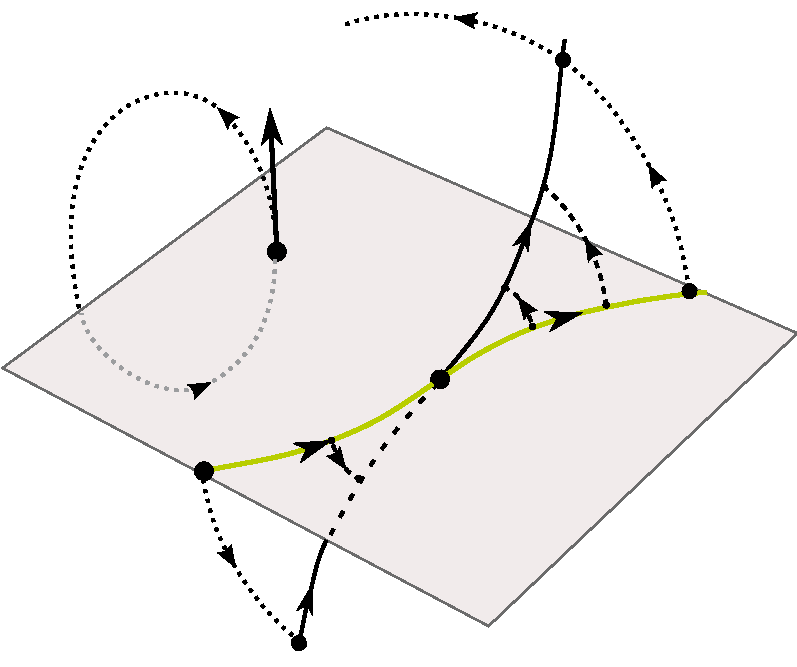
\includegraphics[width=\unitlength]{ReducTraj5.pdf}}%
    \put(0.09054399,0.38282057){\color[rgb]{0,0,0}\rotatebox{-30.34758661}{\makebox(0,0)[lb]{\smash{$\pSRed$}}}}%
    \put(0.57768586,0.29773425){\color[rgb]{0,0,0}\rotatebox{0.0313674}{\makebox(0,0)[lb]{\smash{$\sspRed(0)$}}}}%
    \put(0.59310014,0.69932675){\color[rgb]{0,0,0}\rotatebox{0.03136739}{\makebox(0,0)[lb]{\smash{$\ssp(\tau)$}}}}%
    \put(0.8268425,0.39772328){\color[rgb]{0,0,0}\rotatebox{0.03136739}{\makebox(0,0)[lb]{\smash{$\sspRed(\tau)$}}}}%
    \put(0.81220962,0.66529577){\color[rgb]{0,0,0}\rotatebox{0.03136739}{\makebox(0,0)[lb]{\smash{$\LieEl(\tau)$}}}}%
    \put(0.23150193,0.63610779){\color[rgb]{0,0,0}\rotatebox{0.0313674}{\makebox(0,0)[lb]{\smash{$\LieEl\,\slicep$}}}}%
    \put(0.37740434,0.49597258){\color[rgb]{0,0,0}\rotatebox{0.0313674}{\makebox(0,0)[lb]{\smash{$\slicep$}}}}%
    \put(0.3627714,0.69665188){\color[rgb]{0,0,0}\rotatebox{0.0313674}{\makebox(0,0)[lb]{\smash{$\sliceTan{}$}}}}%
  \end{picture}%
 \end{center}
 \caption{\label{fig:ReducTraj1}
 % (b)
\SlicePlane\ \pSRed\ is a hyperplane % \refeq{PCsect0}
passing through the {\template} point $\slicep$,
and normal to the group tangent $\sliceTan{}$ at $\slicep$.
It intersects all
group orbits (indicated by dotted lines here) in an open
neighborhood of $\slicep$.  The full
\statesp\ trajectory $\ssp(\tau)$ and the \reducedsp\
trajectory $\sspRed(\tau)$ belong to the same group orbit
$\pS_{\ssp(\tau)}$ and are equivalent up to a group rotation
$\LieEl(\gSpace)$ %, defined in   refeq{sspOrbit}
(from \wwwcb{}).
 }%
 \end{figure}

\item[2013-10-01 Burak] I generated individual Poincar\'e sections including
for the \eqv\ and \reqv\ and their respective ``unstable directions'' (defined
in my previous post, probably not so helpful) shown in \reffig{fig:BBunstablevectors}.

\begin{figure}%[ht]
  \begin{center}
  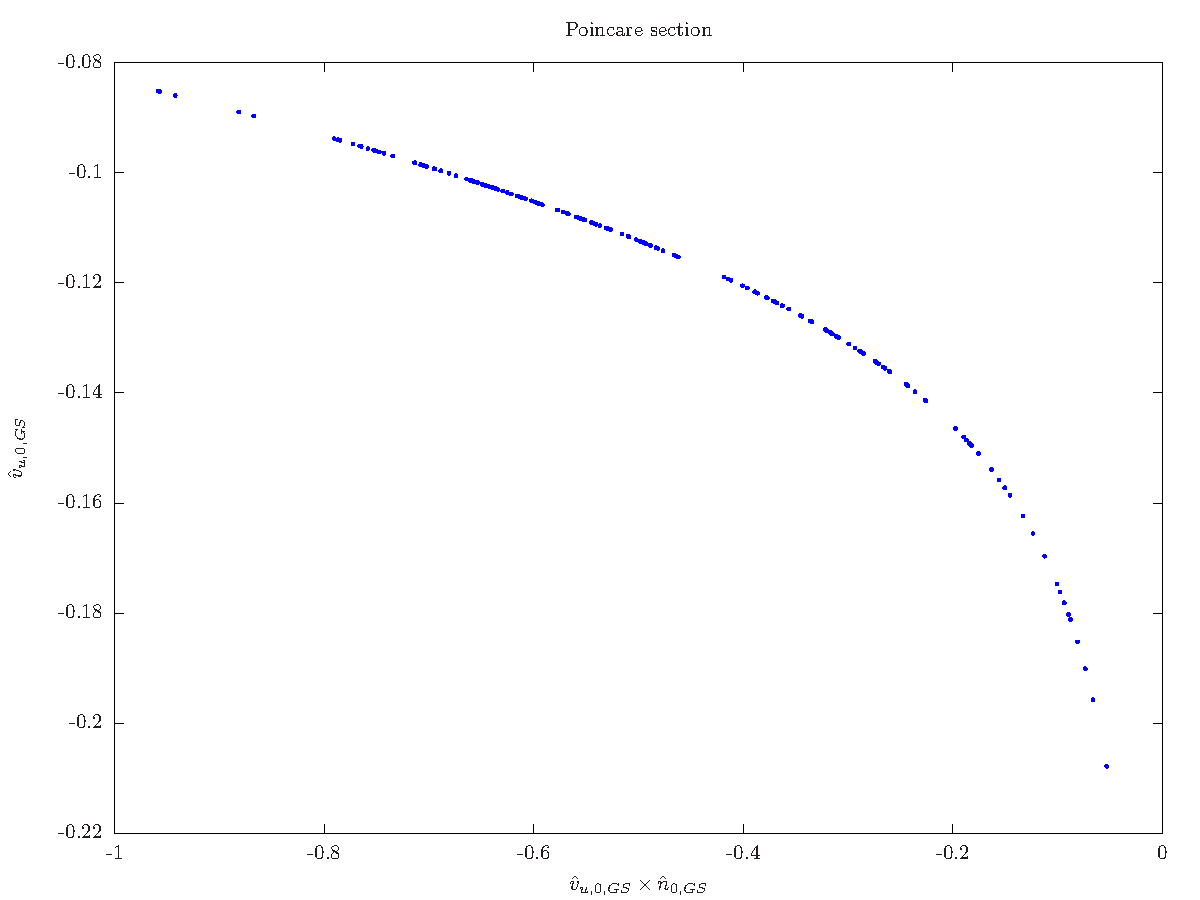
\includegraphics[width=0.8\textwidth]{BBPKpsect0}
  \end{center}
  \caption{
	Poincar\'e section plane which includes the \eqv\  \EQV{NameMe}
    and is perpendicular
	to the normal vector given in \refeq{eq:nhat0GS}.
    }
  \label{fig:BBPKpsect0}
\end{figure}

\begin{figure}%[ht]
  \begin{center}
  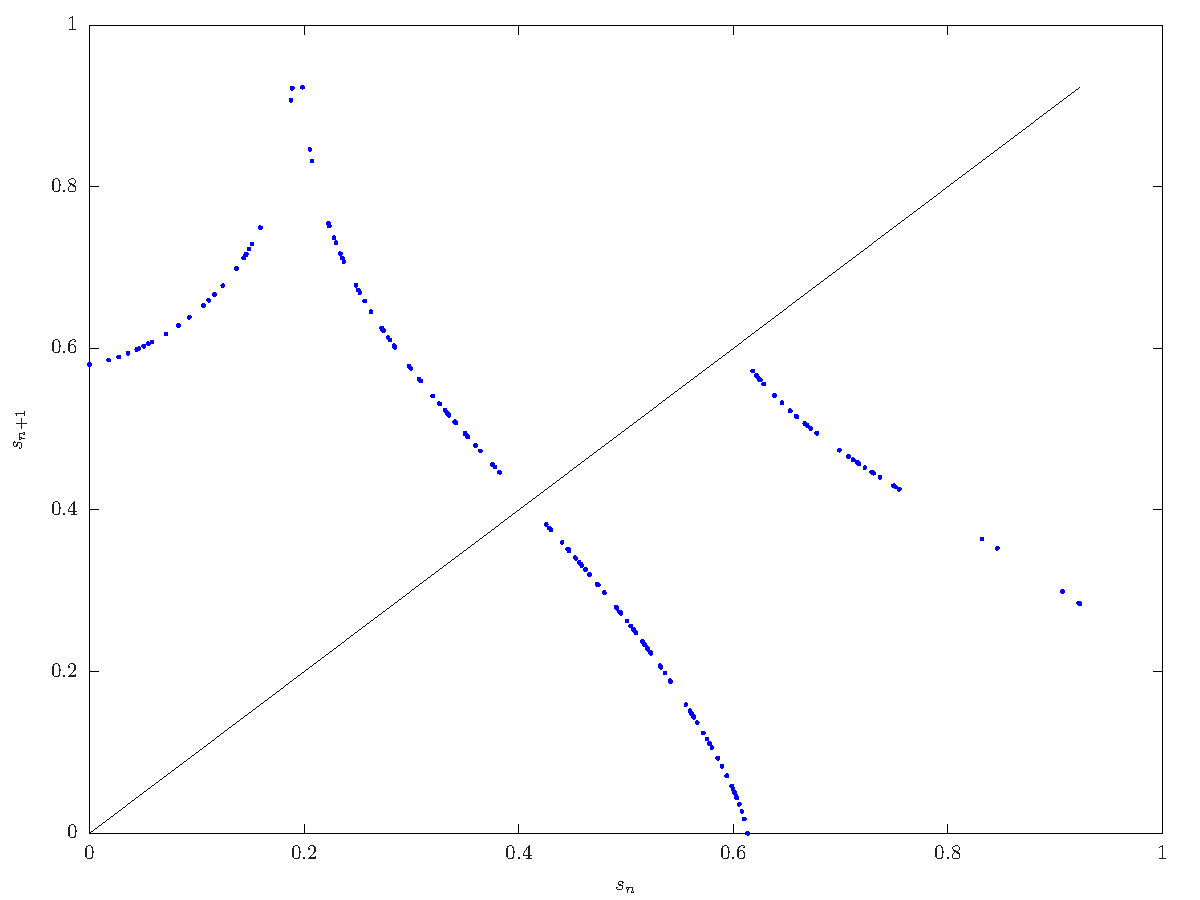
\includegraphics[width=0.8\textwidth]{BBPKretmap0}
  \end{center}
  \caption{
	Poincar\'e return map corresponding to the section in \reffig{fig:BBPKpsect0}.
    }
  \label{fig:BBPKretmap0}
\end{figure}

Poincare section plane \reffig{fig:BBPKpsect0} including the origin is
perpendicular to
\beq
	\hat{n}_{0,GS} = (0, -0.54030, 0.84147)
	\label{eq:nhat0GS}
\eeq
Poincar\'e section plane \reffig{fig:BBPKpsect1}\,(a) including the \reqv\ is
perpendicular to
\beq
	\hat{n}_{1,GS} = (0.977790, 0.184593, 0.099259)
	\label{eq:nhat1GS}
\eeq

\item[2013-10-02 Burak] Here (\reffig{fig:BBPKretmap0} and \reffig{fig:BBPKretmap0})
are the return maps of the Poincar\'e sections that I posted yesterday morning.
On both return maps, $s_n$ are arclengths along the respective Poincar\'e
section curves, starting from the \eqv /\reqv. Hopefully, I will blog \rpo s tomorrow.

\item[2013-10-03 Predrag] Cool - looks like return maps for the
Lorentz flow. You can already start nailing down you \rpo s using the
$\{0,1\}$ symbolic dynamics of \reffig{fig:BBPKretmap1} for initial
Newton guesses for \rpo s in the full 4\dmn\ \statesp. Plotting the
periodic points of the same \rpo s in   \reffig{fig:BBPKretmap0} will
help you elucidate the relation between the two sections - it looks
like \reffig{fig:BBPKpsect1}\,(a), suffices to explain everything.

\item[2013-10-03 Predrag] It will look even prettier if you - instead
of plotting the strange attractor - plot the unstable manifold ala
Adom Kamor. That will give you the return map(s) also outside the
strange attractor. As the attractor is exceedingly thin (estimate
that similarly to what is done in ChaosBook for the R\"ossler), your
initial guesses based on this 1\dmn\ return map will be very
accurate.

\item[2013-10-03 Predrag] Regarding return maps: please plot squares as squares.

\item[2013-10-03 Predrag] Low priority: it would be nice to plot the
Poincar\'e section planes in \reffig{fig:BBgramschmidt}, like it is
done for the symmetry-reduced Lorentz flow in ChaosBook.

\item[2013-10-03 Predrag] Re. figure source files  such as PSECT1.tex:
\begin{itemize}
  \item protests about lots of things it is missing?
  \item ``GNUPLOT: LaTeX picture with Postscript'' - does not it have an pdf option?
  Or I'm misreading the file...
  \item I recommend adding a comment line like one I added in LaTeX source
    to \reffig{fig:BBPKpsect1}\,(a), indicating the source for the figure -
    comes in handy later when editing, changing labels etc
\end{itemize}

\item[2013-10-03 Daniel] So I've been out of the loop... what still needs to be done?
Should I be trying to replicate Burak's work to see if I get the same thing? Is there
something that should be done in parallel? Should I try to do the whole Poincar\'e section,
return map, periodic orbit solver song and dance in invariant coordinates to see if we
get the same thing? Is there something more productive? Also, Burak, could you upload a file
with the relative equilibrium that you calculated specified to machine precision
(or at least more than 3-4 decimal places)? Might be useful to have it written down
in the $(x_1,x_2,y_1,y_2)$ basis.

\item[2013-10-07 Predrag] Burak's and Daniels outline of Das Artikel is
in \reffig{fig:131007outline}

\begin{figure}
  \centering
  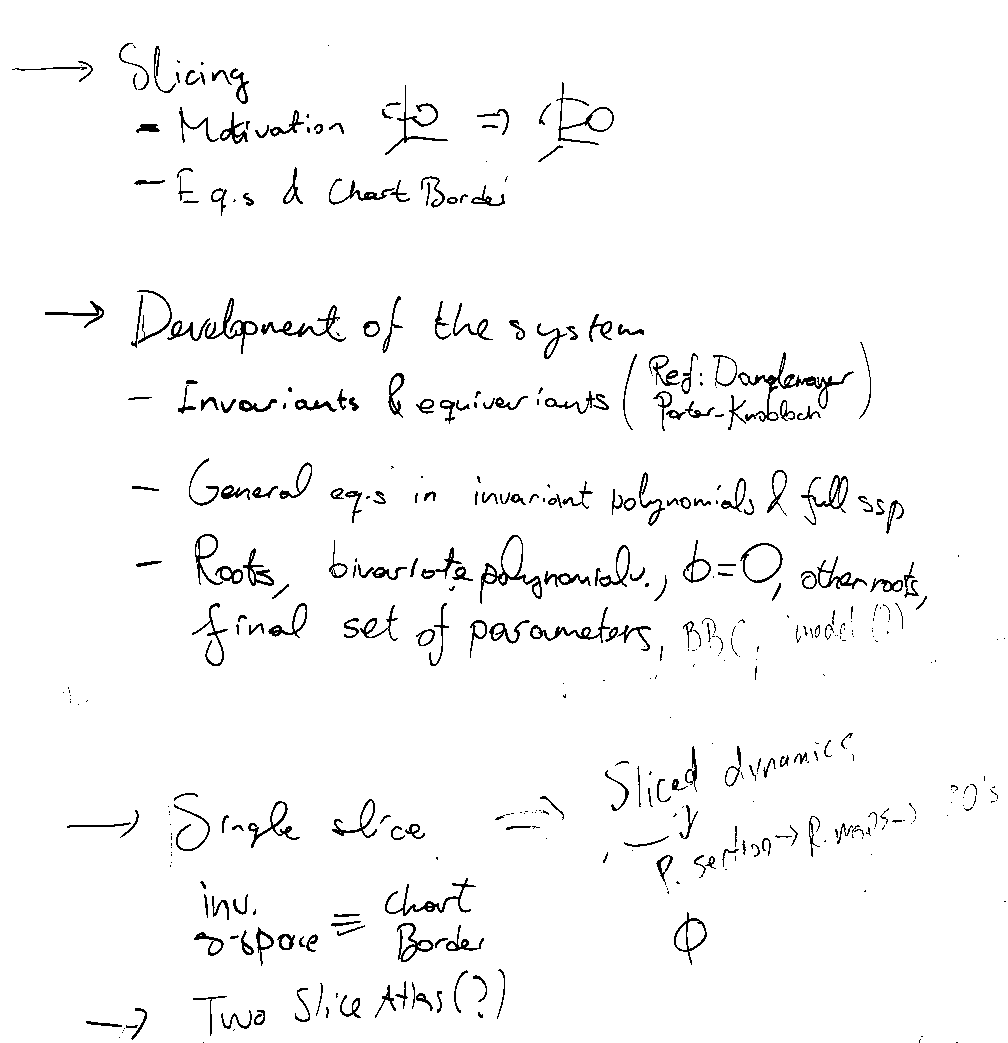
\includegraphics[width=0.6\textwidth]{131007outline}
  \caption{
Burak's and Daniels outline of Das Artikel.
  }\label{fig:131007outline}
\end{figure}


\item[2013-10-07 Burak] A short post about \rpo s:

After interpolating with cubic splines, the return map \reffig{fig:BBPKpsect1}\,(b)
looks like \reffig{fig:BBretmapinterp}. The intersection corresponds to a
\rpo\ which, in reduced space, looks like \reffig{fig:BBrpoGS}. I'm not blogging
the details, numbers etc. since they are subject to change now. I couldn't
yet figure out how to trim the white spaces around the figures, sorry, I will
fix that soon.

\SFIG{BBrpoGS}{}{
 A \rpo\ in the reduced space.
  }{fig:BBrpoGS}

\item[2013-10-07 Burak] After setting $b_{1,2} = 0$, the bivariate polynomials become:
\bea
	f(u,v) &=& -v (1+u a_2) c_1+u c_2 (u a_1+\mu _1 )
	\continue
    g(u,v) &=& v^2 c_1^2 e_2^2+ (2 v c_1+u c_2)^2 (-v c_1^2+ (-u+\mu _1 )^2))
	\label{eq:fgred1}
\eea
$f(u,v) = 0$ can be easily solved for $v$:
\beq
	v(u) = \frac{u c_2 (u a_1+\mu _1)}{(1+u a_2) c_1}
	\label{eq:vofu}
\eeq
Plugging this into $g(u,v)$ and simplifying gives:
\beq
	g(u) = u^2 c_2^2 \Bigg(\frac{e_2^2 (u a_1+\mu _1){}^2}{(1+u a_2)^2}+\Big(1+\frac{2 (u a_1+\mu _1)}{1+u a_2}\Big)^2
	       \Big((u-\mu _1){}^2-\frac{u c_1 c_2 (u a_1+\mu _1)}{1+u a_2}\Big) \Bigg)
	\label{eq:gu}
\eeq
Two-fold root at the origin can immediately be divided out. If one sets $a_1 = -1$,
which is the case with Daniel's parameters, $(u-\mu_1)$ also becomes a common
multiplier and hence, can be divided out. After doing that and some more manipulation we get
\beq
	g_{red}(u) = \frac{e_2^2 (u-\mu _1) (1+u a_2) + (u c_1 c_2 + (u-\mu _1) (1+u a_2)) (1+u a_2 - 2 (u-\mu _1 ))^2)}{(1+u a_2)^3} .
	\label{eq:gured}
\eeq
Now the roots of the \twoMode\ system is determined by the numerator of
the \refeq{eq:gured}, which is a quartic polynomial in $u$, hence, exactly solvable.
Observing that parameters $c_1,2$ only appears as $c_1 c_2$ in this equation,
I tried to further simplify the parameters by setting $c_2 \to 1$ and $c_1 \to c_1 c_2$ .
This scaling preserves chaos. After this, parameters which are set to 1s and
0s are:
\beq
	\mu_2 = 1, a_1 = -1, b_1 = 0, b_2 = 0, c_2 = 1, e_2 = 1
	\label{eq:1sand0s}
\eeq
There are three parameters left to determine. I rounded the reamining parameters
to 2 decimals and got the following set:
\bea
	\mu_1 = -2.8 , a_2 = -2.66 , c_1 = -7.75
	\continue
	\mu_2 = 1, a_1 = -1, b_1 = 0, b_2 = 0, c_2 = 1, e_2 = 1
	\label{eq:parsc2red}
\eea
The flow with these parameters is nicely chaotic, I actually got a radial
Poincar\'e return map in the invariant polynomial basis qualitatively very
similar to the one I got in the reduced \statesp\ with the previous parameters.
There are analytical expressions for the roots of quartic polynomials, however,
they are too long and I could not make a sense out of them. With \refeq{eq:parsc2red}
Numerical roots of the quartic polynomial are:
\bea
	u &=& -5.52172
	\continue
		   &=& -0.991847 - 0.14571 i
	\continue
		   &=& -0.991847 + 0.14571 i
	\continue
		   &=& 0.19357
	\label{eq:uroots}
\eea
With the divided out roots (2 at $u=0$ and 1 at $u=\mu_1$) and the one at the
infinity ($v = -\mu_2 / \b_2$), we have all the roots now \BBedit{(This may be
wrong. There might be another root that is sent to infinity by setting $b_1 = 0$,
since the original bivariate polynomials are of degree 2 and 4 and the root
at $v = -\mu_2 / \b_2$ is already divided out. I cannot immediately see this, however,
it is not important once the choice of 0s and 1s \refeq{eq:1sand0s} is made, after
that one can get all the roots analytically.)}. Only the positive real root listed
above, along with the root at the origin, directly influences the flow in
the full \statesp . I'm not able to comment on the possible intermittency
right now.

\item[2013-10-07 Predrag]
Why does the front page of the paper have only the title and authors?
\item[2013-10-07 Burak]
{It's something weird with the Chaos style file and the fact that
    we have been compiling as preprint instead of reprint. If you toggle
    this it looks fine. Do we have a plan for where we want to submit
    this?}
\item[2013-10-10 Predrag]
Currently I'm thinking of Chaos, as it is a sequel (should have been
a prequel) to \refref{atlas12}, but we could send it someplace else,
if you wish.

\item[2013-10-10 Predrag]
Please always plot square as a square, not as a rectangle,
as currently in
\reffig{fig:BBPKretmap0}, \reffig{fig:BBPKpsect1}\,(b) and
\reffig{fig:BBretmapinterp}.

\item[2013-10-11 Predrag]
We still have another case to investigate, the Dangelmayr
normal form system,\rf{Dang86} with the parameters $\{e_1,e_2\}=\{0,0\}$
and the $\On{2}$ symmetry. We need it, as this is the symmetry of \KS\
as well. The system \refeq{eq:DangSO2} then has also a discrete symmetry
(complex conjugation), and a 2\dmn\ invariant subspace spanned by
$=\{\Im{z}_1,\Im{z}_2\}=\{x_2,y_2\}$.
    \PC{please recheck}
That should lead to `preperiodic orbits' discussed in \refref{SCD07}.
We should probably quotient the reflection symmetry, work in a
fundamental domain.

\item[2013-10-12 Burak]
I worked/experimented on $e_{1,2} = 0$ case and could not find a chaotic
flow. For now, I have only one thing to say about what won't work:

It is impossible to get anything chaotic by taking \refeq{eq:parsc2red}
and setting $e_2$ to 0. Velocity function for the invariant coordinate q,
after substituting 0s and 1s \refeq{eq:1sand0s} is
\beq
	\dot{q} = q u (-2 + a_2) + q(1+2 \mu_1)
	\label{vq1sand0s}
\eeq
Since $u$ always takes positive values and the parantheses in this equation
are both negative for the parameter choice \refeq{eq:parsc2red}, the flow
always approaches to $u=0$. Once this happens, \twoMode\ flow becomes effectively
2 dimensional since two of the invariant coordinates determine the third one
through the syzygy. I experimented with other parameters but could not find
anything interesting yet.

\item[2013-10-15 Burak]
I have been trying to find a parameter set with $e_2 = 0$ for which the flow
is chaotic. So far, I could not find chaos, but I found something that might
be promising. After a lot of analytical trials and getting nothing useful,
I went back to my older parameters and set $e_2 \rightarrow 0$ and varied
other parameters and finally got:
\bea
	\mu_1 &=& 2 , a_1 = 0.41 , b_1 = -1.7, a_2 = 0.16, b_2 = -0.05
	\continue
	c_1 &=& 1, \mu_2 = -1, c_2 = -1, e_2 = 0
	\label{eq:parsO2}
\eea
Flow in the invariant polynomial basis looks like \reffig{fig:BBO2invpol}.
It converges to a limit cycle. I'm blogging this because the limit cycle might
be unstabilized by tweaking the parameters \refeq{eq:parsO2}.
\SFIG{BBO2invpol}{}{
 Flow with parameters \refeq{eq:parsO2} on the invariant polynomial basis.
  }{fig:BBO2invpol}

I also computed the flow in the full \statesp\ (\reffig{fig:BBO2fullssp}) and symmetry reduced using
the magic slice (\reffig{fig:BBO2gramschmidt}) without quotienting the reflection symmetry (don't know how to
do it yet). Both post processing and integration on the slice methods give
the same results up to small numerical errors.
\SFIG{BBO2fullssp}{}{
 Projection of the flow with parameters \refeq{eq:parsO2} in the full \statesp.
  }{fig:BBO2fullssp}
\SFIG{BBO2gramschmidt}{}{
 Symmetry reduced flow with parameters \refeq{eq:parsO2} on the Gram-Schmidt basis.
  }{fig:BBO2gramschmidt}

\item[2013-10-15 Burak]
A new set of parameters for \refeq{2mode4D}, \On{2}-equivariant case:
\bea
	 a_1 &=& 0.47
	\continue
	\mu_1 &=& 1, b_1 = -1, c_1 = 1, \mu_2 = -1, a_2 = 0, b_2=0 , c_2 = -1, e_2 = 0
	\label{eq:parsO2a1only}
\eea
This, I think, is the simplest looking set of parameters we have found so
far. Three of the original nine parameters are set to zero and five of them
are set to either 1 or -1. For smaller values of $a_1$, The flow in the invariant
space converges to a limit cycle as in \reffig{fig:BBO2invpol}, and for the
larger values it approaches to an \eqv\ (might be a \reqv\ in the equivariant
 \statesp ). With $a_1 = 0.47$, flow in the invariant space looks like
\reffig{fig:BBO2invpola1only}.

I also computed the full \statesp\ flow (it's a mess) and symmetry reduced it
without quotienting the reflection symmetry. I'm posting the reduced flow on
the Gram-Schmidt coordinates of \refeq{eq:GramSchmidtBasis} for a short time
interval in \reffig{fig:BBO2a1onlygramschmidt}.  It's looks a bit messy if
I plot it for the entire flow ($t_{final} = 500$). Topologically, it's like a
torus bent in a shape similar to that of \reffig{fig:BBO2gramschmidt}

Please double-check the parameters and the existence of chaos. If this looks
promising, please make suggestions about the next steps, I'm guessing the
first one to be quotienting the reflection symmetry. It is possible to get
all the \eqva\ in the invariant space, because the parameters are rather simple.

\SFIG{BBO2invpola1only}{}{
 Flow with parameters \refeq{eq:parsO2a1only} on the invariant polynomial basis.
  }{fig:BBO2invpola1only}

\SFIG{BBO2a1onlygramschmidt}{}{
 Symmetry reduced flow with parameters \refeq{eq:parsO2a1only} on the Gram-Schmidt basis.
  }{fig:BBO2a1onlygramschmidt}

\item[2013-10-21 Burak]
I am starting moving the code from Octave/Matlab to NumPy, completed slicing,
Poincar\'e sections are the next. The previous code was using slow integrators
and solvers written by me. This one mostly uses built in NumPy functions,
which are much faster. I did this transformation mainly to speed up things
to make unstable manifold algorithm feasible to run. Also, NumPy has powerful
plotting tools so I will be able to plot Poincar\'e section planes soon.

I'm committing the code, a README file and bash scripts to run the programs at:
\texttt{blog/burak/PorterKnobloch/python}.
I prepared small scripts to install the required packages for Linux users,
so if you want to re-run something, it should be really easy to do it on Linux.
That is the way of generating 3D interactive figures for now, I will try to
find a web based way of sharing rotatable figures.

This transition is temporarily slowing my progress down but it will ultimately
be speed it up.

\item[2013-10-23 Predrag] Some thoughts on the days'
Poincar\'e section \reffig{fig:BBO2Psect}\,(b):
% yet-unblogged  \texttt{psectgs.png}
it looks like a very slow
transient to cycle of discrete time 13. Would be impossible to see
that without Poincar\'e section... Invariant polynomial representation
seems useless.
% Is the plane in \reffig{fig:BBO2Psect}\,(a)
%\texttt{gramschmidtandpsect.png}
% really a
% Poincar\'e section, and not the invariant subspace / \chartBord\
% \refeq{eq:chartBord}? If it is the section, looks like not a good
% choice.
You want to mark \reqva\ and their eigenvectors, then have
the section go through the important \reqv, traverse the complex
eigenvector pair plane.

To reveal the attractor, you want to first run it for a long time,
then start plotting. Possible genesis; there was once a stable Hopf
limit cycle bifurcated off an \rpo\ gone unstable. A shorter period
stable Hopf limit cycle bifurcates off next; they mode-lock with
discrete time ratio $m/13$, $m$ relative prime to 13, \ie,
$m=1,2,\cdots,12$. Not sure about this at all, but your system is
sure a rare beast :)

\begin{figure}%[H]
\centering
 (a) 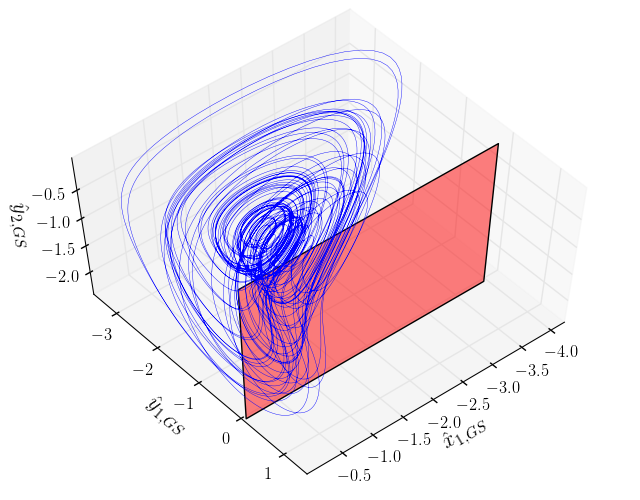
\includegraphics[width=0.35\textwidth]{BBO2gsandpsect}
 (b) 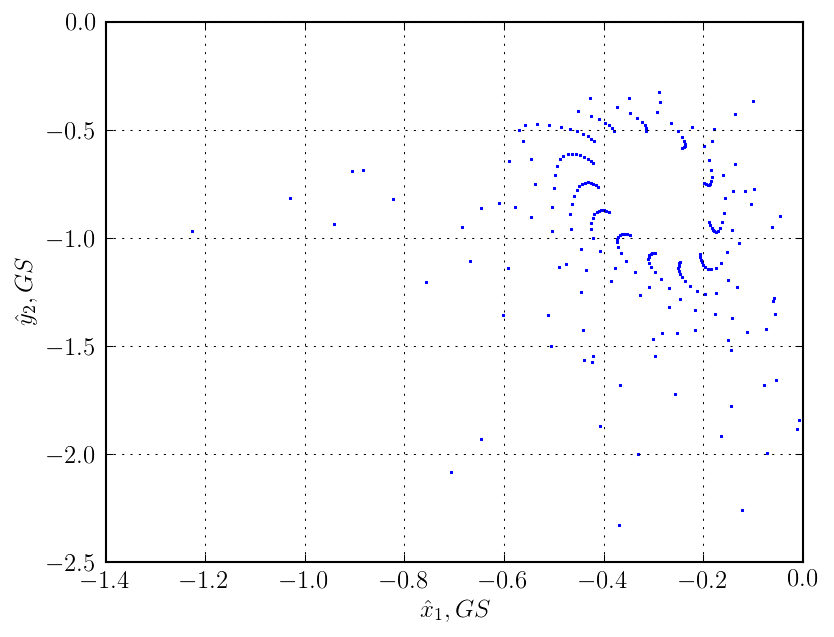
\includegraphics[width=0.35\textwidth]{BBO2psectgs}
\caption{(a) Reduced flow (blue) on the Gram-Schmidt basis and the Poincar\'e
section hyperplane. (b) Corresponding Poincar\'e section. Parameters \refeq{eq:parsO2a1only}
}
\label{fig:BBO2Psect}
\end{figure}

\item[2013-10-23 Burak] The \On{2} invariant system with the parameters \refeq{eq:parsO2a1only}
has seven roots on the invariant polynomials:
\bea
	(u,v,w) &=& (0,0,0)
			\continue
			&=& (16.6667,8.33333,-16.6667) \mbox{(double)}
			\continue
			&=& (-1.12714,4.16894,-8.33787)
			\continue
			&=& (0.270366,0.239869,-0.479739)
			\continue
			&=& (-1.38372,1.26085,-2.5217)
			\continue
			&=& (1.09745,0.793116,-1.58623)
	\,.
\label{eq:BBO2roots}
\eea
None of these but the origin has a real correspondence in the full \ssp\
(This result badly needs to be double checked). I let Mathematica try to find
the real $(x_1,x_2,y_1,y_2)$ that solves \refeq{eq:PKinvxirels} also did an
independent Newton search, none of which found a solution. For now, I believe,
this system has no \reqv.

Having no interesting \reqv, I then decided on trying a Poincar\'e section
including the origin and its unstable direction which, on Gram-Schmidt basis
simply is $\sspRed_{1,GS}$ direction. This Poincar\'e section is shown in
\reffig{fig:BBO2Psect}. In \reffig{fig:BBO2Psect}, initial condition is a
point very close to the origin. I then started from the final point of this
simulation and run another 1000 time units and computed the Poincar\'e section
again (\reffig{fig:BBO2Psect2}). I think this 13-cycle on the Poincar\'e
section is the bifurcation of the limit cycle of \reffig{fig:BBO2gramschmidt},
however, since the attractor is not thin, I'm not able to make an arc-length
return map as I did for the previous case. I'm thinking whether it would be possible
to do a `local symmetry reduction' since all the points on the Poincar\'e
section look like they have a symmetry of an ellipse, if that symmetry
can be reduced then it may look like it's converging to a single point. While
writing these, I did a much longer run, which made the squid convergence more
apparent \reffig{fig:BBO213cycle}, however, as you can see there are more legs
in this picture, which makes me think that this might be converging to a single
limit cycle, but very slowly.

\begin{figure}%[H]
\centering
 (a) 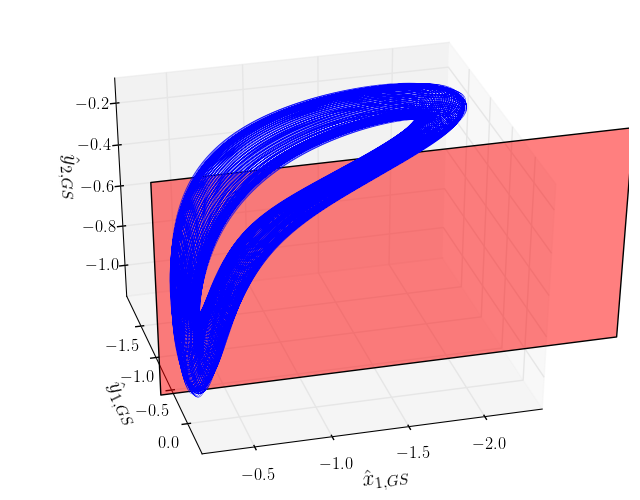
\includegraphics[width=0.35\textwidth]{BBO2gsandpsect2}
 (b) 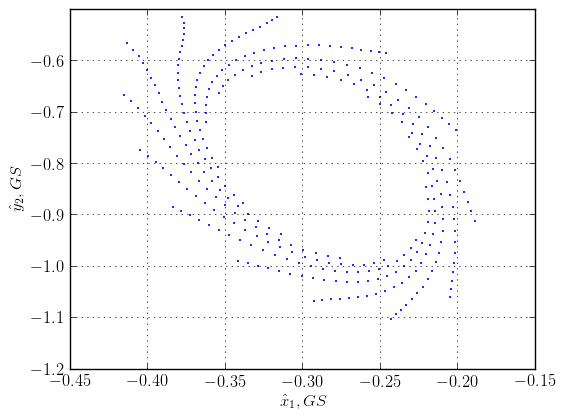
\includegraphics[width=0.35\textwidth]{BBO2psectgs2}
\caption{(a) Reduced flow (blue) on the Gram-Schmidt basis and the Poincar\'e
section plane. (b) Corresponding Poincare\'e section. Parameters \refeq{eq:parsO2a1only}.
}
\label{fig:BBO2Psect2}
\end{figure}

\SFIG{BBO213cycle}{}{
 Convergence to an apparent 13-cycle on the Poincar\'e section
 of \reffig{fig:BBO2Psect}.
  }{fig:BBO213cycle}

\item[2013-10-24 Burak] After playing with $a_1$ and getting different sorts
of cycles on the Poincar\'e section of \reffig{fig:BBO2Psect} and \reffig{fig:BBO2Psect2},
I decided to do it systematically. I took 1000 equally spaced values between
$0.45$ and $0.49$ for $a_1$ and integrated the flow for $1000$ time units,
computed the Poincar\'e section for the last $500$ time units of the simulation
and plotted the values on the Poincar\'e section individually against the varying parameter.
Resulting figure: \reffig{fig:BBO2bifurcation}. Looking at this, I think the
chaotic behavior is somewhere around $a_1 = 0.475$.

\begin{figure}%[ht]
  \begin{center}
  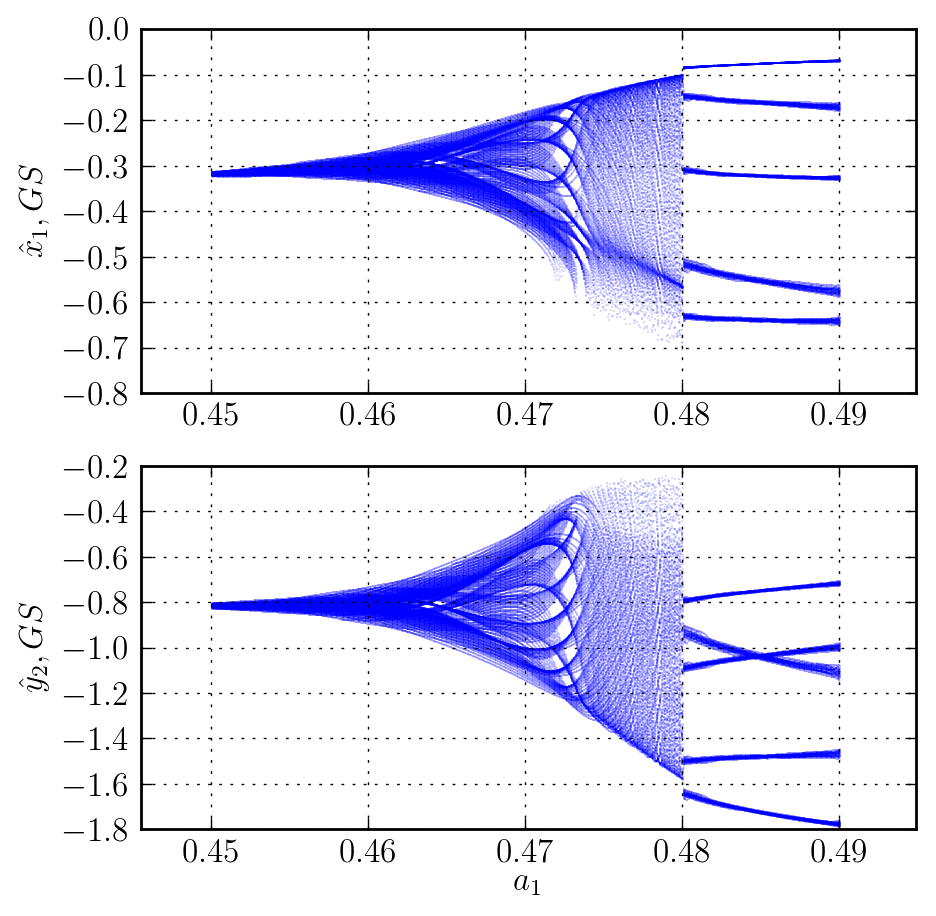
\includegraphics[width=0.8\textwidth]{BBO2bifurcation}
  \end{center}
  \caption{
Bifurcation diagram for the Poincar\'e section (see
\reffig{fig:BBO2Psect}\,(b), \ref{fig:BBO2Psect2}\,(b), and
\ref{fig:BBO213cycle} 	for the section
evaluated at $a_1 = 0.47$)
of the \On{2}\ invariant flow with parameters \refeq{eq:parsO2a1only},
$a_1$ varying.
    }
  \label{fig:BBO2bifurcation}
\end{figure}

\item[2013-10-25 Predrag]
Poincar\'e section \reffig{fig:BBO2Psect}\,(b) seems to be converging to
a 13-cycle, but it does not seem to do so in the other, longer time
sections? It seems that the dynamics is converging to a torus of neutral
stability, leading to excruciatingly slow convergence to it?

\item[2013-10-28 Burak] % Sorry for late blogging, I was in the TA duty hell.
The region of the bifurcation diagram \reffig{fig:BBO2bifurcation} which I
thought was chaotic, unfortunately (or maybe not) was not chaotic, in fact, if
I counted correctly, it is a 68-cycle. I am arriving the 'not chaotic' conclusion
by observing that long runs of the system is confined on the surface of a torus
in the symmetry reduced space, hence the dynamics is 2 dimensional so it
cannot exhibit chaos. I also checked variation of $x$ with time and saw recurrence
with period approximately 472 time units. Nevertheless, I think, this is still
interesting dynamics and it demonstrates the importance of the symmetry reduction.
For $a_1 = 0.4775$, Poincar\'e section is shown in \reffig{fig:BBO2psectgsa1eq0475}

\SFIG{BBO2psectgsa1eq0475}{}{
 A \rpo\ with a very long period ($\period{} \approx 472$) on the
 Poincar\'e section of \reffig{fig:BBO2Psect} in the reduced \statesp.
 Parameters \refeq{eq:parsO2a1only}, with $a_1 = 0.4775$.
  }{fig:BBO2psectgsa1eq0475}

\item[2013-10-28 Burak] I reduced the reflection symmetry as follows:
I first computed the reduced dynamics within the slice, then found the points
on the trajectory with $y_2(t*) < 0$, and then mapped these points as
\bea
 x_2(t^*) & \rightarrow & -x_2(t^*) ,
 \continue
 y_2(t^*) & \rightarrow & -y_2(t^*) .
 \label{eq:refred}
\eea
This operation corresponds to complex conjugation of the initial mode amplitudes.
Result of this operation is in \reffig{fig:BBO2onslicerefred}. I didn't find
this plot particularly informative but if you would like to rotate and zoom
in to this plot, please run

\texttt{bash O2integrateonslice.sh}

in the folder:

\texttt{blog/burak/PorterKnobloch/python/}

\item[2013-10-29 Predrag]
Comparing with \reffig{fig:BBO2a1onlygramschmidt},
\ref{fig:BBO2Psect}\,(a) and \ref{fig:BBO2Psect2}\,(a) I see your
point - it does not look good when orbit is discontinuously injected
in a conter-moving direction. Usually orbits are self-dual under
reflection (in which case you would find this more insightful) or
come as dual pairs; where is the \refeq{eq:refred}-reflected dual of
your orbit in the above figures? There might be something about
\On{n} vs. \SOn{n} that we are misunderstanding...

\item[2013-10-29 Predrag] Regarding Poincar\'e section of
\reffig{fig:BBO2Psect} - I seem to remember that we argued that
Poincar\'e sections should be discrete symmetry invariant (? how
would one guarantee transversality of section crossings then? have to
reread ChaosBook.org suggestions plus \refref{atlas12} myself :).
That would put the section plane into $(x_2,y_2)=(0,0)$. In any case,
it might be useful to mark those points in
\reffig{fig:BBO2onslicerefred} as red dots, to see where the
reflection happens.


\SFIG{BBO2onslicerefred}{}{
	Dynamics in the reduced \statesp\ with reflection symmetry reduced to mapping
	solutions to the half-space with $y_2 > 0$ as described in \refeq{eq:refred}.
    Compare with \reffig{fig:BBO2a1onlygramschmidt}, \ref{fig:BBO2Psect}\,(a) and
    \ref{fig:BBO2Psect2}\,(a).
    Parameters \refeq{eq:parsO2a1only}, with $a_1 = 0.4775$.
  }{fig:BBO2onslicerefred}

\item[2013-10-28 Burak] Figure 5 in Porter-Knobloch paper\rf{PoKno05}
shows a chaotic flow with an attractor topology very similar to what
we got in \reffig{fig:BBunstablevectors}. There, they are using some kind of a
symmetry invariant basis, which, I suspect may be equivalent to the `magic slice'.
I thought it would be a good start to simulate the system with their parameters,
however, there is no direct mapping of their parameters to ours since we don't
have the most general 2-mode system here. I'll work on this correspondence in
more detail.

\item[2013-10-28 Burak] As discussed in [2012-04-29 Daniel to Gang], our current
mapping from two complex modes to the real valued 4D \statesp\ is as follows:
\bea
	z_1 &=& x_1 + i x_2 ,
	\continue
	z_2 &=& y_1 + i y_2 .
	\label{eq:C2toR4}
\eea
While this is similar to the mapping that you used for the {\cLe},
I think $z_j = x_j + i y_j$ is more informative since it is straightforwardly
generalizable to the more than 2 mode cases with $x_j$ and $y_j$  respectively
corresponding to the real an imaginary parts of the $j^{th}$ mode. I also
checked the previous two mode literature \refref{Dang86} and \refref{PoKno05}
do not have a mapping to real variables like \refeq{eq:C2toR4}. If it makes
sense to you, I am suggesting using $z_j = x_j + i y_j$ for  $\mathbb{C}^2$
to $\mathbb{R}^4$ mapping, I can do all the changes in Das Artikel and the codes
in approximately an hour.

\item[2013-10-29 Predrag] I bow my head in shame - ``follow the
precedent'' creed makes no sense here, {\cLe} has two $m=1$
representations, while here we care about different $m$'s. If you
have the strength, (re)introduce the sensible notation, please.
\\
{\bf [2013-10-30 Burak]} Implemented the redefinitions, in the
main \texttt{2modes.tex} file only.



\item[2013-10-03 Evangelos to Burak]
I hate it to sound like Kassandra, but I do not see where 'magic' in
your slice comes from. Using the non-magic template
$\slicep=\{0,\sqrt{2},0,0,0\}$ for the {\twoMode} system gives a figure
equivalent (see \reffig{fig:2modesSlice1f}) to what you get if you
use $\slicep=\{1,1,0,0\}$. To me this is no surprise: since your flow
is rotationally symmetric, any two templates that can be rotated into
each other will give you equivalent results. Note that the equation
for the slice could be written as $\Re z_1=0$, and that we might as
well have used template $\slicep=\{0,1,0,0\}$ since this also leads
to the same condition. Singularities occur here only if $z_1=0$,
which corresponds to the invariant subspace of the 2modes flow, and
thus we are safe.

%%%%%%%%%%%%%%%%%%%%%%%%%%%%%%%%%%%%%
\SFIG{2modesSlice1f}{}{
Symmetry reduced {\twoMode} system for $\mu_1=-2.8023, \mu_2=1,
a_1=-1, a_2=-2.6636, b_1  = 0, b_2=0, c_1=-4.1122, c_2=1.8854, e_1=0,
e_2=1$. Using moving frames method with $\slicep=\{0,\sqrt{2},0,0\}$.
Compare with \reffig{fig:BBunstablevectors} (E. Siminos 2013-10-03).
}{fig:2modesSlice1f}
%%%%%%%%%%%%%%%%%%%%%%%%%%%%%%%%%%%%%

\item[2013-11-04 Burak to Evangelos]
I agree that \template s $\slicep = \{1,1,0,0\}$ and $\slicep = \{0,1,0,0\}$
are geometrically equivalent to each other and they would yield similar results
using \mframes, however, I would expect you to be in trouble if you integrate
within the \slice\ of $\slicep = \{0,1,0,0\}$ .

\item[2013-11-03 Predrag]
In \refref{KreEck13} the claim is made that the `{\mconn}'
\beq
	\dot{\ssp}_\perp = \vel_\perp(\ssp) = \vel(\ssp)
    - \frac{\groupTan(\ssp) \cdot \vel(\ssp)}{\groupTan(\ssp)^2}
      \, \groupTan(\ssp)
\ee{transvFlow}
`calms' the flow. It is very easy for you to implement it for the full
\statesp\ flow of \reffig{fig:BBO2fullssp}, and see what you get. My
expectation is the flow will not be very different, as the {\mconn} is
not a symmetry reduction scheme, but merely a different way to explore
the same group orbit of the flow in the full \statesp. Another line of
the argument:

In the presence of an $N$-continuous parameter symmetry, each \statesp\
point $\ssp$ owns $(N\!+\!1)$ tangent vectors: one $\vel(\ssp)$ along the
time flow $\ssp(\zeit)$ and the $N$ group tangents  $\groupTan_1(\ssp),
\, \groupTan_2(\ssp) ,\,\cdots, \groupTan_N(\ssp)$ along infinitesimal
symmetry shifts, tangent to the {$N$\dmn} group orbit $\pS_\ssp$.
A group tangent and the \statesp\ flow velocity at an instant $\ssp=
\ssp(\zeit)$ of a typical turbulent state are not likely to be close
to parallel. For fluid flows the \statesp\ is high dimensional, and
if the angles $\theta_j (\zeit)= \theta_j (\ssp(\zeit))$ between them
\beq
\cos \theta_j (\ssp) =
    \frac{\vel(\ssp)\cdot\groupTan_j(\ssp)}
         {\norm{\vel(\ssp)}\norm{\groupTan_j(\ssp)}}
\ee{typTangAngle}
are probabilistically distributed, two such vectors in high
dimensional \statesp\ are mostly nearly  orthogonal, and there is
no `calming' effect in the {\comovframe}.

Maybe a time series plot of \refeq{typTangAngle} would also be
informative...

\item[2013-11-05 Burak] I implemented in {\mconn} \refeq{transvFlow} by integrating \refeq{transvFlow}
for \On{2}-equivariant case and plotted trajectories for a \rpo\ in \reffig{fig:BBO2RpoSspComovSlice}.
\\
{\bf [2013-11-05 Predrag]} \PCedit{($\RPO{01}$ repeated how many periods?)}

\begin{figure}%[H]
\centering
 (a) [PLOT] $~~~~~~~~~~~~~~~~~~$
 (b) 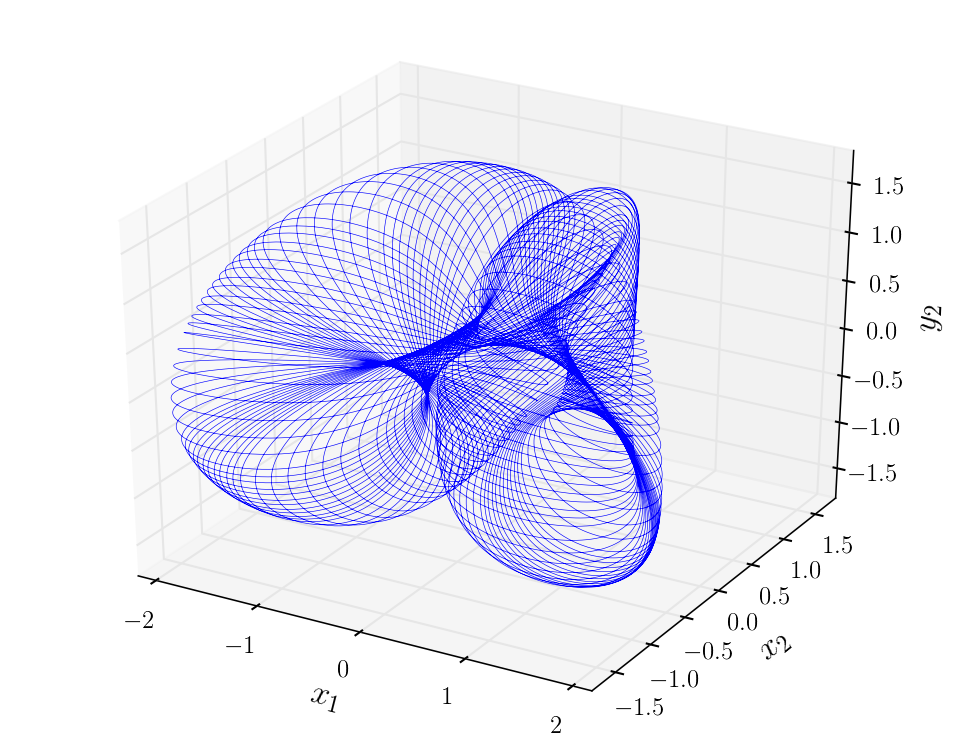
\includegraphics[width=0.3\textwidth]{BBO2a1045rpossp}
 \\
 (c) 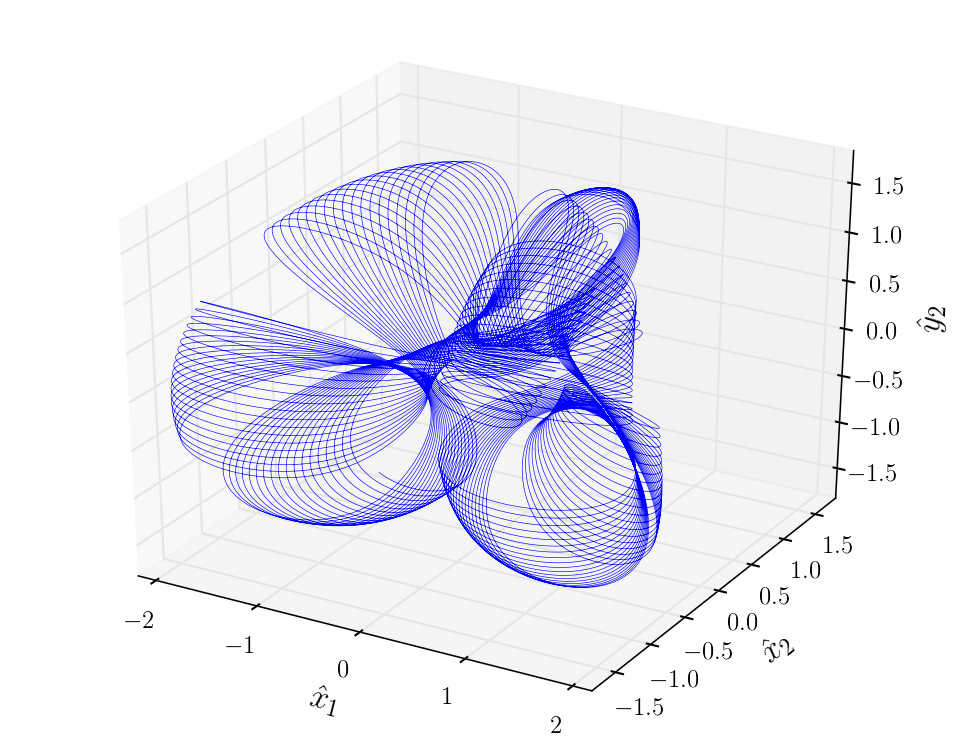
\includegraphics[width=0.3\textwidth]{BBO2a1045rpocomov}
 (d) 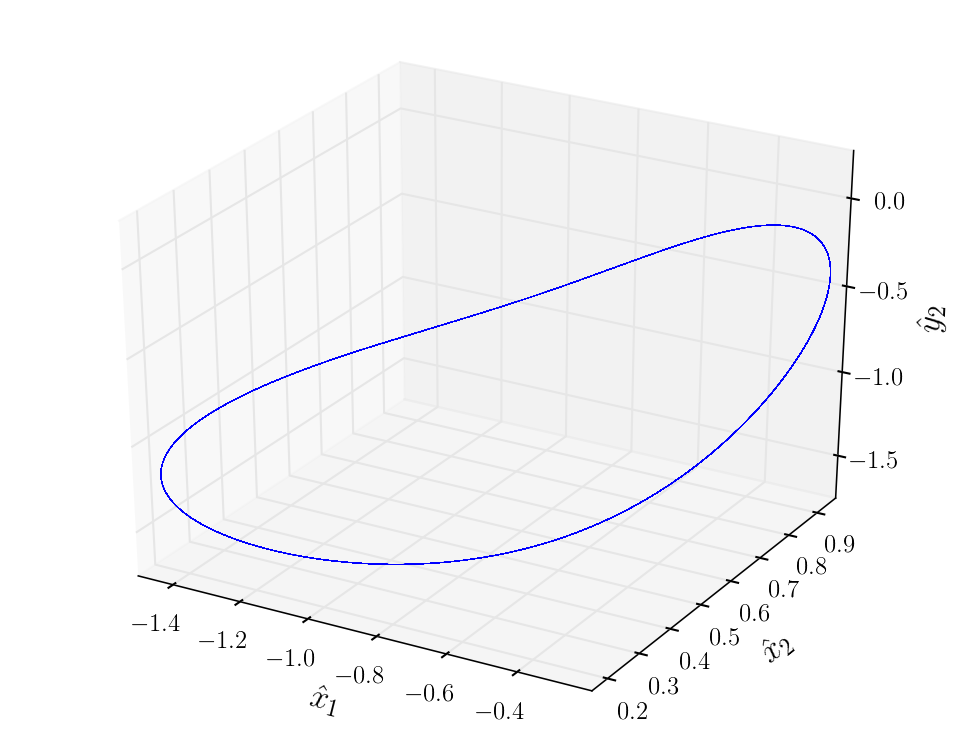
\includegraphics[width=0.3\textwidth]{BBO2a1045rposlice}
\caption{
(a) A single traversal of \rpo\ \cycle{01}, period $\period{01}=???$,
shift $\shift_{01}=???$ (the 2-cycle of the Poincar\'e return map
such as \reffig{fig:BBretmapinterp}). This is a $3D$ projection of the
full $4D$ \statesp\ \On{2}-equivariant {\twoMode} flow
\refeq{2mode4D}.
(b) \Rpo\ \cycle{01} integrated for  ?? periods $\period{01}$. It
explores ergodically the group orbit of the \rpo, a $2D$ invariant
torus embedded in $4D$. Other projections on any three coordinates
$\{x_1,y_1,x_2,y_2\}$ are qualitatively similar.
(b) The same trajectory computed integrating the {\comovframe}
transformed equations \refeq{transvFlow}. As the {\mconn} is not a
symmetry-reduction method, the trajectory explores ergodically the
same invariant torus, but with a different shift $\shift_{10}^{cm}=???$
per period.
(c)  In the \slice\ this trajectory retraces the corresponding \po.
Parameters: \refeq{eq:parsO2a1only} with $a_1 = 0.45$.
}
\label{fig:BBO2RpoSspComovSlice}
\end{figure}


\item[2013-11-11 Burak] After trying to improve the numerical precision of
the \reqv\ in \reffig{fig:Set1} I realized that it actually is not a \reqv ,
I'll try to explain why: I thought the second of the roots of invariant polynomials
that I listed in \refeq{eq:eqvaset1} would have a correspondance in the equivariant
\statesp\ provided by $u, v > 0$, however, the condition is more strict than that.
Let's write down the equations that connects the state variables to the invariant polynomials:
\bea
	u &=& x_1^2 + y_1^2,
	\continue
	v &=& x_2^2 + y_2^2,
	\continue
	w &=& 2 x_1^2 x_2 - 2 y_1^2 x_2  + 4 x_1 y_1 y_2,
	\continue
	q &=& -2 x_1^2 y_2 + 2 y_1^2 y_2 + 4 x_1 x_2 y_1
	\label{eq:ssp2invpol}
\eea
Now, since these equations are invariant under $\SOn{2}$ operations, if there is
a solution $x = (x_1, y_1, x_2, y_2)$ to them for a particular $(u,v,w,q)$ then,
all the vectors $\LieEl(\theta)x, \theta \epsilon {0,2 \pi}$ are also solutions.
Thus, as a particular solution, we can choose the one within the \slicePlane\ of
$\slicep = (1,1,0,0)$, namely $x = (x_1, x_1, x_2, y_2)$. Plugging this candidate
solution into \refeq{eq:ssp2invpol}, we get:
\bea
	u &=& x_1^2 + x_1^2,
	\continue
	v &=& x_2^2 + y_2^2,
	\continue
	w &=&  4 x_1^2 y_2,
	\continue
	q &=&  4 x_1^2 x_2
	\label{eq:ssp2invpolwithinslice}
\eea
From the first relation we get $u=2x_1^2$, plugging this into the last two,
we get $x_2 = q/2u$, $y_2 = w/2u$, finally plugging these into the second equation
we obtain a condition for an \eqv\ in the invariant polynomials to have a
corresponding \reqv\ in the equivariant \statesp:
\beq
	4 u^2 v = w^2 + q^2
	\label{eq:reqvcond}
\eeq
The second root in the list does not satisfy \refeq{eq:reqvcond}, however,
LHS of equation is 0.023101 while RHS is 0.022620. The \statesp\ point
$x_0 = (−0.31056, −0.31056, −0.04191, −0.38981)$ which I thought was a solution to
\refeq{eq:ssp2invpolwithinslice} was in fact not a solution, but a minimum and
the red curves in \reffig{fig:Set1}(a,b) were not an unstable \reqv\ but
trajectories effected by some sort of an intermittency.

This, I think, is interesting, but it also proves that my previous Jacobian calculations in
[2013-09-28 Burak] were not accurate. If I compute the Jacobian as if this
orbit is periodic and look for the eigenvalues, I still get something close to 1
on the group tangent direction, however, the accuracy is low to 3 or 4 decimal
points, hence, I'm not sure whether the expanding eigendirections of the Jacobian
are meaningful or not.

\item[2013-11-11 Burak] CORRECTION: What I found in my previous post is the syzygy.
So you can disregard it.

\item[2013-11-17 Burak] I spent my weekend on learning a 3D visualization
software called \HREF{http://www.paraview.org/} {Paraview} (this is very
nice and open source) which uses open source scientific visualization libraries
of \HREF{http://www.vtk.org/}{Visualization Toolkit}. At the end, I generated
\reffig{fig:BBmagicslicehd}, where you can see a 2d projection of the magic slice,
3d projections of group orbits and tangent vectors. This is open to improvement,
ideas to make it look better are welcome, you can see on Paraview website
that the program is much more than a 3D plotter.

If you want to play with it, you can download a binary of Paraview from its website,
it runs stand-alone without a problem on my Ubuntu 12.04-64bit, and then load
the state file
\\
\texttt{blog/burak/PorterKnobloch/paraview/magicslicehd.pvsm}
\item[2013-11-17 Predrag] Best you show me :)

\begin{figure}%[H]
\centering
  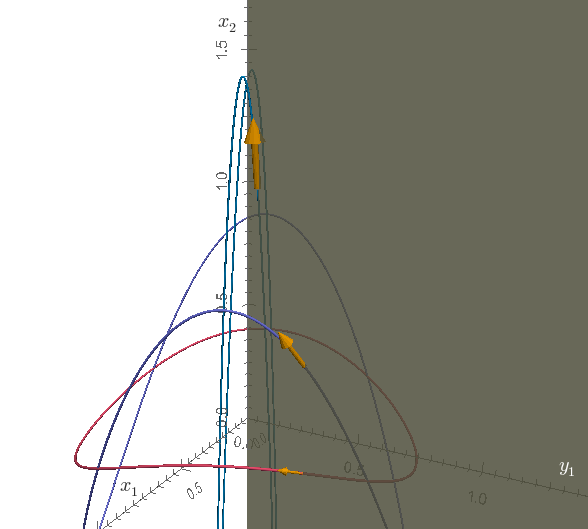
\includegraphics[width=0.65\textwidth]{BBmagicslicehd}
\caption{Fancy 3D visualization of the magic slice, group orbits and group tangents.}
\label{fig:BBmagicslicehd}
\end{figure}

\item[2013-11-17 Burak]
After realizing that I can do it, I wrote some scripts that converts solutions
to vtk data files that can be readable by Paraview, and plotted curves as 3D
objects. An example is \reffig{fig:BBeqvarnslice} where I drew the symmetry
equivariant and sliced flow on top of each other. I'm not sure if this may be
helpful in explaining the \mslices, but I think it's beautiful, so I'm blogging it.

My vtkscripts are here:
\\
\texttt{blog/burak/PorterKnobloch/paraview/vtkscripts/}

\begin{figure}%[H]
\centering
  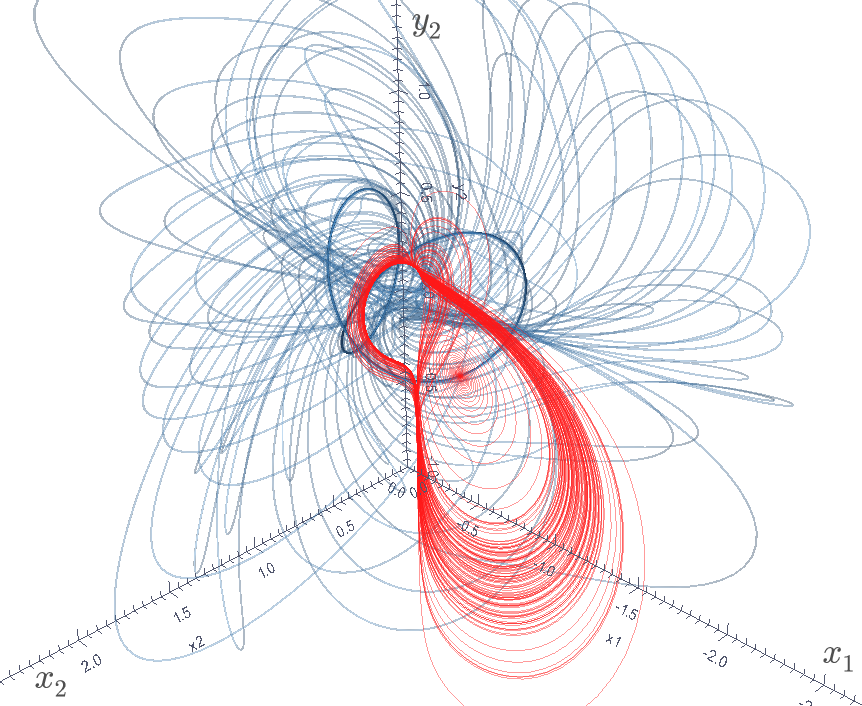
\includegraphics[width=0.65\textwidth]{BBeqvarnslice}
\caption{A chaotic trajectory and the \reqv\ \REQV{}{1} of
the full 4\dmn\ $\{x_1, y_1 ,x_2, y_2\}$ \statesp\ equivariant flow
projected on three coordinates
$\{x_1, ,x_2, y_2\}$, plotted together
with the symmetry-reduced flow
within the magic slice.}
\label{fig:BBeqvarnslice}
\end{figure}

\item[2013-11-18 Predrag] My reading of
\reffig{fig:BBmagicslicehd} is that Ruslan Davidchack, Evangelos Siminos
and Al Shapere are right. Unless I am missing some subtlety about the
invisible second dimension of the magic slice, it looks like we are
allowed to rotate it around the $x_2$ axis, and at all angles of that
rotation, all group orbits (as long as all Fourier coefficients are non-vanishing)
are sliced only once. In particular, if the slice group tangent vector is normal to
$y_1$, all group orbits intersect the (rotated) magic slice orthogonally.
If that is true, the simplest of all guesses at a slice might work, after all...
That would be good news.
What am I missing?

\item[2013-11-18 Burak] You are not missing anything. I went back and rechecked
my algebra and found a mistake (a division by zero), so it should be rotatable,
as geometry suggests. There is one point that I do not agree with Ruslan, I
remember him suggesting at some point that integration within the slice shouldn't
be used and one should always post process the data; I think that the opposite
is the best idea since we want to resolve the dynamics within the slice so
our integration steps must adapt to the velocity functions within the slice.
I still never managed to make numerics work on 1st mode slices other than
the magic slice, to which, right now I have no explanation to, but there should
be one.

\item[2013-11-18 Burak] Well I made them work, there were stupid mistakes before.
Now everything make sense and is less interesting. I suggest we discard the
magic slice and do the reduction onto $\slicep = (1,0,0,0)$. However, we
should carefully study its applicability to \KS\ and pipes, if it's not
applicable, then go back to the multiple chart atlas.

\item[2013-11-19 Burak] I made an argument before, saying that, in the \On{2}\
equivariant case, if the invariant polynomial $q$ vanishes in time, the flow
becomes effectively two dimensional ($w$ is determined by $u$ and $v$ through
the syzygy \refeq{eq:syzPK}). After discussing with Predrag yesterday and today
I decided to blog about it:

First of all, Danglemayr \rf{Dang86} never mentions $q$ or a syzygy. Since
we can produce the \On{2}\ symmetric system by setting $e_i \rightarrow 0$,
our invariant polynomials and the equations they satisfy should still be valid.

We can write down the velocity function for the invariant polynomials for the
$\On{2}$ case by setting $e_i \rightarrow 0$ in \refeq{PKinvEqs1} as

\bea% Triple checked ES 04-30-2012
  \dot{u} &=& 2\,\mu_1\,u+2\,a_1\,u^2+2\,b_1\,u\,v+c_1\,w %Double checked DB 04-29-2012
\continue
  \dot{v} &=& 2\,\mu_2\,v+2\,a_2\,u\,v+2\,b_2\,v^2+c_2\,w %Double checked DB 04-29-2012
\continue
  \dot{w} &=& (2\,\mu_1+\mu_2)\,w+(2a_1+a_2)\,u\,w+(2b_1+b_2)\,v\,w +\, 4c_1\,u\,v + 2c_2\,u^2
\label{O2invEqs1}\\
  \dot{q} &=& [2\mu_1+\mu_2+(2a_1+a_2)\,u+(2b_1+b_2)\,v\,]q
\,.
\nnu
\eea

Key observation here is that once we set $e_i \rightarrow 0$, $q$ gets decoupled
from the other equations and the final equation we got is actually linear in q,
with a time-varying real coefficient. For a first order linear differential
equation with real coefficients such the one we have here, only two things are
possible: it either diverges to infinity or converges to zero, depending on
the sign of coefficient being plus or minus. In our case, the coefficient
varies in time and it can change its sign depending on the parameters, which,
is indeed what I tried while looking for a chaotic attractor. However, after
experimenting on these parameters for a while, and having a second look at the
equations, I am thinking that $q$ either diverges or converges to 0.

As an experiment, I made a bifurcation diagram of q, similar to \reffig{fig:BBO2bifurcation}
by varying $a_1$, evaluating \refeq{O2invEqs1} for 1000 time units and recording
the last 100 values of q, and got \reffig{fig:BBO2qbifurcation}. As you can see most of the
time it converges to 0 and for the ones with values other than zero, I thought,
it could be converging slowly. To collect more evidence, I integrated \refeq{O2invEqs1} with
parameters \refeq{eq:parsO2a1only} setting $a_1 = 0.452121212121$ the $a_1$
value that corresponds to the largest peek in the bifurcation diagram \reffig{fig:BBO2qbifurcation}
and plotted $q$ versus time \reffig{fig:BBO2qt}. As you can see from the figure,
I proved myself wrong. In this case, $q$ oscillates regularly as the orbit is a
\rpo , but doesn't converge to anything.

For now, this discussion is inconclusive, however, I still think that we can
come up with an argument related to linear being of $\dot{q}$ and the dimensionality
of the system in the invariant polynomial basis to state that observing chaos
in the \On{2}\ normal forms that we are dealing here is impossible.

\begin{figure}%[ht]
  \begin{center}
  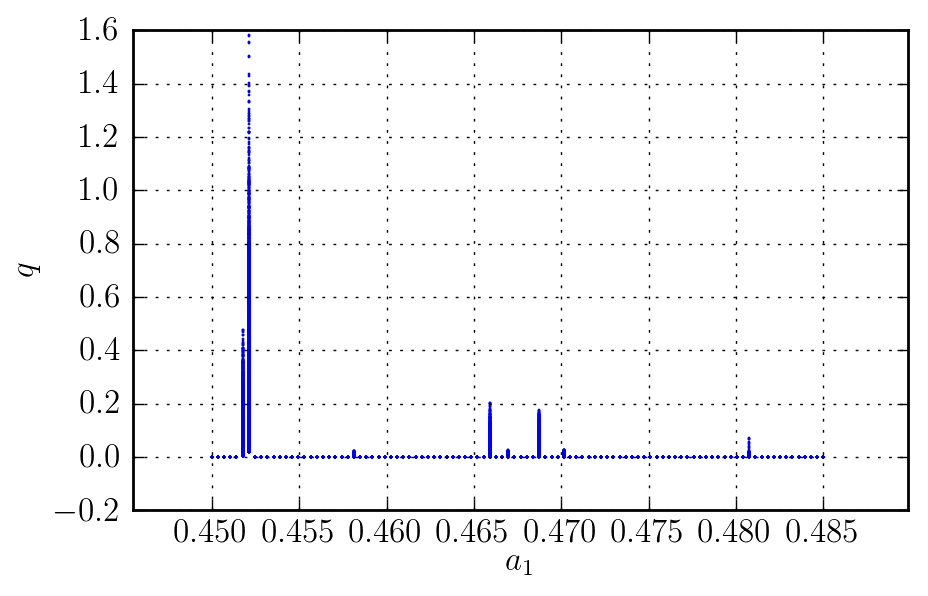
\includegraphics[width=0.8\textwidth]{BBO2qbifurcation}
  \end{center}
  \caption{
Bifurcation diagram for q in \On{2}\ invariant case obtained by integrating
\refeq{O2invEqs1} for 1000 time steps and keeping the last 100 of them with parameters \refeq{eq:parsO2a1only},
$a_1$ varying.
    }
  \label{fig:BBO2qbifurcation}
\end{figure}

\begin{figure}%[ht]
  \begin{center}
  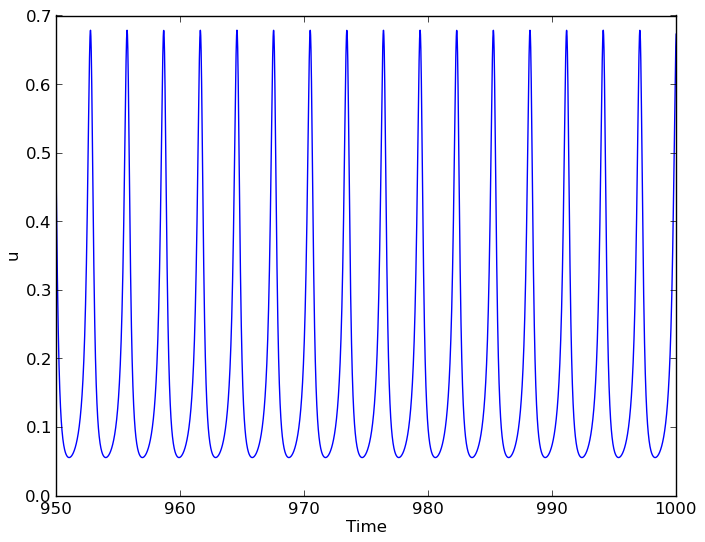
\includegraphics[width=0.8\textwidth]{BBO2qt}
  \end{center}
  \caption{
Invariant polynomial $q$ versus time, obtained by integrating \refeq{O2invEqs1},
using parameters \refeq{eq:parsO2a1only} with $a_1 = 0.452121212121$.
    }
  \label{fig:BBO2qt}
\end{figure}

\item[2013-12-08 Burak] Found \rpo s and their binary itineraries, blogging
a preliminary result in \reftab{tab:symbdyn}. While \reftab{tab:symbdyn} has 50 \rpo s,
some of them computed multiple times, so the code needs some improvment.
Also looking at these numbers, accuracy that I could get was around 4 decimal
places, which is not so great. I used the build in Newton solver \texttt{fsolve}
from \HREF{http://www.scipy.org/}{SciPy} , which is an implementation of
\texttt{hybrd} and \texttt{hybrdj} functions from \HREF{http://www.netlib.org/minpack/}
{MINPACK Fortran library} requiring relative accuracy of $10^{-12}$ between iterations.

After a little more investigation, I found out that the \rpo s with higher periods
are not accurate at all. I developed the algorithm to search for \rpo s on the
Poincar\'e section this weekend, however, it ended up being less successful then
looking at the reduced \statesp\ which is what I did last week. I'm blogging
the figure of two \rpo s here: \reffig{fig:BBrpo}. By going back to my
previous algorithm, I probably will add a third one here.

Searching for cycles had been more challenging than I expected and now I'm really
short on time. I am switching to the Dynamics Days poster right now.

\begin{figure}%[ht]
  \begin{center}
  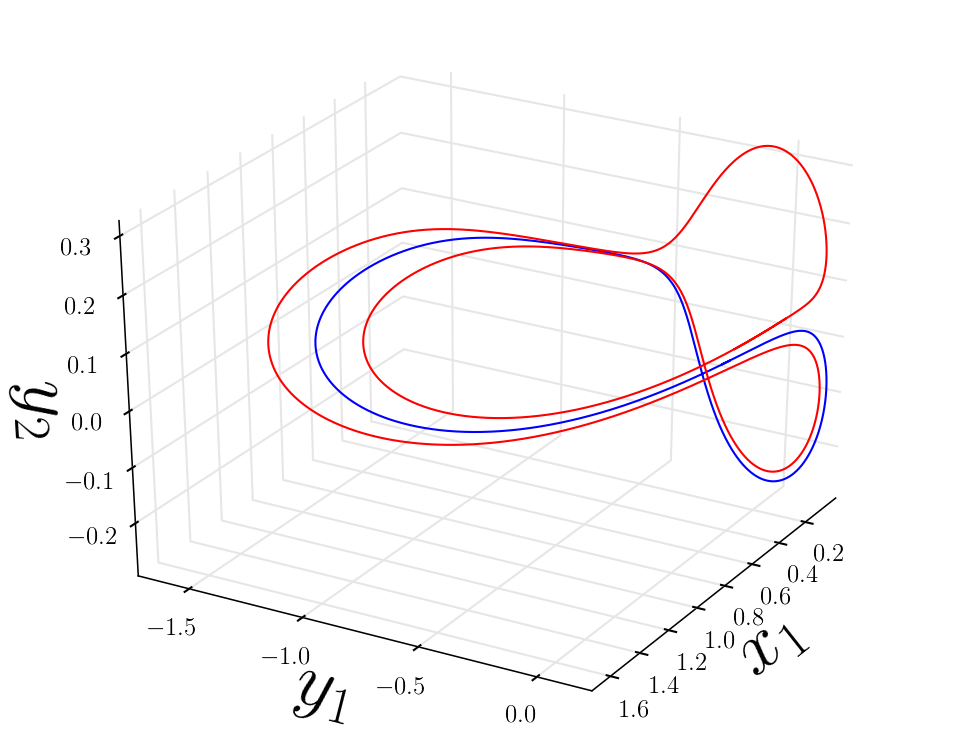
\includegraphics[width=0.8\textwidth]{BBrpo}
  \end{center}
  \caption{
	\Rpo s \cycle{1} and \cycle{01} for  the \twoMode\ system.
    See also \reffig{fig:2modeRPOs}.
    }
  \label{fig:BBrpo}
\end{figure}

\begin{table}
	\begin{tabular}{c|c}
	Itinerary & $(x_{1,RPO}, y_{1,RPO}, x_{2,RPO}, y_{2,RPO})$ \\ 
	\hline
	1  & (0.4525310, 0.0000000, 0.0491730, 0.0323220) \\ 
 	\hline
	01  & (0.4516980, 0.0000000, 0.0202880, 0.0389600) \\ 
 	\hline
	10  & (0.4532780, 0.0000000, 0.0750390, 0.0254810) \\ 
 	\hline
	011  & (0.4501950, 0.0000000, -0.0317750, 0.0497160) \\ 
 	\hline
	011  & (0.4502030, 0.0000000, -0.0315070, 0.0498950) \\ 
 	\hline
	010  & (0.4519660, 0.0000000, 0.0295760, 0.0379080) \\ 
 	\hline
	111  & (0.4524410, 0.0000000, 0.0460270, 0.0312930) \\ 
 	\hline
	100  & (0.4551600, 0.0000000, 0.1402620, 0.0056040) \\ 
 	\hline
	101  & (0.4550160, 0.0000000, 0.1352850, 0.0066550) \\ 
 	\hline
	0101  & (0.4515050, 0.0000000, 0.0135930, 0.0402150) \\ 
 	\hline
	1101  & (0.4521150, 0.0000000, 0.0347420, 0.0369650) \\ 
 	\hline
	1110  & (0.4529440, 0.0000000, 0.0634840, 0.0302250) \\ 
 	\hline
	1011  & (0.4536200, 0.0000000, 0.0868880, 0.0226260) \\ 
 	\hline
	11111  & (0.4525310, 0.0000000, 0.0491590, 0.0323140) \\ 
 	\hline
	01111  & (0.4506150, 0.0000000, -0.0172370, 0.0462820) \\ 
 	\hline
	01011  & (0.4519510, 0.0000000, 0.0290460, 0.0374940) \\ 
 	\hline
	11011  & (0.4519890, 0.0000000, 0.0303710, 0.0373340) \\ 
 	\hline
	11010  & (0.4522340, 0.0000000, 0.0388630, 0.0353260) \\ 
 	\hline
	11111  & (0.4525050, 0.0000000, 0.0482420, 0.0325480) \\ 
 	\hline
	10101  & (0.4530350, 0.0000000, 0.0666150, 0.0278020) \\ 
 	\hline
	10101  & (0.4530290, 0.0000000, 0.0663980, 0.0283200) \\ 
 	\hline
	11011  & (0.4545930, 0.0000000, 0.1206200, 0.0504560) \\ 
 	\hline
	10110  & (0.4546190, 0.0000000, 0.1215170, 0.0108250) \\ 
 	\hline
	111111  & (0.4523800, 0.0000000, 0.0439200, 0.0294930) \\ 
 	\hline
	011101  & (0.4513060, 0.0000000, 0.0067200, 0.0431280) \\ 
 	\hline
	010110  & (0.4518470, 0.0000000, 0.0254650, 0.0374470) \\ 
 	\hline
	110101  & (0.4521470, 0.0000000, 0.0358570, 0.0355210) \\ 
 	\hline
	111101  & (0.4522560, 0.0000000, 0.0396370, 0.0346230) \\ 
 	\hline
	111101  & (0.4523580, 0.0000000, 0.0431560, 0.0351780) \\ 
 	\hline
	111111  & (0.4525310, 0.0000000, 0.0491730, 0.0323220) \\ 
 	\hline
	111111  & (0.4528270, 0.0000000, 0.0594120, 0.0371410) \\ 
 	\hline
	111111  & (0.4524840, 0.0000000, 0.0475170, 0.0327290) \\ 
 	\hline
	101010  & (0.4531900, 0.0000000, 0.0720050, 0.0261900) \\ 
 	\hline
	111111  & (0.4525310, 0.0000000, 0.0491730, 0.0323220) \\ 
 	\hline
	101111  & (0.4538490, 0.0000000, 0.0948170, 0.0214900) \\ 
 	\hline
	0110101  & (0.4504000, 0.0000000, -0.0246730, 0.0487990) \\ 
 	\hline
	0110101  & (0.4503810, 0.0000000, -0.0253450, 0.0473590) \\ 
 	\hline
	0111101  & (0.4508060, 0.0000000, -0.0106260, 0.0464390) \\ 
 	\hline
	0111101  & (0.4508250, 0.0000000, -0.0099580, 0.0465640) \\ 
 	\hline
	0011111  & (0.4509220, 0.0000000, -0.0065940, 0.0722500) \\ 
 	\hline
	0111011  & (0.4515410, 0.0000000, 0.0148390, 0.0417900) \\ 
 	\hline
	0101111  & (0.4519500, 0.0000000, 0.0290300, 0.0372790) \\ 
 	\hline
	1101111  & (0.4520600, 0.0000000, 0.0328350, 0.0385940) \\ 
 	\hline
	1101010  & (0.4521500, 0.0000000, 0.0359670, 0.0371310) \\ 
 	\hline
	1101111  & (0.4520040, 0.0000000, 0.0309010, 0.0393920) \\ 
 	\hline
	1101010  & (0.4521420, 0.0000000, 0.0356680, 0.0364640) \\ 
 	\hline
	1101010  & (0.4521460, 0.0000000, 0.0358010, 0.0367990) \\ 
 	\hline
	1111111  & (0.4524990, 0.0000000, 0.0480570, 0.0325970) \\ 
 	\hline
	1111010  & (0.4523470, 0.0000000, 0.0427940, 0.0336690) \\ 
 	\hline
	1111111  & (0.4525200, 0.0000000, 0.0487720, 0.0328350) \\ 
 	\end{tabular}
	\caption{Symbolic dynamics of \twoMode\ system.}
	\label{tab:symbdyn}
\end{table}

\item[2013-12-10 Predrag] You have to get a good multiple shooting
or variational \rpo\ Newton
routine running, you'll need it later. Here we expect all periodic
points and cycle stabilities to machine precision.

You need to list only one periodic point per cycle, lexically
ordered, as in ChaosBook
\HREF{http://www.streamsound.dk/book1/chaos/chaos.html\#323/z}
{Table 15.1}. I have removed some of the repeats and extra
cycle points. Current accuracy is sub par.

\cycle{101010} = \cycle{10}$^3$ is the third repeat of \cycle{10}.

We also need a short list of periods, phases, Floquet multipliers
and Floquet exponents for these cycles. I'll try to recycle some
old table, but - curiously enough - neither Siminos nor Davidchack nor
Froelich seem to have created such a table...


There will be pruning, as in
\HREF{http://www.streamsound.dk/book1/chaos/chaos.html\#249/z}
{11.5 Kneading theory} - should mention it. It is the kneading invariant
obtained by the forward iteration of the critical (the highest) point of
the return map.

\item[2014-01-19 Burak to Predrag] I came to the point of applying the multiple
shooting method to the Rossler system and before coding, I finished reading
\HREF{http://chaosbook.org/version14/paper.shtml\#cycles}{Chapter 13 - Fixed points, and how to get them}
and got confused. Last time when we talked at your office, you told me that
when I set up a Newton search for a relative periodic orbit, I should add the
symmetry parameters and time to the list of variables that I am looking for
and run the search in the full \statesp . However, in 13.4, in summary, you
say that when one looks for a particular orbit with a continuous symmetry, such
as a periodic orbit symmetric under time translations, one has a marginal
Floquet multiplier, hence  $(1 - J)$ which appears in the Newton set up becomes
non-invertible. For this reason, one should always applies a constraint, such
as a Poincar\'e section to the Newton solver to make it convergent. This was
my initial idea and I looked for the periodic orbits within the slice and the
Poincare section in the \twoMode\ system, then we decided that I should apply
multiple shooting method. Did you have any particular reason for looking for the
\rpo s in the full \statesp ?

\item[2014-01-20 Burak] Here (\reffig{fig:BBrosslerPO}) are two long periodic
orbits of Rossler system that I found by multiple shooting method on the Poincare
section. I'm not committing the code yet since parts of it is assigned as a
homework problem for the ChaosBook course. Tomorrow, I will start adapting
the algorithm to \twoMode\ system to find the \rpo s with an acceptable
precision.

\begin{figure}%[H]
\centering
 (a) 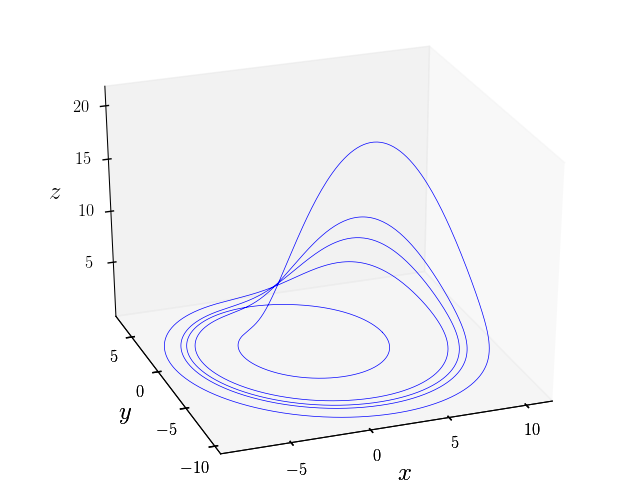
\includegraphics[width=0.35\textwidth]{BBrossler01111}
 (b) 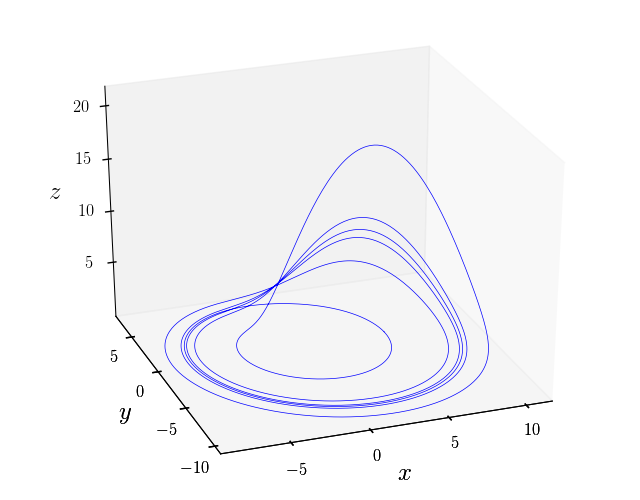
\includegraphics[width=0.35\textwidth]{BBrossler011111}
\caption{(a) Periodic orbit 01111 of Rossler system. (b) Periodic orbit 011111 of Rossler system.}
\label{fig:BBrosslerPO}
\end{figure}

\renewcommand{\zeit}{\ensuremath{\tau}}  %time variable
\item[2014-01-31 Burak, 2014-02-03 Predrag]            \toCB
\\{\bf Multiple shooting method for search for the \rpo s:}
Let us assume that we have a set of good guesses
for a set of \statesp\ points,
flight times and
$1D$ symmetry group parameter increments
$\{\ssp_i^{(0)}\,,\,\zeit_i^{(0)}\,,\,\gSpace_i^{(0)}\}$
such that the points
$\{\ssp_i^{(0)}\}$
lie close to the \rpo\ $p$,
\beq
	\ssp_{i+1}^{(0)} \approx \LieEl (\gSpace_i^{(0)}) \flow{{\zeit_i^{(0)}}}{\ssp_i^{(0)}}
    \quad  \mbox{cyclic in $i = 1, ..., n$}
\,.
\eeq
Here the period and the shift of the \rpo\ $p$ are
$\period{p} \approx \sum \zeit_i\,,$
$\gSpace_p \approx \sum \gSpace_i \,.$
We want to determine
$(\Delta\ssp_i\,,\,\Delta\zeit_i\,,\,\Delta\gSpace_i)$
corresponding to the exact \rpo,
\beq
	\ssp_{i+1} + \Delta \ssp_{i+1} = \LieEl (\gSpace_i + \Delta \gSpace_i)
		\flow{\zeit_i + \Delta \zeit_i}{\ssp_i + \Delta \ssp_i}
		\quad  \mbox{cyclic in } i = 1, ..., n
\,.
\eeq
To linear order in
\[
(\Delta\ssp_i^{(m+1)}\,,\, \Delta\zeit_i^{(m+1)}\,,\,\Delta\gSpace_i^{(m+1)})
=
(\ssp_i^{(m+1)}-\ssp_i^{(m)}\,,\,
 \zeit_i^{(m+1)}-\zeit_i^{(m)}\,,\,
 \gSpace_i^{(m+1)}-\gSpace_i^{(m)})
\]
the improved Newton guess
$
(\ssp_i^{(m+1)}\,,\,\zeit_i^{(m+1)}\,,\,\gSpace_i^{(m+1)} )
$
is obtained by minimizing the effect of perturbations along
the spatial, time and phase directions,
    \PC{2014-02-02 I have changed Burak's \refeq{PCnetwonStep} by
    $\Lg \flow{\zeit_i}{\ssp_i}
        \to
    \Lg \LieEl (\gSpace_i)\flow{\zeit_i}{\ssp_i}$.
    The rest of the formulas need to be changed accordingly.}
    \PC{2014-02-02 to Burak: please write up the detailed
    derivation, with what $O(\Delta^2)$'s are dropped
    as a problem / solution set for \texttt{cycles.tex}.}
\beq
	\ssp_{i+1}^{'} - \LieEl_{i+1} \flow{{\zeit_i}}{\ssp_i}
= \LieEl_{i+1}\left(
  \groupTan_{i+1} \Delta \gSpace_i
+ \vel_{i+1} \Delta \zeit_i
+ \jMps_{i+1} \Delta \ssp_i
    \right)
\,,
\ee{PCnetwonStep}
where, for brevity,
$\ssp_{i}^{(m+1)} = \ssp_{i}^{(m)} + \Delta \ssp_{i}^{(m)}
   = \ssp_{i}^{'}$,
$\ssp_{i}^{(m)} = \ssp_{i}$,
$\LieEl (\gSpace_i) = \LieEl_{i+1}$,
$\vel (\ssp_{i}) = \vel_i$,
$\jMps^{\zeit_i}(\ssp_i) = \jMps_{i+1}$,
$\groupTan(\ssp_{i}) = \Lg \ssp_{i} = \groupTan_i$,
\etc.
For sufficiently good initial guesses,
the improved values converge under Newton iterations to
the exact values
$(\Delta\ssp_i\,,\,\Delta\zeit_i\,,\,\Delta\gSpace_i)$
=$(\Delta\ssp_i^{(\infty)}\,,\,\Delta\zeit_i^{(\infty)}\,,\,\Delta\gSpace_i^{(\infty)})$
at a super-exponential rate.
    \PC{2014-02-02 I am often running into the situation that the linear
    operators are better marked by the final rather than by the initial
    points of trajectory segments, as in $\jMps^{\zeit_i}(\ssp_i) =
    \jMps_{i+1}$. Implementing this requires a huge rewrite of the
    ChaosBook}
%
%Regrouping terms we get a form that we can turn to a matrix equation:
%\beq
%	 \LieEl (\gSpace_i) \jMps^{\zeit_i}(\ssp_i) \Delta \ssp_i
%	+ \LieEl (\gSpace_i) \vel (\flow{\zeit_i}{\ssp_i}) \Delta \zeit_i
%	+\Lg \flow{\zeit_i}{\ssp_i} \Delta \gSpace_i
%	- \Delta \ssp_{i+1}
%	= \ssp_{i+1} - \LieEl (\gSpace_i) \flow{\zeit_i}{\ssp_i}
%\eeq
In order to deal with the marginal multipliers along the time and group
orbit directions, one needs to apply a pair of constraints, which
eliminate variations along the marginal directions on the \rpo s\ $2D$
torus (see \reffig{fig:BBO2RpoSspComovSlice}). As our guesses
$\{\ssp_i^{(m)}\}$ are
computed in the global slice \reffig{fig:BBpsecthd} and Poincar\'e
section \reffig{fig:psectandretmap}\,(a),
%Parameters: \refeq{eq:parsO2a1only} with $a_1 = 0.45$.
and read off the (nearly)
unimodal return map \reffig{fig:psectandretmap}\,(b), one can
impose the corresponding global slice and section constraints
\refeq{eq:firstmodetemplate} and \refeq{eq:nhat0GS-1},
\beq
[write the global constraints here]
\,,
\ee{RPOConstrsGlobal}
for each return map cycle point $\ssp_i$ in \reffig{fig:psectandretmap}\,(b),
compute the first return time and phase shift
$(\ssp_i^{(m)}\,,\,\zeit_i^{(m)}\,,\,\gSpace_i^{(m)} )$,
and then restart with $\ssp_{i+1}$ in \reffig{fig:psectandretmap}\,(b).

However, imposition of the global slice condition induces high
velocities along the phase reconstruction coordinate $\dot{\gSpace}(\zeit)$
close to the {\chartBord}. These high $\dot{\gSpace}(\zeit)$
are artifacts of the symmetry reduction methods, they are not present in
the full \statesp\ flow.
For that reason local transversality constraints -
a local Poincar\'e section orthogonal to the flow, and a local slice
orthogonal to the group orbit at each point along the orbit,
\beq
   \vel_i \cdot \Delta x_i = 0
\,,\qquad
   \groupTan_{i} \cdot \Delta x_i = 0
\,,
\ee{RPOConstrsLocal}
are natural and numerically preferable; in the limit of infinitely many
infinitesimal time steps, the solutions that they yield are the \rpo s in
the {\comovframe} transformed equations \refeq{transvFlow}, see
\reffig{fig:BBO2RpoSspComovSlice}\,(b), with the {\comovframe}
$\gSpace_{p}^{cm}$. This $\gSpace_{p}^{cm}$ might be the so much bandied
around `geometrical phase.'. As the {\mconn} is not a symmetry-reduction
method, the trajectory explores ergodically the same invariant torus, but
with a different shift per period. Once the \rpo\ is computed, its shift
$\gSpace_p$ in the `lab frame' can be computed by imposing the fixed
slice condition \refeq{RPOConstrsGlobal} on any cycle point.

We can rewrite everything as one matrix equation:
\beq \label{eq:multishootmatrix}
	{\bf A} \Delta = E,
\eeq
where,
\beq \label{eq:AforNewton}
	{\bf A} = \\
	\begin{pmatrix}
	  \LieEl_{2} \jMps_{2} &
	  \LieEl_{2} \vel_2 &
	  \Lg \LieEl_{2} \flow{\zeit_1}{\ssp_1}  &
	  - \matId & 0 & 0 & 0 & \cdots & 0 \\
	  \vel_1 & 0 & 0 & 0 & 0 & 0 & 0 & \cdots & 0 \\
	  \sliceTan{} & 0 & 0 & 0 & 0 & 0 & 0 & \cdots & 0 \\
	  0 & 0 & 0 &
	  \LieEl_{3} \jMps_{3} &
	  \LieEl_{3} \vel_3 &
	  \Lg \LieEl_{3} \flow{\zeit_2}{\ssp_2}   &
	  - \matId & \cdots & 0 \\
	  0 & 0 & 0 & \vel_2 & 0 & 0 & 0 & \cdots & 0 \\
	  0 & 0 & 0 & \sliceTan{} & 0 & 0 & 0 & \cdots & 0 \\
	  \vdots & \vdots & \vdots & \vdots & \vdots & \vdots & \vdots & \ddots & \vdots \\
	  - \matId & 0 & \cdots & 0 & 0 & 0 &
	  \LieEl_{1} \jMps_{1} &
	  \LieEl_{1} \vel_1 &
	   \Lg \LieEl_{1} \flow{\zeit_1}{\ssp_1}   \\
	  0 & 0 & \cdots & 0 & 0 & 0 & \vel_n & 0 & 0 \\
	  0 & 0 & \cdots & 0 & 0 & 0 & \sliceTan{} & 0 & 0
	 \end{pmatrix}	
\eeq
\beq \label{eq:DeltaandE}
	\Delta =
	 \begin{pmatrix}
	  \Delta \ssp_1 \\
	  \Delta \zeit_1 	\\
	  \Delta \gSpace_1 \\
	  \Delta \ssp_2 \\
	  \Delta \zeit_2 	\\
	  \Delta \gSpace_2 \\
	  \vdots \\
	  \Delta \ssp_n \\
	  \Delta \zeit_n 	\\
	  \Delta \gSpace_n \\
	 \end{pmatrix}  	
	 \ \mbox{and} \
	 E =
	 \begin{pmatrix}
	  \ssp_{2} - \LieEl_2 \flow{\zeit_1}{\ssp_1} \\
	   0 	\\
	   0 	\\
	  \ssp_{3} - \LieEl_3 \flow{\zeit_2}{\ssp_2} \\
	  0 	\\
	  0 \\
	  \vdots \\
	  \ssp_{1} - \LieEl_1 \flow{\zeit_n}{\ssp_n} \\
	  0 	\\
	  0 	\\
	 \end{pmatrix}
\eeq
We than solve \refeq{eq:multishootmatrix} for $\Delta$ and update our initial
guess by adding the vector of the computed $\Delta$ values, and iterate.

I applied this algorithm to the \rpo\ candidates that I found from the return
map to get the \rpo s precisely, however, orbits, other than \cycle{1} did not
converge.

I also added an adaptive stepping algorithm which basically reduces the
step length if a Newton step increases the error, after adding this, it
search started to converge a non-zero minimum value. I plotted the
element of $E$ with largest absolute value which, for \cycle{01} looks
like \reffig{fig:errorrposearch}.

One thing, that I clearly see by looking at the numbers is that, while the
constraint $\sliceTan{} \cdot \Delta x_i$  keeps $(\Delta x_i)_2 = 0$, since,
$\sliceTan{} = (0,1,0,0)$, maximum error in $E$ appears to be in the second
element of each $\ssp_{i+1} - \LieEl (\gSpace_i) \flow{\zeit_i}{\ssp_i}$. This can
either due to $\zeit_i$ or $\gSpace_i$ variations, since $(\Delta x_i)$ obeys the
constraint and keeps $y_1$ component of the $\ssp_i = 0$.

%%%%%%%%%%%%%%%%%%%%%%%%%%%%%%%%%%%%%%%%%%%%%
\SFIG{errorrposearch}
{}{
Error vs Newton search steps for \rpo\ \cycle{01} of \twoMode\ system.
}{fig:errorrposearch}
%%%%%%%%%%%%%%%%%%%%%%%%%%%%%%%%%%%%%%%%%%%%%

There must be something I am missing, however, I could not find it yet. Any
suggestions? Maybe a restriction on $\zeit_i$'s or $\gSpace_i$'s?

This derivation is based on eq.~(13.11) of
\HREF{http://www.streamsound.dk/book1/chaos/chaos.html\#294/z}
{Fixed points and how to get them}.
%\item[2014-02-02 Predrag] moved to dasbuch/blog/chapter/cycles.cycles
% and while working on it, I realized a
%sign error in (13.11), there should be a $-$ sign before $\vel (x)$ in the
%first row, you can see this by comparing (13.9) and (13.11), in (13.9), after
%Taylor expansion, Jacobian and velocity terms have the same sign, as they
%should, but the velocity term in the matrix of (13.11) misses its minus sign.

\renewcommand{\zeit}{\ensuremath{t}}  %time variable
\item[2014-02-02 Predrag] An idea of how to represent the \twoMode\
\statesp. The splaying of the strange attractor close to the {\sliceBord}
in \reffig{fig:Set1}\,(d) is an artifact of the Fourier modes
representation. Think of a straight line, constant velocity trajectory in
Cartesian $(x_1(\zeit),x_2(\zeit))$ coordinates passing close to the
origin (our {\sliceBord}). In polar coordinates $ {z}_1 = |u|^{1/2}
e^{\ii\theta_1}$, $ {z}_2 = |v|^{1/2} e^{\ii\theta_2}$, $|u|(\zeit) \to
0_+$, and $\dot{\theta}(\zeit)$ whips through,
$\dot{\theta}(\zeit)$ making a fast jump by
$\pm\pi$, see \cLf\ \reffig{fig:singpass}. So we should really chose more
sensible coordinates which rescale $\dot{\gSpace}$ in such a way that
when the trajectory passes by the singularity as a straight line, the new
velocity is nearly constant vector as the trajectory passes the
singularity.

%%%%%%%%%%%%%%%%%%%%%%%%%%%%%%%%%%%%%%%%%%%%%%%%%%%%%%
\SFIG{singpass1}
{}{The blue trajectory passes through the {\sliceBord} of \cLf. Notice
how there is the gap in the trajectory, this corresponds to the jump
cause by passing through the singularity. The red trajectory has initial
point differing from the blue's by $(0,0,0.1,0,0)$, so it does not pass
through a singularity. The green trajectory is the group orbit of
$x_{sing}$ between the two $\gSpace$ that rotate $v(x_{sing})$ in the
slice. As expected, the red trajectory begins near the blue trajectory,
closely follows the green trajectory after the singularity point, reaches
the other side of the blue trajectory and begins to follow it again. Read
Sect.~2.6~{\em Slice singularities} in \texttt{siminos/froehlich/blog.pdf}.
}{fig:singpass}
%%%%%%%%%%%%%%%%%%%%%%%%%%%%%%%%%%%%%%%%%%%%%%%%%%%%%%

\item[2014-02-02 Predrag] Another idea of how to visualize the \twoMode\
states. We are toying with the \twoMode\ system as a model for truncations
of $1D$ PDEs such as \KS. For those the natural visualization is in the configuration
space, \ie, as a periodic function
$u(x,t)=u(x+2\pi,t)$ on the  domain $x \in [0,2\pi]$.
You can think of $({z}_1,{z}_2)$ as the coefficients in the $k=\{1,2\}$ truncation
of the Fourier expansion
\beq
  u(x,t)=\sum_{k=-\infty}^{+\infty} z_k (t) e^{ i k x /2\pi }
\,.
\ee{eq:BBtwoModeExp}
How about doing the inverse Fourier transform, and plotting color coded
amplitude $u(x,\zeit)$ in the $[x,\zeit]$ plane, as we do (for example)
in \refref{SCD07}
(\HREF{http://www.cns.gatech.edu/~predrag/papers/preprints.html\#SCD07}{click
here}). Chaotic dynamics is competition between 1-wiggle and 2-wiggle
solutions, that might be more obvious in the configuration space. \Reqva\
and \rpo s will drift with different {\phaseVels}. One can perhaps study
energy, dissipation rate, \etc? In other words, motivate the model by
the physical problems we are really interested in.

\item[2014-02-02 Predrag] I started rewriting the
multiple shooting method for search for the \rpo s, with intention of
including it into ChaosBook. As an example? exercise? in an appendix? -
in any case have to include the calculation for a \reqv,
possibly in the Lagrange multiplier formulation, if that is easier to
understand...

I stopped, however, until Burak edits the formulas.

\item[2014-02-03 Predrag] You
\HREF{http://www.streamsound.dk/book1/chaos/chaos.html\#290/z} {always
want to plot} $\log_{10}$(error) in \reffig{fig:errorrposearch}, to
verify the you are getting the quadratic super-exponential convergence
expected of Newton. What happened to odd iterations?

\item[2014-02-03 Predrag] What bugs me about Newton is that one must pick
a particular norm in \refeq{RPOConstrsLocal}; that is very
explicit in the Lagrangian {\costFct} formulation of the boyscout version
of ChaosBook. So in applying this to \KS\ you should try different
Sobolev norms. Would be grand if there were a norm-free iteration
method...

\item[2014-02-03 Burak] I think choosing
the global slice for every point is a better idea for our approach, since
our guesses are from that particular slice and if we force them to move
in their local slice, our initial guesses may be not as good as they were before.
\\
{\bf [2014-02-03 Predrag]} Do not worry, the
errors will drop like a ton of rocks,
with no need to use short time steps close to close to the {\chartBord}.

\item[2014-02-03 Burak]
% After adding the missing term, mutlishoot \rpo\
% searches started to become successful.
Here are
four \rpo s in the \slice\ hyperplane: \refFig{fig:2modeRPOs}.

\begin{figure}%[H]
\centering
 ~~~~~~\cycle{01} 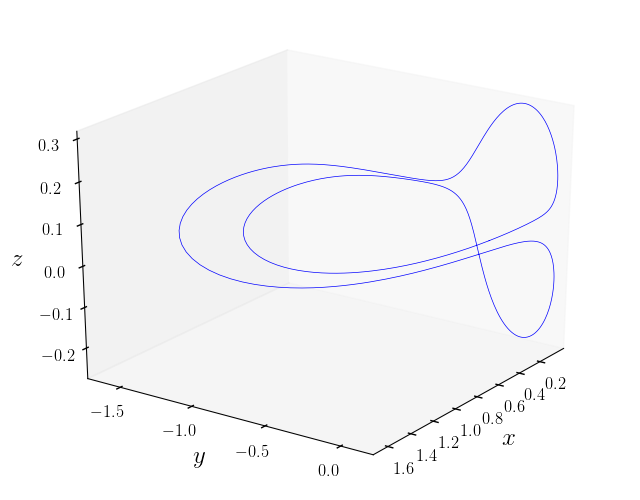
\includegraphics[width=0.3\textwidth]{BBPK01}
 ~~\cycle{01101} 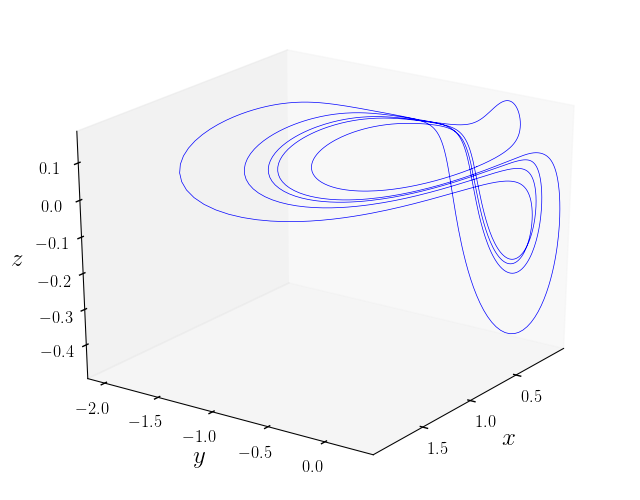
\includegraphics[width=0.3\textwidth]{BBPK01101}
 \\
 \cycle{011101} 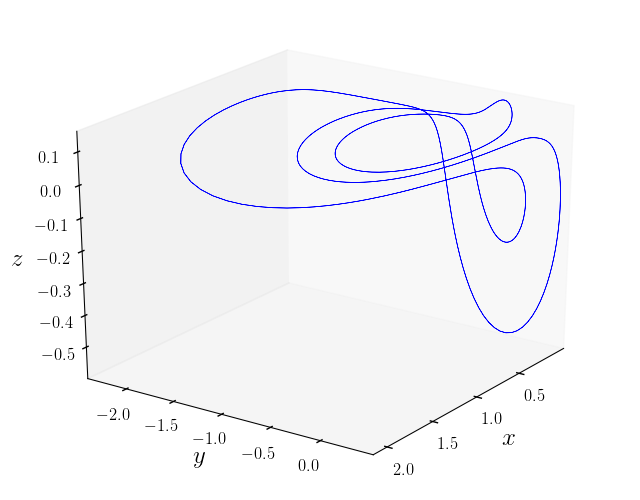
\includegraphics[width=0.3\textwidth]{BBPK011101}
 \cycle{011111} 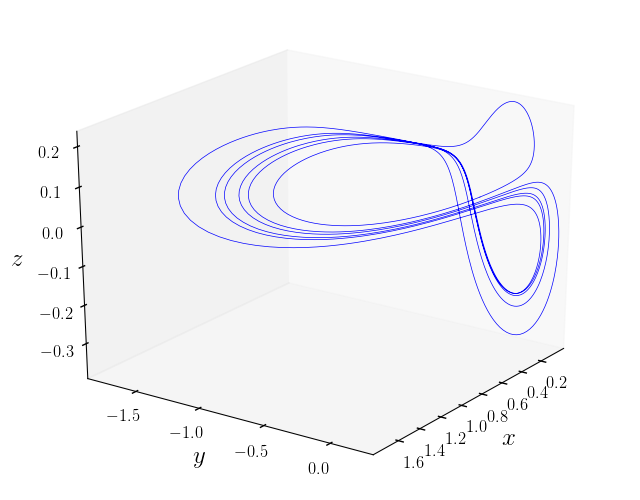
\includegraphics[width=0.3\textwidth]{BBPK011111}
\caption{
Several \rpo s of \twoMode\ system  plotted in the \slice\ hyperplane.
Cycle \cycle{011111} exhibits accumulation toward \cycle{1} for
long sequences of consecutive 1's.
See also \reffig{fig:BBrpo1-01}.
}
\label{fig:2modeRPOs}
\end{figure}

\item[2014-02-03 Predrag]
You have to explain and plot the critical point (top of the knifedge)
in \reffig{fig:psectandretmap}\,(b). It is worked out for the Lorenz in
ChaosBook.

\begin{figure}%[H]
\centering
   \begin{tabular}{c c c c}
   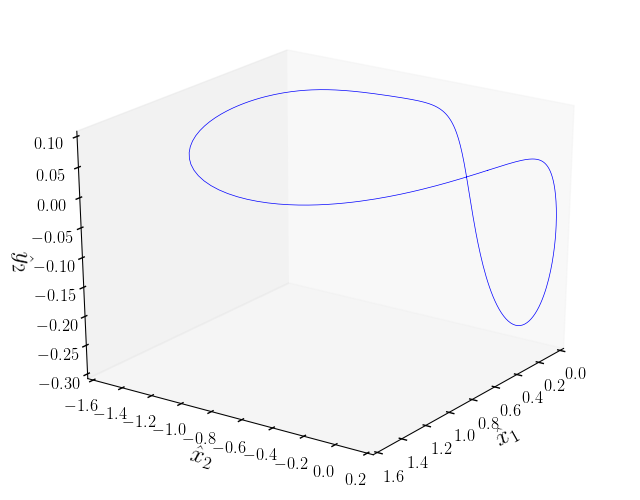
\includegraphics[width=0.2\textwidth]{PK1slice}
 & 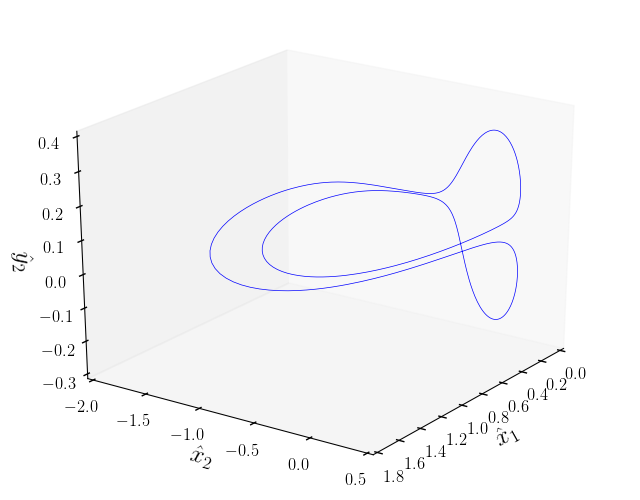
\includegraphics[width=0.2\textwidth]{PK01slice}
 & 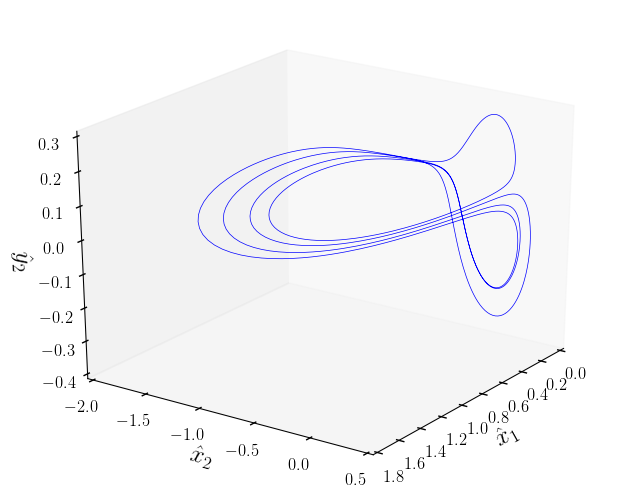
\includegraphics[width=0.2\textwidth]{PK0111slice}
 & 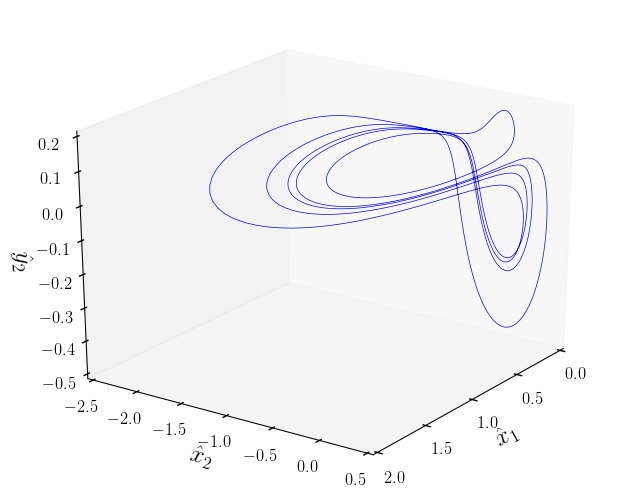
\includegraphics[width=0.2\textwidth]{PK01101slice} \\
   \includegraphics[width=0.2\textwidth]{PK1conf}
 & \includegraphics[width=0.2\textwidth]{PK01conf}
 & \includegraphics[width=0.2\textwidth]{PK0111conf}
 & \includegraphics[width=0.2\textwidth]{PK01101conf}\\
 \cycle{1} & \cycle{01} & \cycle{0111} & \cycle{011101}
   \end{tabular}

\caption{
Several \rpo s of \twoMode\ system  plotted in the slice (top) and the configuration
space (bottom).
}
\label{fig:2modeRPOswconf}
\end{figure}


\item[2014-02-07 Burak]
\Rpo s, their symbolic dynamics and periods are listed in
\reftab{tab:twomoderpos}.

\begin{table}
	\begin{tabular}{c|c|c}
	Itinerary & $(x_{p,1}, y_{p,1}, x_{p,2}, y_{p,2})$ & Period \\
	\hline
	1 & (0.4525719,   0.0, 0.0509257, 0.0335428) & 3.6415120 \\
 	\hline
	01 & (0.4517771,   0.0, 0.0202026, 0.0405222) & 7.3459412 \\
 	\hline
	0111 & (0.4514665,   0.0, 0.0108291, 0.0424373) & 14.6795175 \\
 	\hline
	01101 & (0.4503967,   0.0, -0.0170958, 0.0476009) & 18.3874094 \\
 	\hline
	01111 & (0.4505384,   0.0, -0.0171185, 0.0475980) & 18.3874094 \\
 	\hline
	011111 & (0.4512323,   0.0, 0.0037677, 0.0438172) & 21.9923439 \\
 	\hline
	011101 & (0.4575102,   0.0, -0.0327127, 0.0497776) & 22.1591782 \\
 	\end{tabular}
	\caption{
The shortest \rpo s of the \twomode\ system.
Parameter values \reftab{tab:pars}\,(a).
    }
	\label{tab:twomoderpos}
\end{table}


\item[2014-02-07 Burak] We can define a new time variable as $d\tau = x_1 dt$
and rewrite \refeq{eq:so2reduced} for the first mode slice ($\slicep = (1,0,0,0,...)$) as:

\bea
\frac{d \sspRed}{d \tau} &=& \sspRed_1 \vel(\sspRed)
   - \frac{d \theta(\sspRed)}{d \tau} \, \groupTan(\sspRed)
\continue
\frac{d \theta(\sspRed)}{d \tau} &=& -\vel(\sspRed)_2
\,.
\label{eq:scaledtime}
\eea

\reffig{fig:BBPKscaledtime} shows \twoMode\ dynamics obtained by integrating \refeq{eq:scaledtime}.

\SFIG{BBPKscaledtime}
{}{
\twoMode\ dynamics in the reduced state space obtained by integrating \refeq{eq:scaledtime}.
}{fig:BBPKscaledtime}

\item[2014-02-07 Predrag]
The \On{2}\ \twomode\ symmetry analysis now needs to be written up: The
anti-symmetric invariant subspace takes out 1/2 of Fourier modes (see
symmetry discussions of \refref{Christiansen97,SCD07,HGC08},
and probably many better papers out there that I'm not aware of)
so \twomode\ it is 2\dmn\ and boring
:). Could have a spiral or something, though. Define it and nail it down.
That is the space of solutions self-dual under complex conjugations. All
other solutions came as pairs under the discrete `reflection'. You can
plot them in `angle double' polar coordinate as we do for the Lorenz
attractor - perhaps you show that is also taking place in a 2\dmn\
invariant subspace: you have 4 dimensions total, and 2 are taken by the
anti-symmetric invariant subspace.

It's the mandatory problem set for the denizens of 3rd and 5th floor
Howey, and that means YOU :) (Not to mention the Little Internet Book
teachings-resistant \HREF{http://www.youtube.com/watch?v=SbmIQBdvmlw}
{comrade Ding}). Also needs to be written up as the problem/solution
pair for this, if not the next Tuesday.

\item[2014-04-02 Burak] Porter-Knobloch polar coordinates are probably
equivalent to the first mode slice. Here is their coordinates:
\beq
	r_1 = |z_1|,\, (x,y) = r_2 (cos(\theta + \phi_1), sin(\theta + \phi_1))
	, \mbox{where}, \theta = \phi_2 - 2 \phi_1
\eeq
the correspondance between this coordinates and the 1st mode slice would
have been exact if the phases that appear in $sin$ and $cos$ were simply
$\theta$, yet I can't see why there is an extra $\phi_1$, but this probably
still is an equivalent representation upto a phase factor. They actually
have comments on why if one simply picks $r_2$ as an invariant coordinate,
then the associated phase becomes singular, which is equivalent to our
``border'' concept, and say that they pick these coordinates since $r_1=0$
is an invariant subspace (see the discussion between equations 13 and 14 in
\refref{PoKno05}).

\item[2014-04-02 Burak] OK. I think the explanation to the extra $\phi_1$
factor is that it's a typo. \refRef{PoKno05} refers to a few papers, two
of which are authored by Edgar Knobloch, about this transformation and neither
of them  has the extra $\phi_1$ term. Also in the figure 5 of \refref{PoKno05},
where they show the reduced chaotic trajectory, the axis labels are wrong.
$x$ and $r_1$ must change places. The result: This representation is equivalent
to our 1st mode slice, they wrote this down for $1:3$ resonance as well.
In that case, relative phase becomes $\theta = \phi_3 - 3 \phi_1$. Our first
mode slice, in some sense, is a generalization of this idea.

\item[2014-05-07 Burak to Evangelos and Daniel] I have just finished re-writing
abstract and the first three sections of the \twoMode\ article. Since it
was re-written at many different times, it is quite possible that there are
notational inconsistencies, please have a look at them, and try to make
changes. Everything should be consistent with \refref{BudCvi14}.
{\bf Starting now, I will focus on the \refsect{s:numerics}, and reproduce
the results that we would like to present with publication quality figures. }
If you can work on the first three sections in parallel, we can quickly
finalize this paper. I separated the sections of the paper into different
files: \texttt{abstract.tex, introduction.tex, contsymmt.tex, flow.tex,
numerics.tex, conclusion.tex, acknowledgments.tex}, so that we
can work in parallel without generating conflicts.

% Burak reducesymm/blog/burak/PorterKnobloch/SingleSlice/PSECT1.tex
\begin{figure}%[ht]
  \begin{center}
   (a) \includegraphics[width=0.4\textwidth]{BBPKpsect1}
~~~(b) \includegraphics[width=0.4\textwidth]{BBPKretmap1}
  \end{center}
  \caption{
(a) Poincar\'e section plane which includes the \reqv\  \REQV{}{NameMe} and
	is perpendicular to the normal vector given in \refeq{eq:nhat1GS}.
	Shown positions are relative to the section template
   (the \reqv\ point in the slice).
(b) 	Poincar\'e return map corresponding to the section in
    \reffig{fig:BBPKpsect1}\,(a). The \eqv\ \cycle{0} is at $(0,0)$, the
    \reqv\ \cycle{1} is the other fixed point on the diagonal, and the
    shortest cycle \cycle{01} hops between the two branches (unmarked).
    }
  \label{fig:BBPKpsect1}
\end{figure}

\SFIG{BBretmapinterp}{}{
 Poincar\'e return map corresponding to the section in \reffig{fig:BBPKpsect1}.
  }{fig:BBretmapinterp}

\item[2014-05-14 Predrag] Regarding the (nearly)
unimodal return map \reffig{fig:psectandretmap}:

\refFig{fig:psectandretmap} axes number labels are too small.

\refFig{fig:psectandretmap}\,(a) is in conflict with
\reffig{fig:BBPKpsect1}\,(a) which looks like the section in
\reffig{fig:BBpsecthd} and I suspect is the right figure. Please plot the
unstable manifold of the \reqv\  \REQV{}{NameMe} as a thin line, with
dots sprinkled upon it. I would not plot the transient sequence starting
close to \REQV{}{NameMe}, we want to emphasize the recurrent strange set
only.

\refFig{fig:BBretmapinterp} looks better than
\reffig{fig:psectandretmap}\,(b) In either case, please plot square as a
square, not a rectangle.

\item[2014-05-14 Predrag] Regarding the symbolic dynamics. Here is
proposal that I hope will also render the Lorentz attractor symbolic
dynamics a limit of a sequence of finite grammars. There are two kinds of
binary dynamics horseshoes: stretch \& fold, as the R\"ossler, and
`tear', like Lorenz. In the latter case the 2D unstable manifold of the
'upper' \eqv\ is forced to intersect with the invariant subspace, leading
to the infinite-slop cusp in the return map. No dynamics actually visits
the close neighborhood of the 'lower' \eqv, so in conjugating it to a
dike map, we can approximate the dynamics by taking points to the left of
the cusp in \reffig{fig:psectandretmap}\,(b) with kneading sequences that
correspond to the finite grammars. The truncation error can be estimated
as the $1/\ExpaEig_{last}$ where `last' is the rightmost orbit in the
finite-grammar approximation. This erro wil drop like a ton of rocks...

\item[2014-05-14 Predrag to Evangelos and Daniel] As coauthors, please start
working on this paper. Burak has done all the pulling since Sept 2013.

\item[2014-05-14 Evangelos] If there is still problem with multiple shooting
I could very easily adapt my routines from complex Lorenz flow to find
all relative periodic orbits up to a given length. Let me know.

\item[2014-05-14 Daniel] I'm kind of out of the loop. What should I work on?
For now I will crunch through the manuscript for readibility and check for
consistency in notation. I'll also double check the symbolics for consistency.
Is there anything more productive that I should be doing?

\item[2014-05-15 Burak to Evangelos] Please read my
[2014-05-07 Burak to Evangelos and Daniel] post and don't touch, for now,
the Section \ref{s:numerics}. The version you see (before Evangelos' edits)
were from six months ago and I'm currently working on it.

\item[2014-05-14 Daniel to Gang] Went over section \ref{s:Definitions}. I changed it significantly so please go over it
and make sure I didn't say anything crazy. Also, is there a reason we are using the tilde on $\ssp_\rpprime$? I don't really
see it anywhere else and don't remember using it in the atlas paper. I have temporarily gotten rid of it as part of a series
of two-mode paper specific macro redefinitions in \texttt{def2modes.tex} which I hope will make things line up with BudCvi14.
Feel free to revert if there is a need for it or to change the global macro definitions. Where are those again, by the way?

\item[2014-05-16 Daniel to Predrag and Burak] Please see comment about figure 1 in two-mode text. Have we given up on wursts?

\item[2014-05-19 Burak] We have avoided mentioning sausages in \refref{BudCvi14},
and I think we can do the same here. I'm open to discuss about this, but I think
we can simply say that ``symmetry reduction is a coordinate transformation such
that every dynamically equivalent point is mapped to a single point in the reduced
space." This is a simple method and we are going to present \rpo s and compute
traces in our results, so I think it's better to keep the symmetry reduction
discussion as simple as possible.

\item[2014-05-17 Daniel to Burak, Predrag, and Evangelos] Below equation \refeq{slicetemp}
we constrain the \slicePlane\ to $x_1 > 0$. Should this constraint be on $x_1$
or on $\hat{x}_1$? I think it's the latter, so I changed it in the manuscript but
please confirm and revise accordingly. Also please check red text comments in the
manuscript. Also what happens to the zeroeth mode from the expansion. It's symmetry
invariant but still plays a role in the dynamics, no? How do we justify getting
rid of it in the discussion? Also, have we firmly concluded that there is no chaos
in \On{2} equivariant \twoMode-like systems? I found my old code with which I
determined the parameters for \SOn{2}. Is it still of interest? Hard to tell from
the blog entries above.

\item[2014-05-19 Burak] Constraint is $\hat{x}_1 \geq 0$ and we should discuss
about the equality case, It's not clear to me.

\item[2014-05-20 Evangelos] Equality in $\hat{x}_1 \geq 0$ is needed because one
would like to define the chart border as the hyperplane satisfying both the slice condition
and the border condition.

\item[2014-05-19 Burak]
{\it Summary of the ``no chaos in \On{2}'' discussion:} Note that in
\refeq{PKinvEqs1}, if you set $e_1 = e_2 = 0$, which is the case for \On{2},
you dynamically decouple $q$ from other three invariant polynomials. Moreover,
$\dot{q}$ becomes linear in $q$. Observing this, I guessed that since $\dot{q}$
is linear in q, it will either vanish, or diverge depending on system parameters,
however, remaining three invariant polynomials will still satisfy the syzygy,
making the dynamics effectively two dimensional, thus, no chaos. This was case
for many set of parameters, however, I also managed to create exceptions, see
\reffig{fig:BBO2qbifurcation}. As you can see for most of the parameter range,
$q$ indeed vanishes, however, it oscillates for some. This is not conclusive,
and I think my guess should still be correct and non-zero values in
\reffig{fig:BBO2qbifurcation} are transient; it just takes too long for them
to actually vanish. We should make this clear, or may be consult a mathematician
for a rigurous proof that $q$ would vanish or diverge in the long term. Here is
the summary of that question:
\beq
    \dot{q} = \xi (t) q \, , \label{e-qlinear}
\eeq
where $\xi (t)$ is some combination of other \statesp\ variables and
parameters, but does depend on $q$. If we had a strange attractor, $\xi (t)$
would take positive and negative values, bounded below and above. So my guess
was, $q$ would eventually vanish or diverge depending on the time-average of
$\xi (t)$ being negative or positive respectively. If we can make this rigorous,
we can safely say that $1:2$ resonance with mode interactions up to third order,
cannot exhibit chaos unless the reflection symmetry is broken.

\item[2014-05-19 Burak] Here is one way to look at \refeq{e-qlinear}: Assume we
discretize the time as $t_k = k \delta t$ and $\xi_k = \xi(t_k) = \mbox{const}$.
for a small period. Then we advance from $q_k$ to $q_{k+1}$ by:
\beq
    q_{k+1} = e^{\xi_k \delta t}  q_k  =
    e^{\xi_k \delta t} e^{\xi_{k-1} \delta t} ... e^{\xi_0 \delta t} q_0
    = e^{\sum_{j=0}^k \xi_j \delta t} q_0
\eeq
Now if we take the limit $\delta t \rightarrow 0$, for $q(t)$, we get:
\beq
    q(t) =  e^{\int_0^t d \tau \xi (\tau)} q(0) \, . \label{e-qO2sol}
\eeq
\refeq{e-qO2sol} is a valid solution to \refeq{e-qlinear} and you can check
this by plugging it in \refeq{e-qlinear}. Now the integral in the exponential
in \refeq{e-qO2sol}, measures the area under $\xi (\tau)$ for
$\tau = 0 \, \mbox{to} \, t$. Now, let us assume that the time average of $\xi (t)$
for some large time interval $T$ is $\xi_{avg}$, then the integral in the
exponential for $t = nT$ can be written as:
\beq
    \int_0^t d \tau \xi (\tau) = n \xi_{avg} T \, , \label{e-qO2intavg}
\eeq
thus, in the limit $n \rightarrow \infty$, $q$ will either vanish or diverge
depending on the sign of $\xi_{avg}$. Now the question:

$\xi_{avg}$ will exist for periodic solutions, but will it exist when there is
a chaotic atractor? It would, of course, cause a contradiction since what we
are saying is if $\xi_{avg}$ exists, dynamics cannot exhibit chaos. We can think
of $\xi_{avg}$ as a measurable that depends on \statesp\ variables, in that sense,
its long term average should exist, right?

\item[2014-05-22 Daniel to Gang] Started double checking equations in \refsect{s:twoMode} using computer algebra and assuming that we are sticking with $z_k = x_k + y_k$ notation. So far I have done \refeq{2mode4D}, \refeq{eq:syzPK},
\refeq{Dang86(1.2)polar}, \refeq{PKinvEqs}, \refeq{PKinvEqs1}, and \refeq{PKinvEqs1syz}. Intermediate equation that are built into paragraphs have not been checked yet. I am marking checked equations with comments with the double check date.
So far I have not found any mistakes, so it appears that my transformation of the blog to $z_k = x_k + y_k$ from a while back worked fine.

\item[2014-05-22 Daniel to Gang] Continued double checking equations. Having issues verifying the equation for $q$ in \refeq{PKinvEqs4}, but will continue working on it. I also realized that we have some notational issues between reporting points in the Cartesian basis and the invariant polynomial basis when we report specific points. Like what does $(0,-\mu_2/b_2,0,0)$ mean? I suggest something like using parenthesis for $(x_1,y_1,x_2,y_2)$ and square brackets for $[u,v,w,q]$. If you guys agree or have a better suggestion, I'll start going through and modifying the notation in the paper.

\item[2014-05-25 Evangelos] The return map with $\overline{010}$  in
\reffig{fig:psectandretmap}(d) is very interesting. I now
understand your discussion above about pruning. A suggestion that might, or might not
work, is to use the unstable manifold of cycle $\overline{010}$ to construct a
new return map. Since this cycle seems to lie on the ``border'' of the attractor,
one might hope to get a return map with a different turning point, leading to
symbolic dynamics that are easier to deal with.

\item[2014-05-25 Evangelos] Regarding the cusp in \reffig{fig:psectandretmap}(d), is it
related to an heteroclinic connection from \REQV{}{1} to the origin, or is it a
heteroclinic connection to cycle? If I had to guess based on \reffig{fig:psectandretmap}(a),
I would say it's the former.

\item[2014-05-25 Predrag] The heteroclinic connection is from the
critical value $f(s_{C}) \to  \REQV{}{1}$, I believe.

There is no need to look at any \po\ unstable manifolds, as Burak is born
under a lucky star. It just so happens (for the system parameter values
as they are) that anything bracketed by the 3-cycle periodic points open
interval $(s_{001},s_{100})$ follows the golden mean symbolic dynamics,
with a single pruned block $\prune{00}$. Cycle \cycle{001} is the only
orbit that can have two consecutive 0's, for anything that starts to the
right of $s_{001}$ has to have itinerary $.01\cdots$. I think that is
clear from \reffig{fig:psectandretmap}(d): our dike map is obtained by
replacing all values $f(s) > s_{001}$ by a flat plateau $\bar{f}(s) =
s_{001}$. We are justified in doing this bit of surgery, because the
slope of the map within this interval is very large, and consequently
contributions of those cycles is vanishingly small. An added bonus - we
cannot compute the cycles within this interval anyway, they are too
unstable. ChaosBook has golden mean examples worked out, so now one can
find all cycles of a given length, stick them into cycle expansions - on
the level of symbolic dynamics shadowing is exact - and see how - the
escape rate, the Lyapunov exponent and the diffusion coefficient
converge. Should be like a ton of rocks.

\item[2014-05-25 Burak] I have one question: Do we have an algorithm for
generating prime periodic orbit itineraries upto a certain length for
unimodal maps? What I basically want to do is to generate prime periodic
orbit symbol sequences upto a certain length, compute their maximum topological
coordinates and than compare it to the kneading value. I know that there
is a table in \rf{DasBuch} with all prime periodic orbits but I'd prefer
to learn how to generate them if there is a smart way of doing it.

\item[2014-05-25 Predrag] I've written codes for generating prime cycles
number of times. Golden mean is especially easy, as you can turn it into
complete binary (explained in ChaosBook) by defining $a=01$, $b=1$, and
remembering that $\cl{p}=2\,n_a+n_b$ when you convert back into $\{0,1\}$
code. Problem is that most of my programs seem to be written in HP~Basic
or Pascal, so I cannot even look at them from my laptop:) I probably have
printouts in my office, so might be easy to retype them in python. I've
put some mathematica programs into DropBox \texttt{Physics/Burak/}, check
whether any of them do the job (cannot open them on my laptop either).
Ask Tingnan how he generates prime cycles for the Lorentz gas, he might
have something workable (it's \texttt{c++}).

\item[2013-08-10  Predrag to Chaos Gang] It's not over until it is over.

\end{description}
